
\chapter{Aerodynamic Disturbances}

The aerodynamic disturbances is one of the reasons why the aerial refueling mission is very difficult. The disturbances will act on the tanker and receiver aircraft to cause the aircraft away from the desired flight, and will also act on the hose and the drogue to cause the drogue to swing irregularly. In order to accurately simulate the environment of aerial refueling, the modeling of airflow disturbances is essential. Aerodynamic disturbances are multifaceted, including atmospheric turbulence, wake vortex of the tanker aircraft, wind gust and wind shear, ect. In general, non-uniform wind disturbances can be approximated by decomposing them into a uniform wind disturbance component and a uniform wind gradient component, namely, translational and rotational wind speeds. By decomposing the various wind disturbances into translational and rotational wind speeds and then superimposing them in each direction, the total wind disturbance is obtained. In this chapter, the various wind disturbances encountered during aerial refueling are analyzed in detail.

\section{Atmospheric Turbulence}
%\IEEEPARstart{Multicopters} are used in a wide range of applications, including structural inspection, parcel delivery, search rescue, geographic mapping, and passenger carrying \cite{2017Introduction}. However, the multicopter will inevitably generate vibration in practice \cite{maj2009novel,gwak2020sound}. The airframe is an assembly formed by bolting various parts together. Due to the looseness of the bolts, the stiffness of this airframe will become lower, which will cause low-frequency vibration. Air disturbances, such as atmospheric turbulence can generate nonuniform flow fields. The multicopter is affected by the disturbed forces and moments when the multicopter is involved in this nonuniform flow field. The unreasonable arrangement of sensors, flight control boards, GPS, and other modules on the airframe will easily cause the center of gravity to offset. This offset will bring additional disturbance force, which will cause the airframe to vibrate. The output signals of these sensors in turn contain vibration noise \cite{Miljkovic}.  These noise-containing signals are passed to the propulsion unit (composed of the propeller and motor) via designed control signals, which further amplify the amplitude of vibration. Moreover, due to manufacturing accuracy or installation errors, the mass center of  the propeller may not be collinear with the shaft \cite{ghalamchi2019real}. Therefore, the quadcopter produces strong disturbance torque due to the unbalanced propeller.  Because of the high-speed rotation of the propeller, the resulting centrifugal force also changes periodically.  Its period is proportional to that of the propeller. The disturbed torque by the centrifugal force will further affect the attitude dynamics and finally cause vibration \cite{niemiec2022relative}. Therefore, suppressing the disturbance torque caused by the unbalanced mass is one of main tasks in this chapter.
 Atmospheric turbulence, also known as turbulence, is irregular, three-dimensional small-scale motion in the atmosphere with randomness. Atmospheric turbulence is a particularly common class of atmospheric motion. In general, the atmospheric winds in nature, especially in the aircraft operating environment, are variable and basically have no specific pattern. Through a long period of observation and measurement of the wind field, meteorologists found that in a certain region and a certain period of time, the size of the wind speed always changes near a basic value. The basic value is defined as the average wind, and the fluctuations from the value is called turbulence. Atmospheric turbulence is generally considered to be a bounded random perturbation and is independent of the state of the tanker and the receiver aircraft. This disturbance occurs in all phases of aerial refueling.

The atmospheric turbulence model commonly used in aerospace is the Dryden model\cite{military1980u}, which uses a white noise signal of finite bandwidth and unit variance to generate the desired turbulence model output by passing it through a forming filter. The turbulence signal consists of three velocity components $u_{\mathrm{D}}^{\mathrm{b}}$, $v_{\mathrm{D}}^{\mathrm{b}}$, $w_{\mathrm{D}}^{\mathrm{b}}$ and three angular velocity components $p_{\mathrm{D}}^{\mathrm{b}}$, $q_{\mathrm{D}}^{\mathrm{b}}$, $r_{\mathrm{D}}^{\mathrm{b}}$, all of which are defined in the body coordinate system. For simplicity, the right superscript will be ignored in the following discussion, namely, the velocity component and the angular velocity component are expressed as $u_{\mathrm{D}}$, $v_{\mathrm{D}}$, $w_{\mathrm{D}}$ and $p_{\mathrm{D}}$, $q_{\mathrm{D}}$, $r_{\mathrm{D}}$. According to the U.S. Army military specification MILF\_8785C\cite{military1980u}\cite{chalk1969background}, the velocity and angular velocity spectral functions of the forming filter in the Dryden model are defined as follows\\
\begin{equation}\label{eq1}
\begin{aligned}
& \Phi_{u_D}(\omega)=\frac{2 \sigma_u^2 L_u}{\pi V_a} \cdot \frac{1}{1+\left(L_u \frac{\omega}{V_a}\right)^2} \quad \Phi_{p_D}(\omega)=\frac{\sigma_w^2}{V_a L_w} \cdot \frac{0.8\left(\frac{\pi L_w}{4 b}\right)^{1 / 3}}{1+\left(\frac{4 b \omega}{\pi V_a}\right)^2}\\ 
& \Phi_{v_D}(\omega)=\frac{\sigma_v^2 L_v}{\pi V_a} \cdot \frac{1+3\left(L_v \frac{\omega}{V_a}\right)^2}{\left[1+\left(L_v \frac{\omega}{V_a}\right)^2\right]^2} \quad \Phi_{r_D}(\omega)=\frac{\left(\frac{\omega}{V_a}\right)^2}{1+\left(\frac{3 b \omega}{\pi V_a}\right)^2} \cdot \Phi_{v_D}(\omega) \\
& \Phi_{w_D}(\omega)=\frac{\sigma_w^2 L_w}{\pi V_a} \cdot \frac{1+3\left(L_w \frac{\omega}{V_a}\right)^2}{\left[1+\left(L_w \frac{\omega}{V_a}\right)^2\right]^2} \quad \Phi_{q_D}(\omega)=\frac{\left(\frac{\omega}{V_a}\right)^2}{1+\left(\frac{4 b \omega}{\pi V_a}\right)^2} \cdot \Phi_{w_D}(\omega) \\
%&
\end{aligned}
\end{equation}
where $b$ denotes aircraft wingspan, $V_a$ denotes the airspeed, $L_u$, $L_v$, $L_w$ denote the turbulence scale, and $\sigma_u$, $\sigma_v$, $\sigma_w$ denote the turbulence intensity, which have different values at different altitudes. Specifically, when the altitude is less than 1000 ft. the model is called the low altitude model and the values of the parameters are
\begin{equation}\label{eq2}
L_w=h, \quad L_u=L_v=\frac{h}{(0.177+0.000823 h)^{1.2}}
\end{equation}
where $h$ is in feet. In particular, when the altitude is 20 feet (about 6 metres), a wind speed of 15 knots (about 7.7 m/s) is a mild turbulence, a wind speed of 30 knots is a moderate turbulence, and a wind speed of 45 knots is a severe turbulence. Using $W_{20}$ to represent the wind speed at 20 feet above sea level, the turbulence intensity satisfies the
\begin{equation}\label{eq3}
\sigma_w=0.1 W_{20}, \quad \frac{\sigma_u}{\sigma_w}=\frac{\sigma_v}{\sigma_w}=\frac{1}{(0.177+0.000823 h)^{0.4}}
\end{equation}
When the altitude is greater than 2,000 ft, it is called a medium to high altitude model, and under the assumption of isotropy, there are
\begin{equation}\label{eq4}
L_u=L_v=L_w, \quad \sigma_u=\sigma_v=\sigma_w
\end{equation}
Specific values can refer to literature\cite{military1980u}. Besides, one can directly use the corresponding modules in Simulink's Aerospace toolbox. When the altitude is between 1000 and 2000 ft, the turbulent velocity and the turbulent angular velocity can be obtained from by linear interpolation of the values taken at 1000 ft for the low altitude model and 2000 ft for the medium and high altitude model. It should be noted that in the low altitude model, the direction of the turbulent velocity is slightly different from the direction of the ground coordinate system. Specifically, the turbulent velocity component is oriented in the horizontal plane and in the same direction as the mean wind vector.

Based on the spectral square root of the spectral function, the transfer function of the forming filter can be obtained as follows

\begin{equation}\label{eq5}
\begin{aligned}
& H_{u_D}(s)=\sigma_u \sqrt{\frac{2 L_{u l}}{\pi V_a}} \cdot \frac{1}{1+\frac{L_{u l}}{V_a} s} \quad H_{p_D}(s)=\sigma_w \sqrt{\frac{0.8}{V_a}} \cdot \frac{\left(\frac{\pi}{4 b}\right)^{1 / 6}}{L_w^{1 / 3}\left(1+\left(\frac{4 b}{\pi V_a}\right) s\right)} \\
& H_{v_D}(s)=\sigma_v \sqrt{\frac{L_v}{\pi V_a}} \cdot \frac{1+\frac{\sqrt{3} L_v}{V_a} s}{\left(1+\frac{L_v}{V_a} s\right)^2} \quad H_{r_D}(s)=\frac{\frac{s}{V_a}}{1+\left(\frac{3 b}{\pi V_a}\right) s} \cdot H_{v_D}(s) \\
& H_{w_D}(s)=\sigma_w \sqrt{\frac{L_w}{\pi V_a}} \cdot \frac{1+\frac{\sqrt{3} L_w}{V_a} s}{\left(1+\frac{L_w}{V_a} s\right)^2} \quad H_{q_D}(s)=\frac{\frac{s}{V_a}}{1+\left(\frac{4 b}{\pi V_a}\right) s} \cdot H_{w_D}(s) \\
%&
\end{aligned}
\end{equation}\\
Therefore, by passing the white noise signal with unit variance through this forming filter, the turbulence signal containing three velocity components and three angular velocity components can be obtained.

\section{Wind Gust Model}
A gust, also known as a sudden gust, is a sudden change in wind speed that occurs over a short period of time. The uncertainty of atmospheric motion causes the speed and direction of gusts to change rapidly all the time. It is generally accepted that gusts, like atmospheric turbulence, are bounded random disturbances and are independent of the state of the tanker and the receiver aircraft. This disturbance occurs in all phases of aerial refueling.

A widely used model is the 1-cosine discrete gust model, the shape of which is shown in Fig. \ref{fig1}. In this model,
\begin{figure}[th]
	\centering
	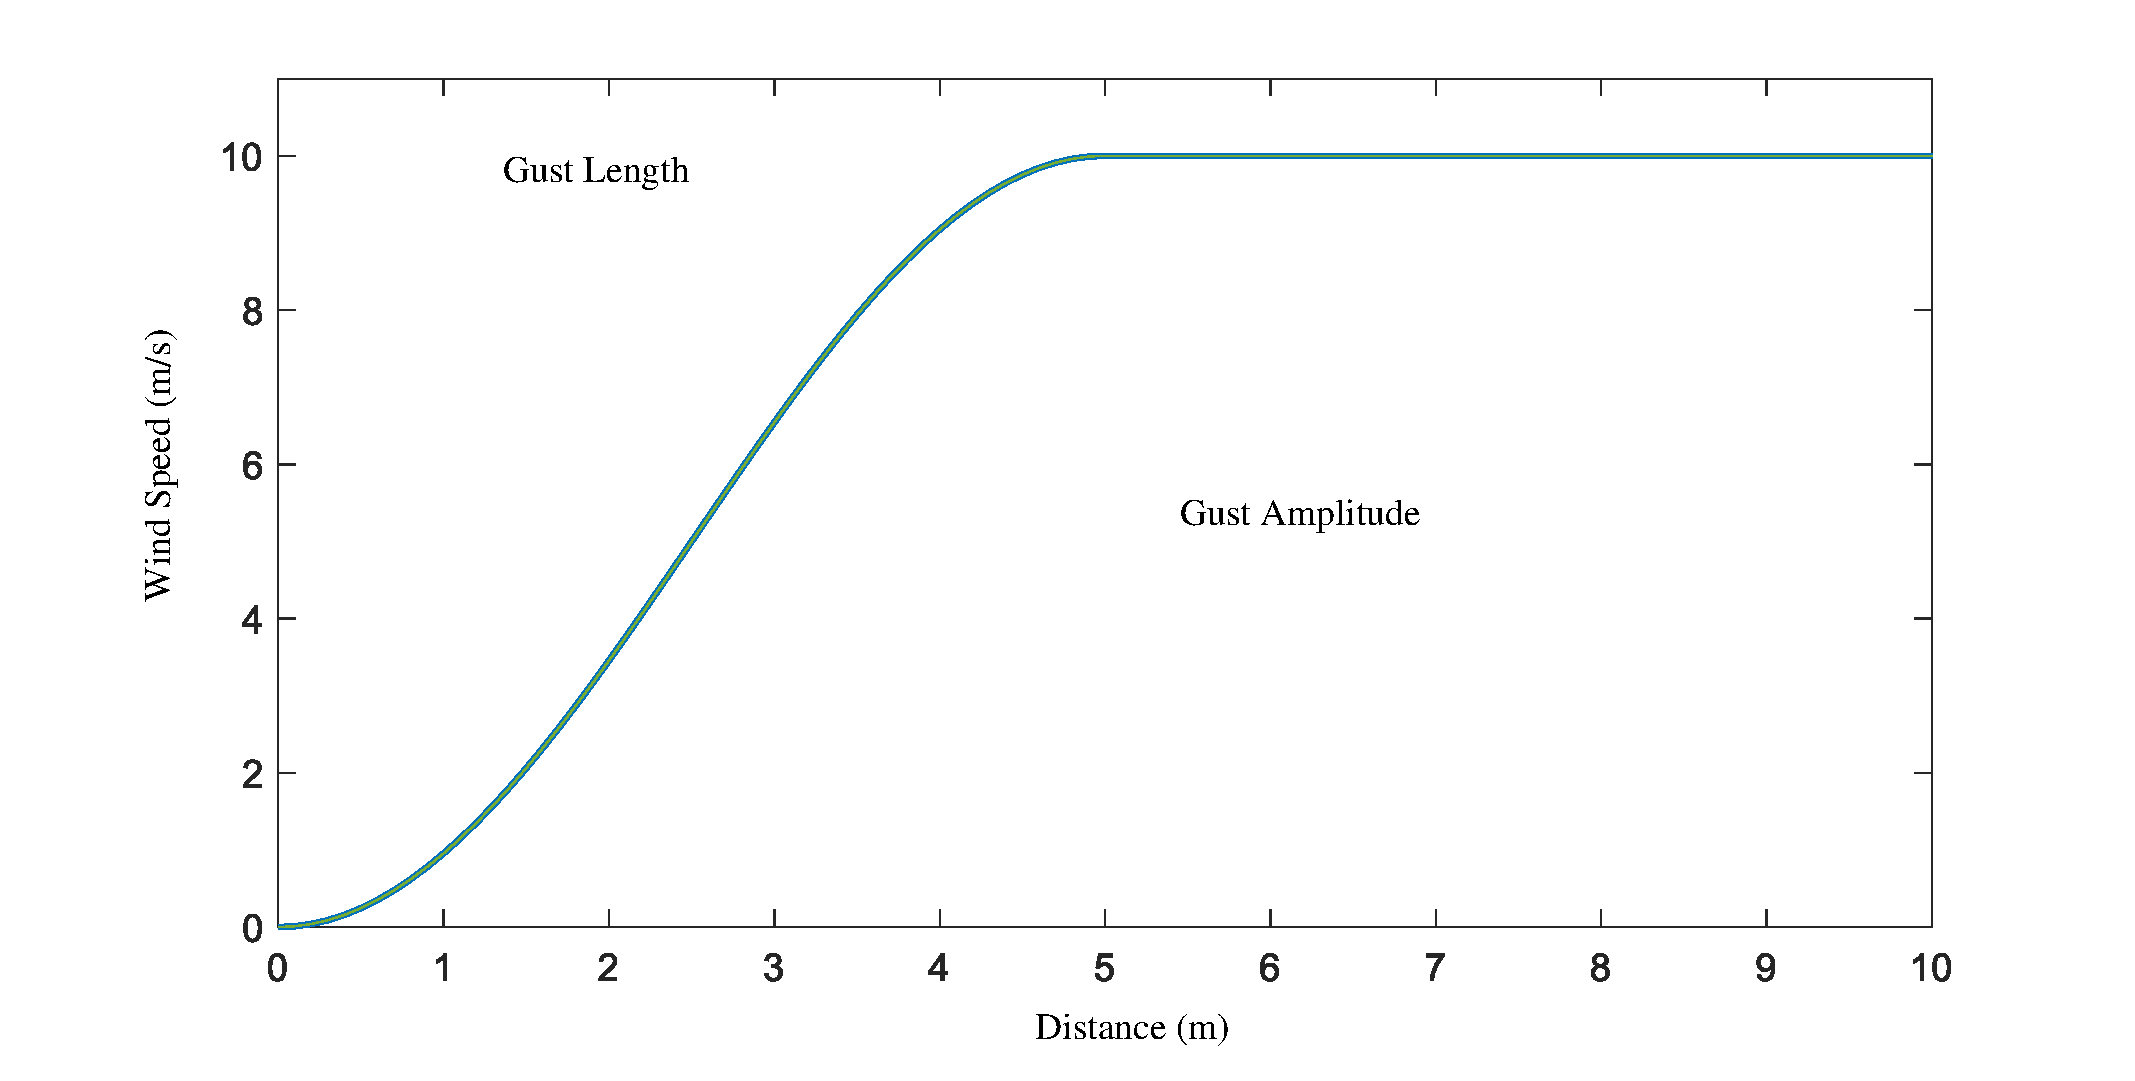
\includegraphics[width=0.8\textwidth]{Figures/Figs_Ch4/fig1.pdf}
	\caption{Half-wavelength atmospheric disturbance gust modelling\cite{ly1980time}}\label{fig1}
\end{figure}\\
the gust contains three velocity components $u_{\mathrm{G}}^{\mathrm{b}}$, $v_{\mathrm{G}}^{\mathrm{b}}$ and $w_{\mathrm{G}}^{\mathrm{b}}$ in the body coordinate system and the three velocities are uncorrelated and have the same mathematical model. The 1-cosine discrete gust model is available in both full-wavelength and half-wavelength model. Taking the velocity $u_{\mathrm{G}}^{\mathrm{b}}$ in the direction of the body axis $o_{\mathrm{b}}x_{\mathrm{b}}$ as an example, the full-wavelength 1-cosine discrete gust model is

\begin{equation}\label{eq6}
u_{\mathrm{G}}^{\mathrm{b}}(x)= \begin{cases}0 & x<0 \\ \frac{V_m}{2}\left(1-\cos \left(\frac{\pi x}{d_m}\right)\right) & 0<x<2 d_m \\ 0 & x>2 d_m\end{cases}
\end{equation}
and the half-wavelength 1-cosine discrete gust model is
\begin{equation}
u_{\mathrm{G}}^{\mathrm{b}}(x)= \begin{cases}0 & x<0 \\ \frac{V_m}{2}\left(1-\cos \left(\frac{\pi x}{d_m}\right)\right) & 0<x<d_m \\ V_m & x>d_m\end{cases}
\end{equation}
where $V_m$ denotes the gust intensity, namely, the maximum value of gust wind speed; $d_m$ denotes the gust scale, namely, the transition distance of gust establishment; $x$ denotes the distance into the gust. By applying the gust model to the three body axes of the aircraft, $u_{\mathrm{G}}^{\mathrm{b}}(x)$, $v_{\mathrm{G}}^{\mathrm{b}}(x)$ and $w_{\mathrm{G}}^{\mathrm{b}}(x)$ can be obtained.

Before the 1980s, the full-wavelength 1-cosine discrete gust model was more often used. With the continuous improvement of numerical simulation technology, the traditional full-wavelength model can no longer satisfy the needs of the study. After the 1980s, the half-wavelength 1-cosine discrete gust model is more often used. Compared with the full-wavelength 1-cosine discrete gust model, the half-wavelength 1-cosine discrete gust model is more convenient and flexible. The half-wavelength 1-cosine discrete gust model is used in the U.S. military specification MIL-F-8785C\cite{military1980u} and has been modularised in Simulink's Aerospace toolbox.

\section{Wind Shear}
Wind shear refers to the sudden change of wind direction or wind speed between any two points in space within a certain period of time, including the sudden vertical shear of horizontal winds, the horizontal shear of horizontal winds and the shear of vertical winds. Research results show that wind shear often occurs in the low and medium-altitude areas where aircraft take off and land, posing a great danger and threat to the safe operation of aircraft.

At present, there are three main ways of modeling wind shear. The first way is to store the Doppler radar measurement data in the form of a grid in the computer, and it is also possible to establish a wind shear incident database. The data is real and the amount of data storage depends on the division of the grid size, and the interpolation method can be adopted to take the values in use. However, the cost required by this method is very high; the second way is to establish and numerically solve the atmospheric dynamics equations in accordance with the laws of hydrodynamics and thermodynamics. The equations of atmospheric dynamics are nonlinearly differential and it generally takes up a lot of memory and machine time to solve to equations numerically. The real-time performance of this method is generally difficult to meet, and it is not suitable for engineering simulation; the third way is to establish an engineering simulation model, that is, to establish a relatively simplified mathematical model that describes the nature of the wind shear phenomenon, the mechanism and the movement process. This engineering wind shear model is simple and flexible, easy to use, and has better realism, so it is more suitable for atmospheric wind field simulation applications\cite{noauthor__nodate}.

The most widely used models for wind shear in the ground boundary layer are the logarithmic and exponential models. The Prandtl logarithmic model is expressed as
\begin{equation}\label{eq8}
u_{\mathrm{S}}(h)=\frac{u_{\mathrm{S} 0}}{k} \ln \frac{h}{h_0}
\end{equation}
where $h$ is the altitude; $u_{\mathrm{S0}}$ is the friction velocity, which depends on the shear stress on the ground $\tau_0$ and the air density $\rho_0$, denoted as $u_{\mathrm{S0}}=\sqrt{\tau_0/\rho_0}$; $h_0$ characterises the effect of the roughness of the ground; and $k=0.4$ is known as Karman's constant.

The exponential model for wind shear in the ground boundary layer takes the form
\begin{equation}\label{eq9}
u_{\mathrm{S}}(h)=u_{\mathrm{SR}}\left(\frac{h}{h_R}\right)^m
\end{equation}
where $h$ is the altitude; $u_{\mathrm{SR}}$ is the mean wind speed at the reference altitude $h_R$; and $m$ is the wind shear index, which is affected by factors such as ground roughness $h_0$ and temperature gradient ${dT/dh}$ \cite{gipe1993wind}.

In the U.S. Army military specification MIL-F-8785C\cite{military1980u}, the logarithmic model used for horizontal wind variation with height is
\begin{equation}\label{eq10}
u_{\mathrm{S}}(h)=W_{20} \frac{\ln \left(\frac{h}{z_0}\right)}{\ln \left(\frac{20}{z_0}\right)}, \quad 3 f t<h<1000 {ft}
\end{equation}
where $h$ is the altitude; $W_{20}$ denotes the wind speed at 20 ft above sea level; and $z_0$ takes the value of 0.15 ft for the Class $\mathbf{C}$ phase of flight (specifically defined in the literature \cite{military1980u}, which generally refers to the take-off and landing phases), and $z_{0}$ takes the value of 2.0 ft for the other phases.

It is worth noting that the wind shear velocity derived from the above model is the horizontal mean wind velocity, which can be projected in the ground coordinate system if the angle between the wind direction and the earth's axis is known. In particular, assuming that the angle between the direction of the wind and the earth's axis $o_{\mathrm{g}}x_{\mathrm{g}}$ is $\theta_{\mathrm{S}}$, the velocity component of the wind shear in the ground coordinate system is expressed as follows
\begin{equation}\label{eq11}
\mathbf{v}_{\mathrm{S}}^\mathrm{g}(h)=\left[\begin{array}{c}
u_{\mathrm{S}}^\mathrm{g}(h) \\
v_{\mathrm{S}}^\mathrm{g}(h) \\
w_{\mathrm{S}}^\mathrm{g}(h)
\end{array}\right]=\left[\begin{array}{c}
u_{\mathrm{S}}(h) \cos \theta_{\mathrm{S}} \\
u_{\mathrm{S}}(h) \sin \theta_{\mathrm{S}} \\
0
\end{array}\right]
\end{equation}
It should be noted that $h$ is the altitude, which is satisfied by $z_\mathrm{g}=-h$ in the ground coordinate system. This can then be transformed to the aircraft body coordinate system by means of the coordinate system transformation method
\begin{equation}\label{eq12}
\mathbf{v}_{\mathrm{S}}^{\mathrm{b}}(h)=\left[\begin{array}{c}
u_{\mathrm{S}}^{\mathrm{b}}(h) \\
v_{\mathrm{S}}^{\mathrm{b}}(h) \\
w_{\mathrm{S}}^{\mathrm{b}}(h)
\end{array}\right]=\mathbf{R}_{\mathrm{b} / \mathrm{g}}(\theta, \psi, \phi) \mathbf{v}_{\mathrm{S}}^{\mathrm{g}}(h)
\end{equation}
where $u_{\mathrm{S}}^{\mathrm{b}}(h)$, $v_{\mathrm{S}}^{\mathrm{b}}(h)$ and $w_{\mathrm{S}}^{\mathrm{b}}(h)$ are the three components of the induced velocity from wind shear on the aircraft body axis.

\section{Tanker Wake}
Tanker wake vortex is a kind of perturbation due to the presence of pressure differences between the upper and lower surfaces of the tanker wing, the airflow on the lower wing surface is reversed upwards around the wing tip under the effect of pressure difference to form a vortex spreading backward, thus affecting the receiver aircraft. It belongs to  non-random perturbations, related to the state of the tanker but not related to the state of the receiver. The perturbation occurs in the last four phases when the tanker and receiver aircraft are close to each other, and it can be equated to a constant angle of attack perturbation due to the small change in the relative positions of the tanker and the receiver aircraft in the docking phase.

According to the lift line theory\cite{pamadi2004performance}. Vortices from the wing and horizontal tail of a tanker can be modeled as horseshoe Vortices as shown in Fig. \ref{fig2}. Four vortex lines along the axis of the airflow coordinate system $o_{\mathrm{w}}x_{\mathrm{w}}$ are trailed by the wing tip and tail tip, which correspond to vortex line \ding{172}\ding{173}\ding{174}\ding{175} in Fig. \ref{fig2}; and two vortex lines exist in the direction of the wingspan and the tail, which correspond to vortex line \ding{176} and \ding{177} in Fig. \ref{fig2}, respectively. When the wing generates positive lift, the wing tip vortex rotates inward; when the horizontal tail generates negative lift, the tail tip vortex rotates outward. Thus, the vortices on the wing and tail are in opposite directions. Since the lift generated by the wing is much greater than that generated by the tail, the wing vortices are much stronger than the tail vortices.
\begin{figure}[th]
	\centering
	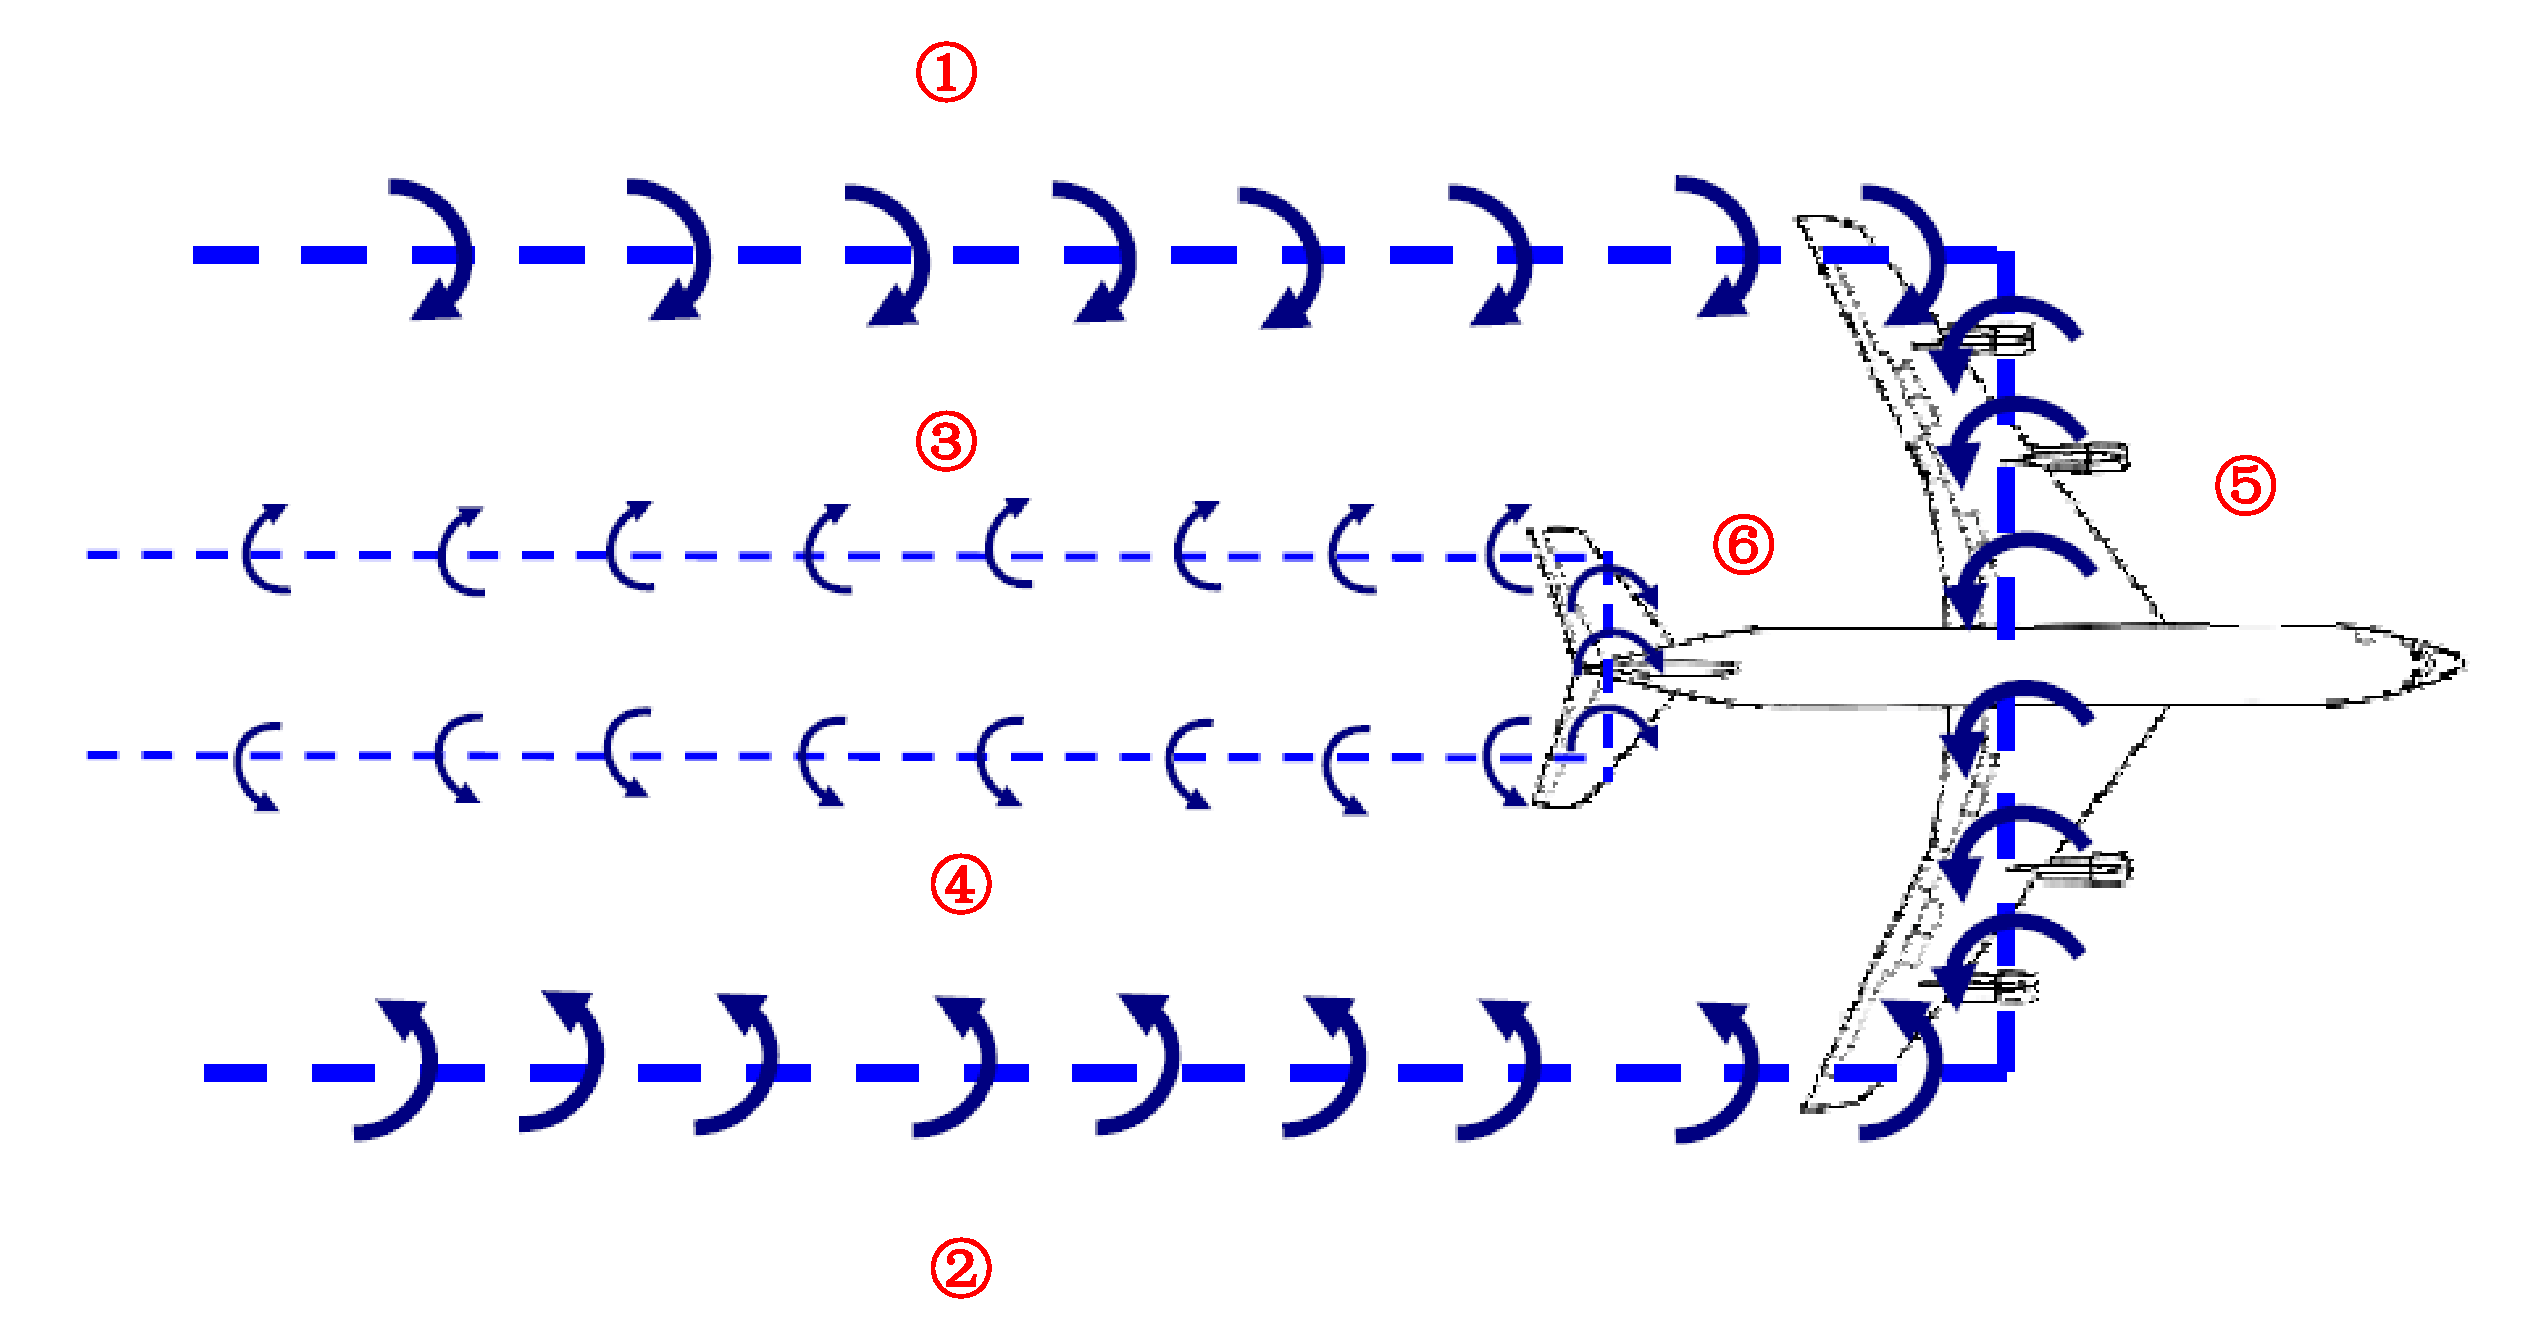
\includegraphics[width=0.9\textwidth]{Figures/Figs_Ch4/fig2.pdf}
	\caption{Schematic of the wing and horizontal tail saddle vortex\cite{pamadi2004performance}}\label{fig2}
\end{figure}

For simplicity of analysis, wingtip vortices are generally considered to be a series of circular swirling motions with the center of the circle located on the vortex line, producing induced velocities tangent to the circle. For any position in the near airspace of the tanker, it is simultaneously affected by the six vortices in Fig. \ref{fig2}. By analyzing the effect of each vortex separately and then superimposing them the total effect of the tanker wake on any position in the space can be obtained. As shown in Fig. \ref{fig3}, assuming that in the airflow coordinate system, the relative position coordinate of any point $\text{p}$ in space relative to the center of the wingtip vortex $\text{o}$ is $\mathbf{p}_{{\mathrm{p} \mathrm{\left/{\vphantom {p o}} \right.\kern-\nulldelimiterspace}\mathrm {o}}}^{\mathrm{w}} = {\left[ {\begin{array}{*{20}{c}}{x_{{\mathrm{p} \mathrm{\left/{\vphantom {p o}} \right.\kern-\nulldelimiterspace}\mathrm{o}}}^{\mathrm{w}}}&{y_{{\mathrm{p} \mathrm{\left/{\vphantom {p o}} \right.\kern-\nulldelimiterspace} \mathrm{o}}}^{\mathrm{w}}}&{z_{{\mathrm{p} \mathrm{\left/{\vphantom {p o}} \right.\kern-\nulldelimiterspace}\mathrm{o}}}^{\mathrm{w}}}\end{array}} \right]^\mathrm{T}}$; $r_{R} = \left\| {\mathbf{p}_{{\mathrm{p} \mathrm{\left/{\vphantom {p o}} \right.\kern-\nulldelimiterspace} \mathrm{o}}}^{\mathrm{w}}} \right\|$ is the radial distance from the position $\mathbf{p}$ to the vortex line; the induced velocity of the left wingtip vortex at the point $\mathbf{p}$ is $\mathbf{v}_{\mathrm{LWI}}^\mathrm{w}$, and the direction is tangent to the circular vortex; and the angle of induced velocity $\mathbf{v}_{\mathrm{LWI}}^\mathrm{w}$ and the axis of $o_{\mathrm{w}}y_{\mathrm{w}}$ in the airflow coordinate system is ${\theta _\mathrm{LWI}}$.
\begin{figure}[th]
	\centering
	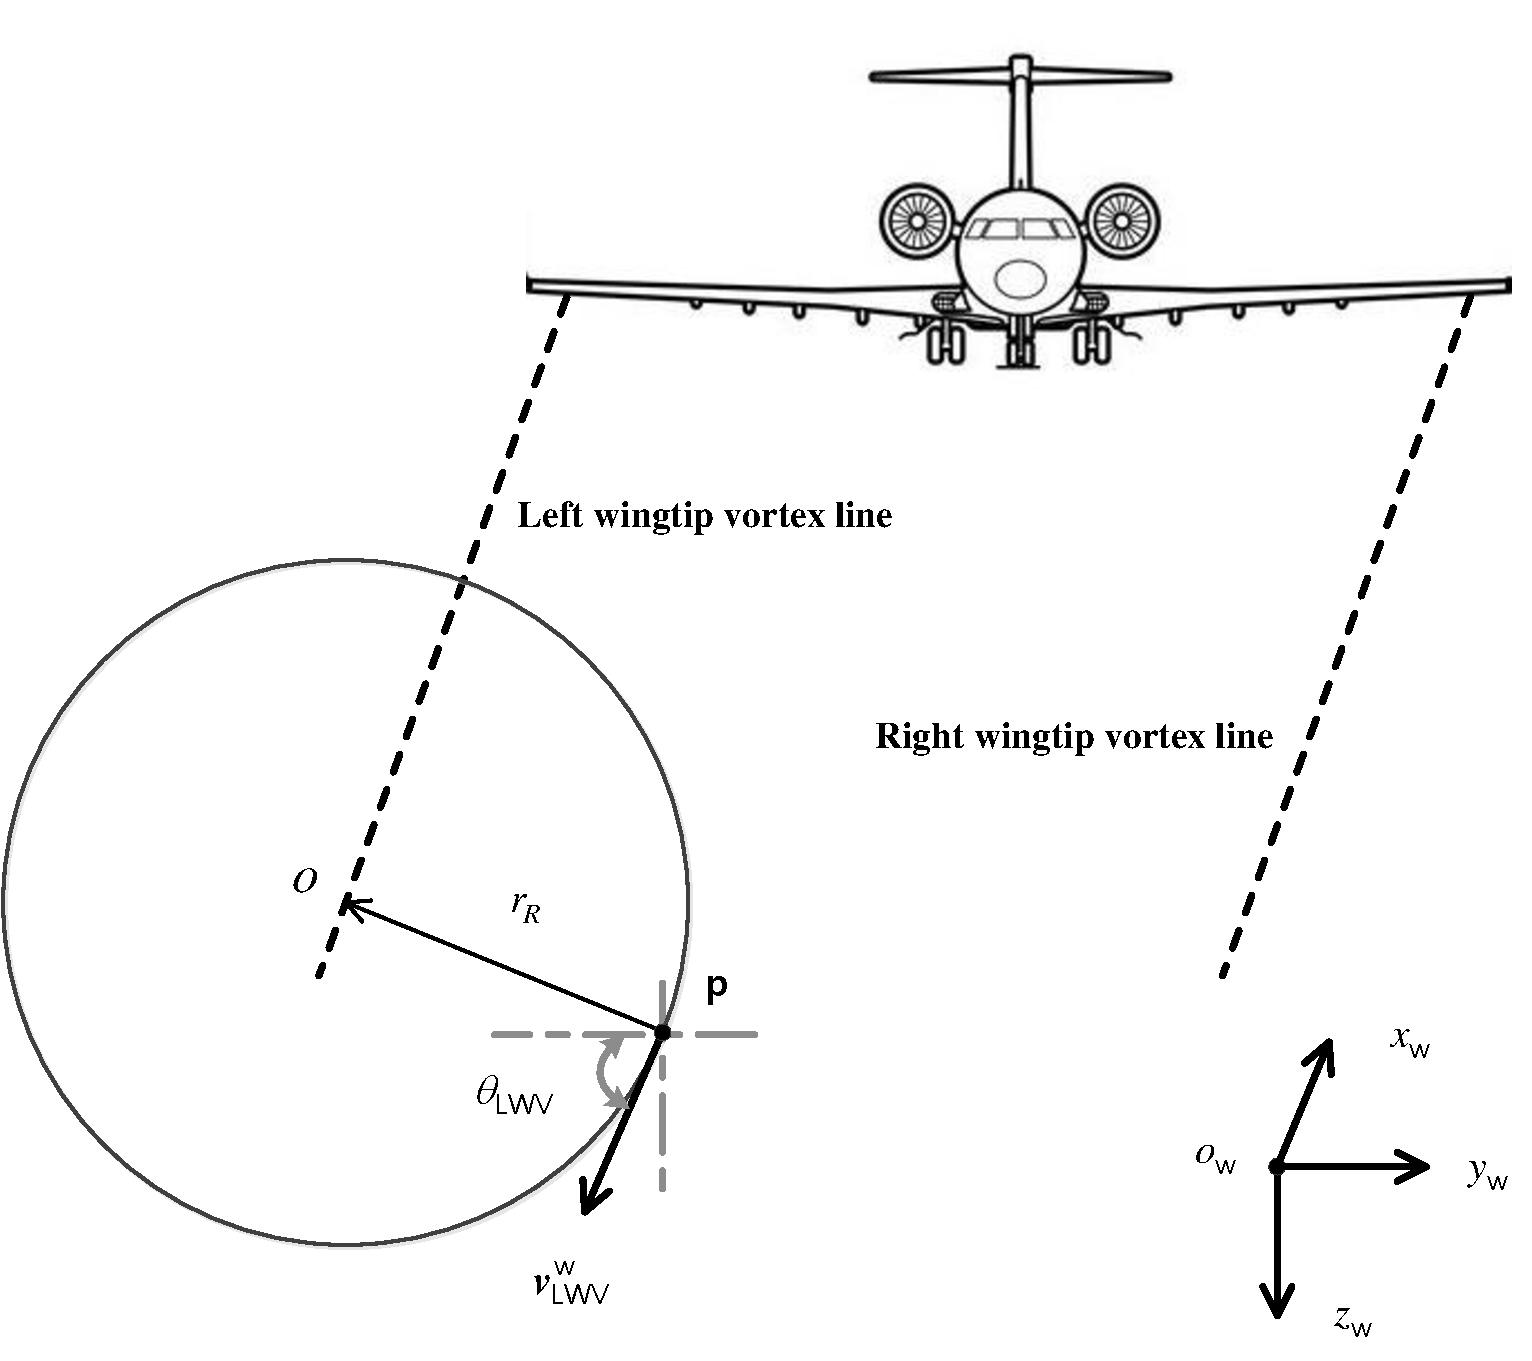
\includegraphics[width=0.6\textwidth]{Figures/Figs_Ch4/fig3.pdf}
	\caption{Schematic diagram of a tanker wake}\label{fig3}
\end{figure}

According to literature\cite{dogan2008flight}, the size of the induced velocity produced by each vortex line at the point $\mathbf{p}$ is
\begin{equation}\label{eq13}
V=\frac{\Gamma r_R}{2 \pi\left(r_R^2+r_c^2\right)}\left(1-\exp \left(-\frac{r_R^2}{4 v \tau}\right)\right)
\end{equation}
where $\Gamma$ is the vortex strength, $r_c$ is the radius of the vortex core which can be taken as $r_c=2.24\sqrt{\upsilon\tau}$, $\upsilon$ is the viscosity coefficient which can be taken as $\upsilon=0.06\times\Gamma$, $\tau$ is the vortex time coefficient related to the airspeed of the tanker,  $r_{R} = \left\| {\mathbf{p}_{{\mathrm{p} \mathrm{\left/{\vphantom {p o}} \right.\kern-\nulldelimiterspace} \mathrm{o}}}^{\mathrm{w}}} \right\|$ is the radial distance from the position $\mathbf{p}$ to the vortex line.

The vortex strength can be calculated by the following equation as follows 
\begin{equation}\label{eq14}
\Gamma=\frac{L}{\rho V_t(\pi / 4) b} \frac{\cos \gamma_1+\cos \gamma_2}{2}
\end{equation}
where $b$ is the wingspan of the tanker, $\rho$ is the air density, $V_t$ is the airspeed of the tanker, and $L$ is the lift generated by the wings or tail of the tanker; $\gamma_1$ and $\gamma_2$ is the angle from the end point of the vortex line to the current point. For bound vortices, namely, vortex lines \ding{176}\ding{177} in Fig. \ref{fig2}, both $\gamma_1$ and $\gamma_2$ are non-zero; for tip vortices, namely, vortex lines \ding{172}\ding{173}\ding{174}\ding{175} in Fig. \ref{fig2}, $\gamma_1$ and $\gamma_2$ are equal to zero.

According to Eqs. (\ref{eq13}) and (\ref{eq14}), the induced velocities of the six vortices generated at any point $\mathbf{p}$ in the space can be calculated, including left wingtip vortex $\mathbf{v}^\mathrm{w}_\mathrm{LWV}$, right wingtip vortex $\mathbf{v}^\mathrm{w}_\mathrm{RWV}$, left tailtip vortex $\mathbf{v}^\mathrm{w}_\mathrm{LTV}$, right tailtip vortex $\mathbf{v}^\mathrm{w}_\mathrm{RTV}$, wing spreading vortex $\mathbf{v}^\mathrm{w}_\mathrm{WV}$ and horizontal tail spreading vortex $\mathbf{v}^\mathrm{w}_\mathrm{TV}$, respectively. The components of $\mathbf{v}^\mathrm{w}_\mathrm{LWV}$, $\mathbf{v}^\mathrm{w}_\mathrm{RWV}$, $\mathbf{v}^\mathrm{w}_\mathrm{LTV}$ and $\mathbf{v}^\mathrm{w}_\mathrm{RTV}$ lie in the plane of the airflow coordinate system ${o}_\mathrm{w}{y}_\mathrm{w}{z}_\mathrm{w}$ and therefore have a component of 0 along the $o_\mathrm{w}x_\mathrm{w}$ axis, while $\mathbf{v}_\mathrm{WI}^\mathrm{w}$ and $\mathbf{v}_\mathrm{TV}^\mathrm{w}$ lie in the plane of the airflow coordinate system ${o}_\mathrm{w}{x}_\mathrm{w}{z}_\mathrm{w}$ and therefore have a component of 0 along the ${o}_\mathrm{w}{y}_\mathrm{w}$ axis. Taking the induced velocity $\mathbf{v}^\mathrm{w}_\mathrm{LWV}$ generated by the left wingtip vortex in Fig. \ref{fig3} as an example, its component in the airflow coordinate system can be expressed as
\begin{equation}\label{eq15}
\mathbf{v}_{\mathrm{LWV}}^{\mathrm{w}}=\left[\begin{array}{c}
0 \\
-V_{\mathrm{LWV}} \cos \theta_{\mathrm{LWV}} \\
V_{\mathrm{LWV}} \sin \theta_{\mathrm{LWV}}
\end{array}\right]
\end{equation}
where $V_\mathrm{LWV}$ is the magnitude of the induced velocity generated by the left wingtip vortex, which can be calculated according to Eq. (\ref{eq13}). All other induced velocities can be decomposed into the airflow coordinate system. Specifically, in the aerial refueling process, the point $\mathbf{p}$ is the position of the receiver aircraft, and the direction of induced speed can be determined according to the relative position relationship between the receiver and the tanker.

The total induced velocity $\mathbf{v}^\mathrm{w}_\mathrm{V}$ generated by the tanker wake at any point in space can be obtained by summing the induced velocity generated by the six eddies at that point, which is expressed as follows
\begin{equation}\label{eq16}
\mathbf{v}_{\mathrm{V}}^{\mathrm{w}}(x, y, z)=\mathbf{v}_{\mathrm{LWV}}^{\mathrm{w}}+\mathbf{v}_{\mathrm{RWV}}^{\mathrm{w}}+\mathbf{v}_{\mathrm{LTV}}^{\mathrm{w}}+\mathbf{v}_{\mathrm{RTV}}^{\mathrm{w}}+\mathbf{v}_{\mathrm{WV}}^{\mathrm{w}}+\mathbf{v}_{\mathrm{TV}}^{\mathrm{w}}
\end{equation}
from the analysis, it can be seen that the induced speed generated by the tanker wake is a function of position. The total induced velocity $\mathbf{v}^\mathrm{w}_\mathrm{V}$ is decomposed into three components along the axial direction in the airflow coordinate system
\begin{equation}\label{eq17}
\mathbf{v}_{\mathrm{V}}^{\mathrm{w}}(x, y, z)=\left[\begin{array}{lll}
u_{\mathrm{V}}^{\mathrm{w}} & v_{\mathrm{V}}^{\mathrm{w}} & w_{\mathrm{V}}^{\mathrm{w}}
\end{array}\right]^{\mathrm{T}}
\end{equation}
According to the coordinate system conversion method introduced in chapter 2, the total induced velocity $\mathbf{v}^\mathrm{w}_\mathrm{V}$ in the airflow coordinate system can be transformed into the receiver aircraft body coordinate system. In the receiver aircraft body coordinate system, Eq. (\ref{eq16}) can be rewritten as 
\begin{equation}\label{eq18}
\mathbf{v}_{\mathrm{V}}^{\mathrm{r}}(x, y, z)=\mathbf{R}_{\mathrm{r} / \mathrm{w}}(\alpha, \beta) \mathbf{v}_{\mathrm{V}}^{\mathrm{w}}(x, y, z)=\left[\begin{array}{lll}
u_{\mathrm{V}}^{\mathrm{r}} & v_{\mathrm{V}}^{\mathrm{r}} & w_{\mathrm{V}}^{\mathrm{r}}
\end{array}\right]^{\mathrm{T}}
\end{equation}
where $\mathbf{R}_\mathrm{r / w}(\alpha, \beta)$=$\mathbf{R}_\mathrm{b / w}(\alpha,\beta)$, $\alpha$ and $\beta$ are the angle of attack and side slip angle of the receiver, respectively, and the velocity components $u^\mathrm{r}_\mathrm{V}$, $v^\mathrm{r}_\mathrm{V}$ and $w^\mathrm{r}_\mathrm{V}$ are all functions of position.

Based on the literature\cite{pamadi2004performance}, the non-uniform wind field can be approximately decomposed into a uniform wind disturbance component and a uniform wind gradient component, namely, translational wind speed and rotating wind speed. Therefore, the induced angular velocity $\boldsymbol{\omega}_\mathrm{V}^\mathrm{r}\left( {x,y,z} \right) = {\left[ {\begin{array}{*{20}{c}}
		{p_\mathrm{V}^\mathrm{r}}&{q_\mathrm{V}^\mathrm{r}}&{r_\mathrm{V}^\mathrm{r}}
		\end{array}} \right]^\mathrm{T}}$ generated by the tanker wake can be obtained as
\begin{equation}\label{eq19}
\begin{aligned}
& p_{\mathrm{V}}^{\mathrm{r}}=\frac{\partial w_{\mathrm{V}}^{\mathrm{r}}}{\partial y}-\frac{\partial v_{\mathrm{V}}^{\mathrm{r}}}{\partial z} \\
& q_{\mathrm{V}}^{\mathrm{r}}=\frac{\partial u_{\mathrm{V}}^{\mathrm{r}}}{\partial z}-\frac{\partial w_{\mathrm{V}}^{\mathrm{r}}}{\partial x} \\
& r_{\mathrm{V}}^{\mathrm{r}}=\frac{\partial v_{\mathrm{V}}^{\mathrm{r}}}{\partial x}-\frac{\partial u_{\mathrm{V}}^{\mathrm{r}}}{\partial y}
\end{aligned}
\end{equation}
where $p^\mathrm{r}_\mathrm{V}$, $q^\mathrm{r}_\mathrm{V}$ and $r^\mathrm{r}_\mathrm{V}$ are the components of the induced angular velocity generated by the tanker wake stream on the receiver aircraft body axis, respectively.
\section{Bow Wave Effect}
In the probe-and-drogue aerial refueling docking process, when the drogue and the receiver aircraft are very close to each other, the airflow near the nose of the receiver aircraft produces a strong aerodynamic disturbance to the drogue, pushing the drogue away from the probe, This phenomenon is called as the bow wave effect. It should be noted that the modeling of the bow wave is different from the modeling of the bow wave effect.The bow wave effect is essentially due to that the airflow changes after passing over the nose of the aircraft. The drogue swings in the changed flow field, and experiences a force similar to the repulsive force generated by the aircraft's nose. The term ``bow wave'' refers to the airflow that has passed over the aircraft's nose. Modeling the bow wave involves modeling the flow field of this airflow, which
is unrelated to the drogue. On the other hand, the term ``bow wave effect'' pertains to the changes experienced by the drogue due to the bow wave. Essentially, modeling the bow wave effect involves capturing the disturbances affecting the drogue, such as modeling the forces acting on the drogue in the presence of the bow wave.

From the perspective of flow field theory, this section will first model the bow wave, namely, the flow field near the nose, and then analyze the force of the drogue in the flow field. According to the classical fluid dynamics theory, the flow of uniform velocity air over some simple objects, such as cylinders and symmetric wings, can be modeled by the method of stream function. However, the stream function approach is only applicable to non-viscous fluids. If the viscosity of air want to be considered, additional calibration functions need to be incorporated. To reduce the model complexity, this section first introduces the modeling method of the two-dimensional flow field of the nose profile, which is then mapped to the three-dimensional spatial flow field distribution. After obtaining the flow field distribution, a similar method of aircraft wind disturbance modeling can be used to obtain the magnitude and direction of the force subjected to the drogue, which can then be substituted into the dynamic equation of the hose-drogue system to better simulate the dynamic motion of the drogue under the receiver aircraft bow wave disturbance.
\subsection{Stream functions}
By varying the distribution and intensity of the basic flow field unit (source, sink, doublet), some complex flow fields bypassing something can be described, for example, the induced flow field when the airflow flows through the aircraft nose. Line doublet are well suited for modeling the three-dimensional flow field around the nose and fuselage, but they are not effective for modeling the flow field of a pressurized body (e.g. a wing). As shown in Fig. \ref{fig4}, considering the longitudinal section of the nose, a two-dimensional stream function coordinate system $oxy$ is established by taking the apex of the nose as the origin. Considering that the bow wave effect only arises when the distance between the receiver and the drogue is very close, and the bow wave effect decreases sharply with the increase of the distance between the receiver and the drogue. Meanwhile, the drogue only moves in a limited area during the docking stage. Therefore, the modeling region is set as the dashed box region in Fig. \ref{fig4}. According to the literature \cite{rauscher1953introduction}, assuming that the linear doublet intensity distribution function distributed on the $[x_a,x_b]$ 
interval of the $x$-axis satisfies $f_m(x)$, the stream function $\psi{(x,y)}$ corresponding to this pair of doublet can be expressed as
\begin{equation}\label{eq20}
\psi(x, y)=V_{\infty} y-V_{\infty} y \int_{x_a}^{x_b} \frac{f_m(s)}{(x-s)^2+y^2} \mathrm{~d} s
\end{equation}
where $V_\infty$ is the free stream velocity, which is equal in magnitude and opposite in direction to the receiver airspeed, and $f_m(s)$ depends only on the shape of the nose. In practice, $x_a$ and $x_b$ should be selected first, and then ${f}_m(s)$ should be obtained by solving the boundary conditions. In general, $x_a\geq0$ and $x_b\geq1.5l$, where $l$ is the length of the nose in the modeled region.

The conditions that need to be satisfied for the doublet-constructed stream function to coincide with the actual nose flow field are called boundary conditions. A boundary condition is a constraint on a streamline that defines a boundary that no streamline can cross. By solving $\psi(x,y)=0$, a closed curve in the plane can be obtained, which corresponds to the innermost streamline in Fig. \ref{fig4} and is called ``0 streamline''. When the 0-flowline, $\psi(x,y)=0$, coincides with the nose contour line, $OA$, all the outer flowlines, $\psi>0$, flow along the 0-flowline layer but not through it. Therefore, this stream function can be used for an equivalent flow around the curve $\psi(x,y)=0$ (nose contour) when the boundary conditions are met.
\begin{figure}[th]
	\centering
	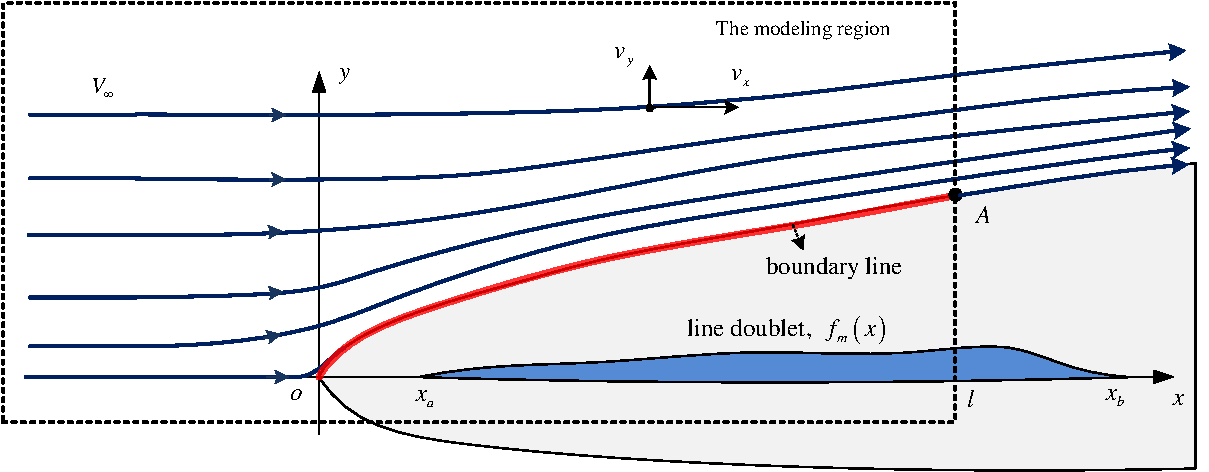
\includegraphics[width=0.8\textwidth]{Figures/Figs_Ch4/fig4.pdf}
	\caption{Airflow in the nose described by doublet stream function}\label{fig4}
\end{figure}

In Fig. \ref{fig4}, the contour line $OA$ on the upper side of the nose is selected as the boundary line, then the boundary condition can be expressed as
\begin{equation}\label{eq21}
\forall\left(x_{c_i}, y_{c_i}\right) \in O A \quad \Rightarrow \quad \psi\left(x_{c_i}, y_{c_i}\right)=0
\end{equation}
Eq. (\ref{eq21}) shows that $\psi(x,y)=0$ is satisfied at any point on the boundary line $OA$. Combining Eq. (\ref{eq20}) with the assumption of $y_{c_i}\neq0$, the boundary condition reduces to
\begin{equation}\label{eq22}
\forall\left(x_{c_i}, y_{c_i}\right) \in O A \quad \Rightarrow \quad \int_{x_a}^{x_b} \frac{f_m(s)}{\left(x_{c_i}-s\right)^2+y_{c_i}^2} \mathrm{~d} s=1
\end{equation}
$f_m(s)$ can be obtained by solving Eq. (\ref{eq22}), and then the stream function $\psi(x,y)$ can be determined from Eq. (\ref{eq20}).

A numerical calculation method to calculate the linear doublet intensity distribution function $f_m(x)$ is introduced below. As shown in Fig. \ref{fig5}, the $n$ points $\mathbf{p}_i(i=1,2,\ldots,n)$ are selected on the upper side contour line $OA$ of the nose, and the corresponding coordinates are $(x_{c_i},y_{c_i})(i=1,2,\ldots,n)$, respectively, while the linear doublet is divided into equal-length $m(m<n)$ segments on the interval $\left[ {{x_a},{x_b}} \right]$. Thus, the numerical form of Eq. (\ref{eq22}) can be expressed numerically as
\begin{equation}\label{eq23}
\sum_{j=1}^m \frac{f_m\left(s_j\right) \Delta s}{\left(x_{c_i}-s_j\right)^2+y_{c_i}^2}=1, i=1, \cdots, n
\end{equation}
where
\begin{equation}\label{eq24}
\Delta s=\frac{x_b-x_a}{m}, s_j=x_a+\frac{j}{2} \Delta s .
\end{equation}
let
\begin{equation}\label{eq25}
a_{i j}=\frac{\Delta s}{\left(x_{c_i}-s_j\right)^2+y_{c_i}^2}
\end{equation}

\begin{figure}[th]
	\centering
	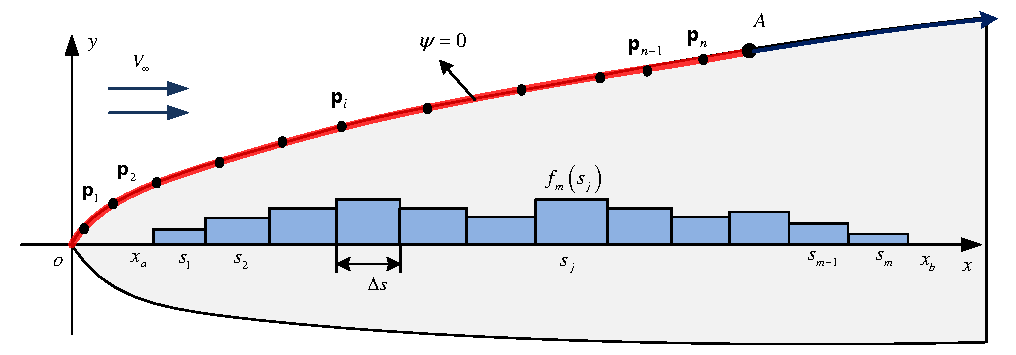
\includegraphics[width=0.8\textwidth]{Figures/Figs_Ch4/fig5.pdf}
	\caption{Numerical approach to solving boundary conditions}\label{fig5}
\end{figure} \noindent
Eq. (\ref{eq23}) can be expressed as
\begin{equation}\label{eq26}
\sum_{j=1}^m a_{i j} f_m\left(s_j\right)=1, i=1, \cdots, n
\end{equation}
or expressed as a matrix
\begin{equation}\label{eq27}
\mathbf{A}\left[\begin{array}{c}
f_m\left(s_1\right) \\
f_m\left(s_1\right) \\
\vdots \\
f_m\left(s_m\right)
\end{array}\right]=\mathbf{I}_{n \times 1}
\end{equation}
where $\mathbf{A}=(a_{ij})_{n\times m}$. Therefore, the least squares method can be used to solve Eq. (\ref{eq27}) in $f_m(s_1)$, $f_m(s_1)$, ..., $f_m(s_m)$. Thus, the numerical stream function applicable to the modeling of the flow field can be obtained
\begin{equation}\label{eq28}
\psi(x, y)=V_{\infty} y-V_{\infty} y \sum_{j=1}^m \frac{f_m\left(s_j\right) \Delta s}{\left(x-s_j\right)^2+y^2}
\end{equation}
when $m$ is large enough, the stream function obtained by the above equation has a high accuracy, but it will produce a large amount of computation, and at the same time, this method is not conducive to theoretical analysis. Thus, another analytical method for solving the stream function is introduced below.

After $f_m(s_1)$, $f_m(s_1)$,..., $f_m(s_m)$ are obtained from Eq. (\ref{eq27}), the analytical solution of $f_m(s)$ can be obtained by polynomial fitting method. For example, when the accuracy requirement is not high, a first order polynomial can be used for fitting
\begin{equation}\label{eq29}
f_m(s)=m_0+m_1 s
\end{equation}
where $m_0$ and $m_1$ are polynomial coefficients that can be obtained by fitting. Then the Eqs. (\ref{eq29}) is substituted into (\ref{eq20}), to get the analytical form of the stream function\\
\begin{equation}\label{eq30}
\begin{aligned}
\psi(x, y) & =V_{\infty} y-V_{\infty} \cdot \int_{x_a}^{x_b} \frac{\left(m_0+m_1 x\right) y}{(x-s)^2+y^2} \mathrm{~d} s \\
& =V_{\infty} y-V_{\infty}\left(m_0+m_1 x\right)\left(\tan ^{-1}\left(\frac{x_b-x}{y}\right)-\tan ^{-1}\left(\frac{x_a-x}{y}\right)\right) \\
& -0.5 m_1 V_{\infty} y\left(\ln \left(\left(\frac{x_b-x}{y}\right)^2+1\right)-\ln \left(\left(\frac{x_a-x}{y}\right)^2+1\right)\right) \, .
\end{aligned}
\end{equation}

The resulting analytical solution of the stream function is more suitable for theoretical analysis and nonlinear controller design. However, when the shape of the nose of the receiver is relatively complex, the first-order polynomial in Eq. (\ref{eq29}) is challenging to achieve the accuracy requirements, so the higher-order polynomial functions are required. As the order of the polynomial increases, the Eq. (\ref{eq30}) becomes very complex. Therefore, there is a trade-off between accuracy and complexity in practical applications.

To verify the validity of the stream function method introduced above, parameters $x_a=0.1$ and $x_2=2.5$ of the linear doublet distribution interval were taken, and $n=30$ sampling points were taken on the boundary line for simulation experiments. The experimental results are shown in Fig. \ref{fig6}. The streamlines of Fig. \ref{fig6} (a), (b) are obtained from the numerical stream function Eq. (\ref{eq28}), where the parameter values are $m=9$ and $m=20$, respectively. The streamlines in Fig. \ref{fig6} (c) is obtained from the analytic stream function Eq. (\ref{eq30}), where the parameters are $m_0=0.03$ and $m_1=0.09$.

\begin{figure}[th]
	\centering
	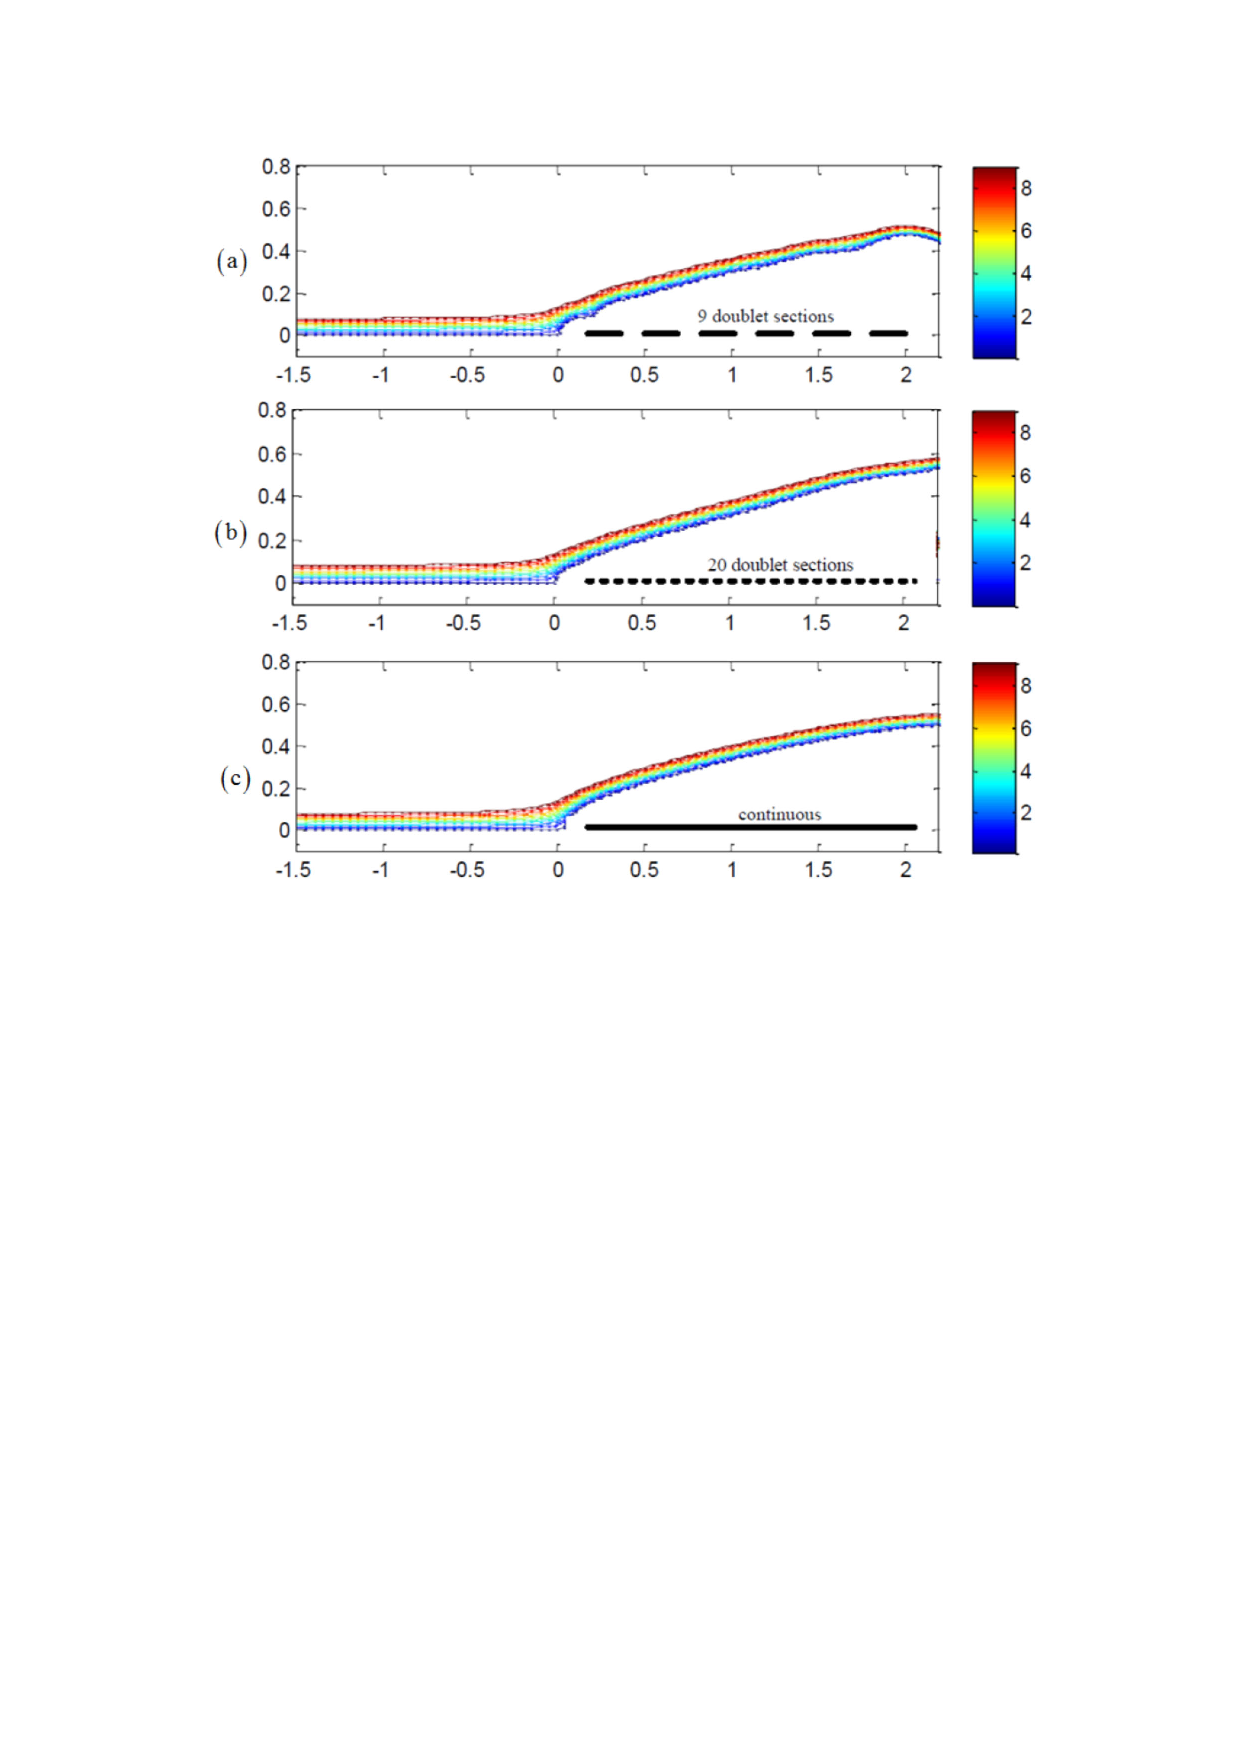
\includegraphics[width=0.6\textwidth]{Figures/Figs_Ch4/fig6.pdf}
	\caption{Streamlines generated by linear doublet with different distributions}\label{fig6}
\end{figure}

From Fig. \ref{fig6}, it can be observed that the horizontal streamlines flow along the boundary line in the presence of a linear doublet, which is in line with the desired result. Comparing Fig. \ref{fig6} (a) and Fig. \ref{fig6} (b), it can be observed that when $m$ is large enough, the numerical stream function Eq. (\ref{eq28}) produces smooth enough streamlines. At the same time, the simplified analytical stream function Eq. (\ref{eq30}) can produce streamlines that are close to those of the numerical method, but the computational effort is much smaller than that of the numerical method.

\subsection{Two-dimensional flow field and correction of the aircraft nose}
After obtaining the stream function $\psi \left( {x,y} \right)$, the distribution of the flow velocity around the aircraft nose can be obtained by the following partial differential equation\cite{rauscher1953introduction}
\begin{equation}\label{eq31}
v_x(x, y)=\frac{\partial \psi(x, y)}{\partial y}, v_y(x, y)=-\frac{\partial \psi(x, y)}{\partial x} \, .
\end{equation}

In the two-dimensional stream function coordinate system shown in Fig. \ref{fig4}, since the original velocity is $v_x=V_\infty$, $v_y=0$, the induced velocity components $u_p$ and $u_n$ due to the bow wave effect can be expressed as
\begin{equation}\label{eq32}
u_p=v_x-V_{\infty}, u_n=v_y .
\end{equation}
where $u_p$ is along the $ox$ axis and $u_n$ is along the $oy$ axis. Substituting the expression of $\psi(x,y)$, leads to
\begin{equation}\label{eq33}
\left\{\begin{array}{l}
u_p(x, y)=-V_{\infty} \int_{x_a}^{x_b} \frac{f_m(s)\left((x-s)^2-y^2\right)}{\left((x-s)^2+y^2\right)^2} \mathrm{~d} s \\
u_n(x, y)=-V_{\infty} \int_{x_a}^{x_b} \frac{2 f_m(s)(x-s) y}{\left((x-s)^2+y^2\right)^2} \mathrm{~d} s
\end{array}\right.
\end{equation}

It should be noted that the classical stream function method is proposed under the assumption that the air is an ideal steady flow with no viscosity, but in fact, the viscosity of the air and the friction of the nose surface will accelerate the attenuation of the flow field. After many CFD simulations and verifications, a correction function is introduced to compensate for air viscosity, friction, turbulence and other factors, and its expression can be expressed as
\begin{equation}\label{eq34}
\left[\begin{array}{c}
\bar{u}_p(x, y) \\
\bar{u}_n(x, y)
\end{array}\right]=\left[\begin{array}{l}
u_p(x, y) e^{-k_{u_p} r_u(x, y)} \\
u_n(x, y) e^{-k_{u_n} r_u(x, y)}
\end{array}\right]
\end{equation}
where $k_u\approx 1$ is the attenuation coefficient and $r_u(x,y)$ is a distance function that describes the distance from the point$(x,y)$ to the surface of the nose, which can be approximated by the stream function $\psi(x,y)$ 
\begin{equation}\label{eq35}
r_u(x, y)= \begin{cases}\frac{|\psi(x, y)|}{V_{\infty}} & , x \geq 0\quad m \\ \frac{\sqrt{\psi(x, y)^2+\left(V_{\infty} y\right)^2}}{V_{\infty}} & , x<0\quad m\end{cases}
\end{equation}

Fig. \ref{fig7} depicts the isogram of $r_u(x,y)$ in the above equation. The result shows that Eq. (\ref{eq35}) can measure the distance from any point to the boundary line very well. More importantly, the distance function can make full use of the calculated result $\psi(x,y)$ of Eq. (\ref{eq20}), which makes the calculation easier.\clearpage
\begin{figure}[th]
	\centering
	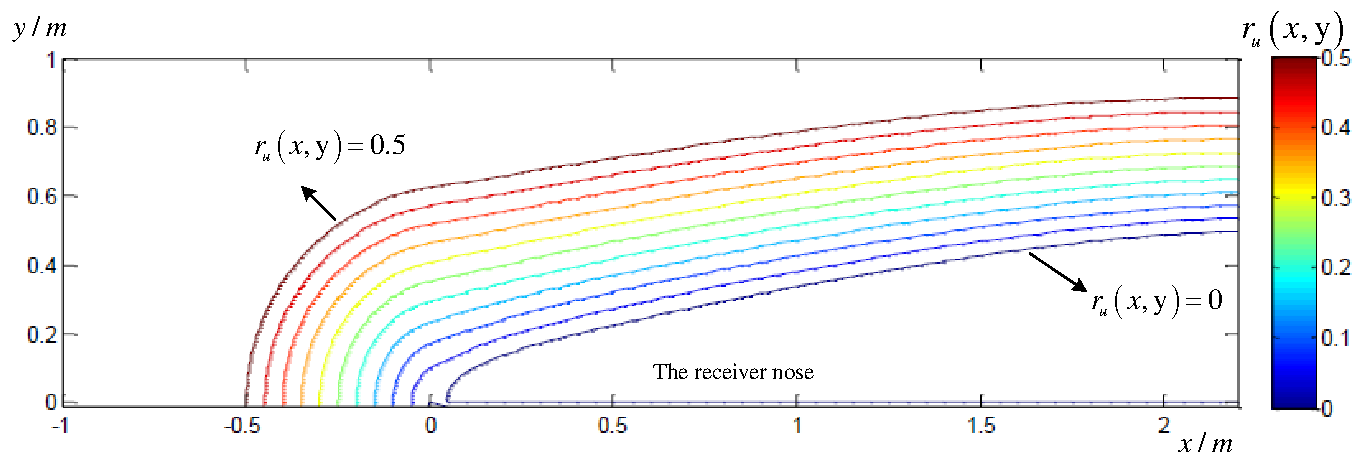
\includegraphics[width=0.8\textwidth]{Figures/Figs_Ch4/fig7.pdf}
	\caption{Isogram of the distance function $r_u(x,y)$ in the range $0<r_u<0.5m$}\label{fig7}
\end{figure}

The comparison between the final obtained velocity field distribution in the nose and the CFD experimental results is shown in Fig. \ref{fig8}, where the left figures show the results of the CFD test, and the top figure and bottom figure correspond to the velocity distributions in the directions of the $x$ and $y$ axes, respectively, and the right figures are the results obtained by the proposed method in the paper. The comparison results verify that the proposed scheme can simulate the nose-induced flow field better.
\begin{figure}[th]
	\centering
	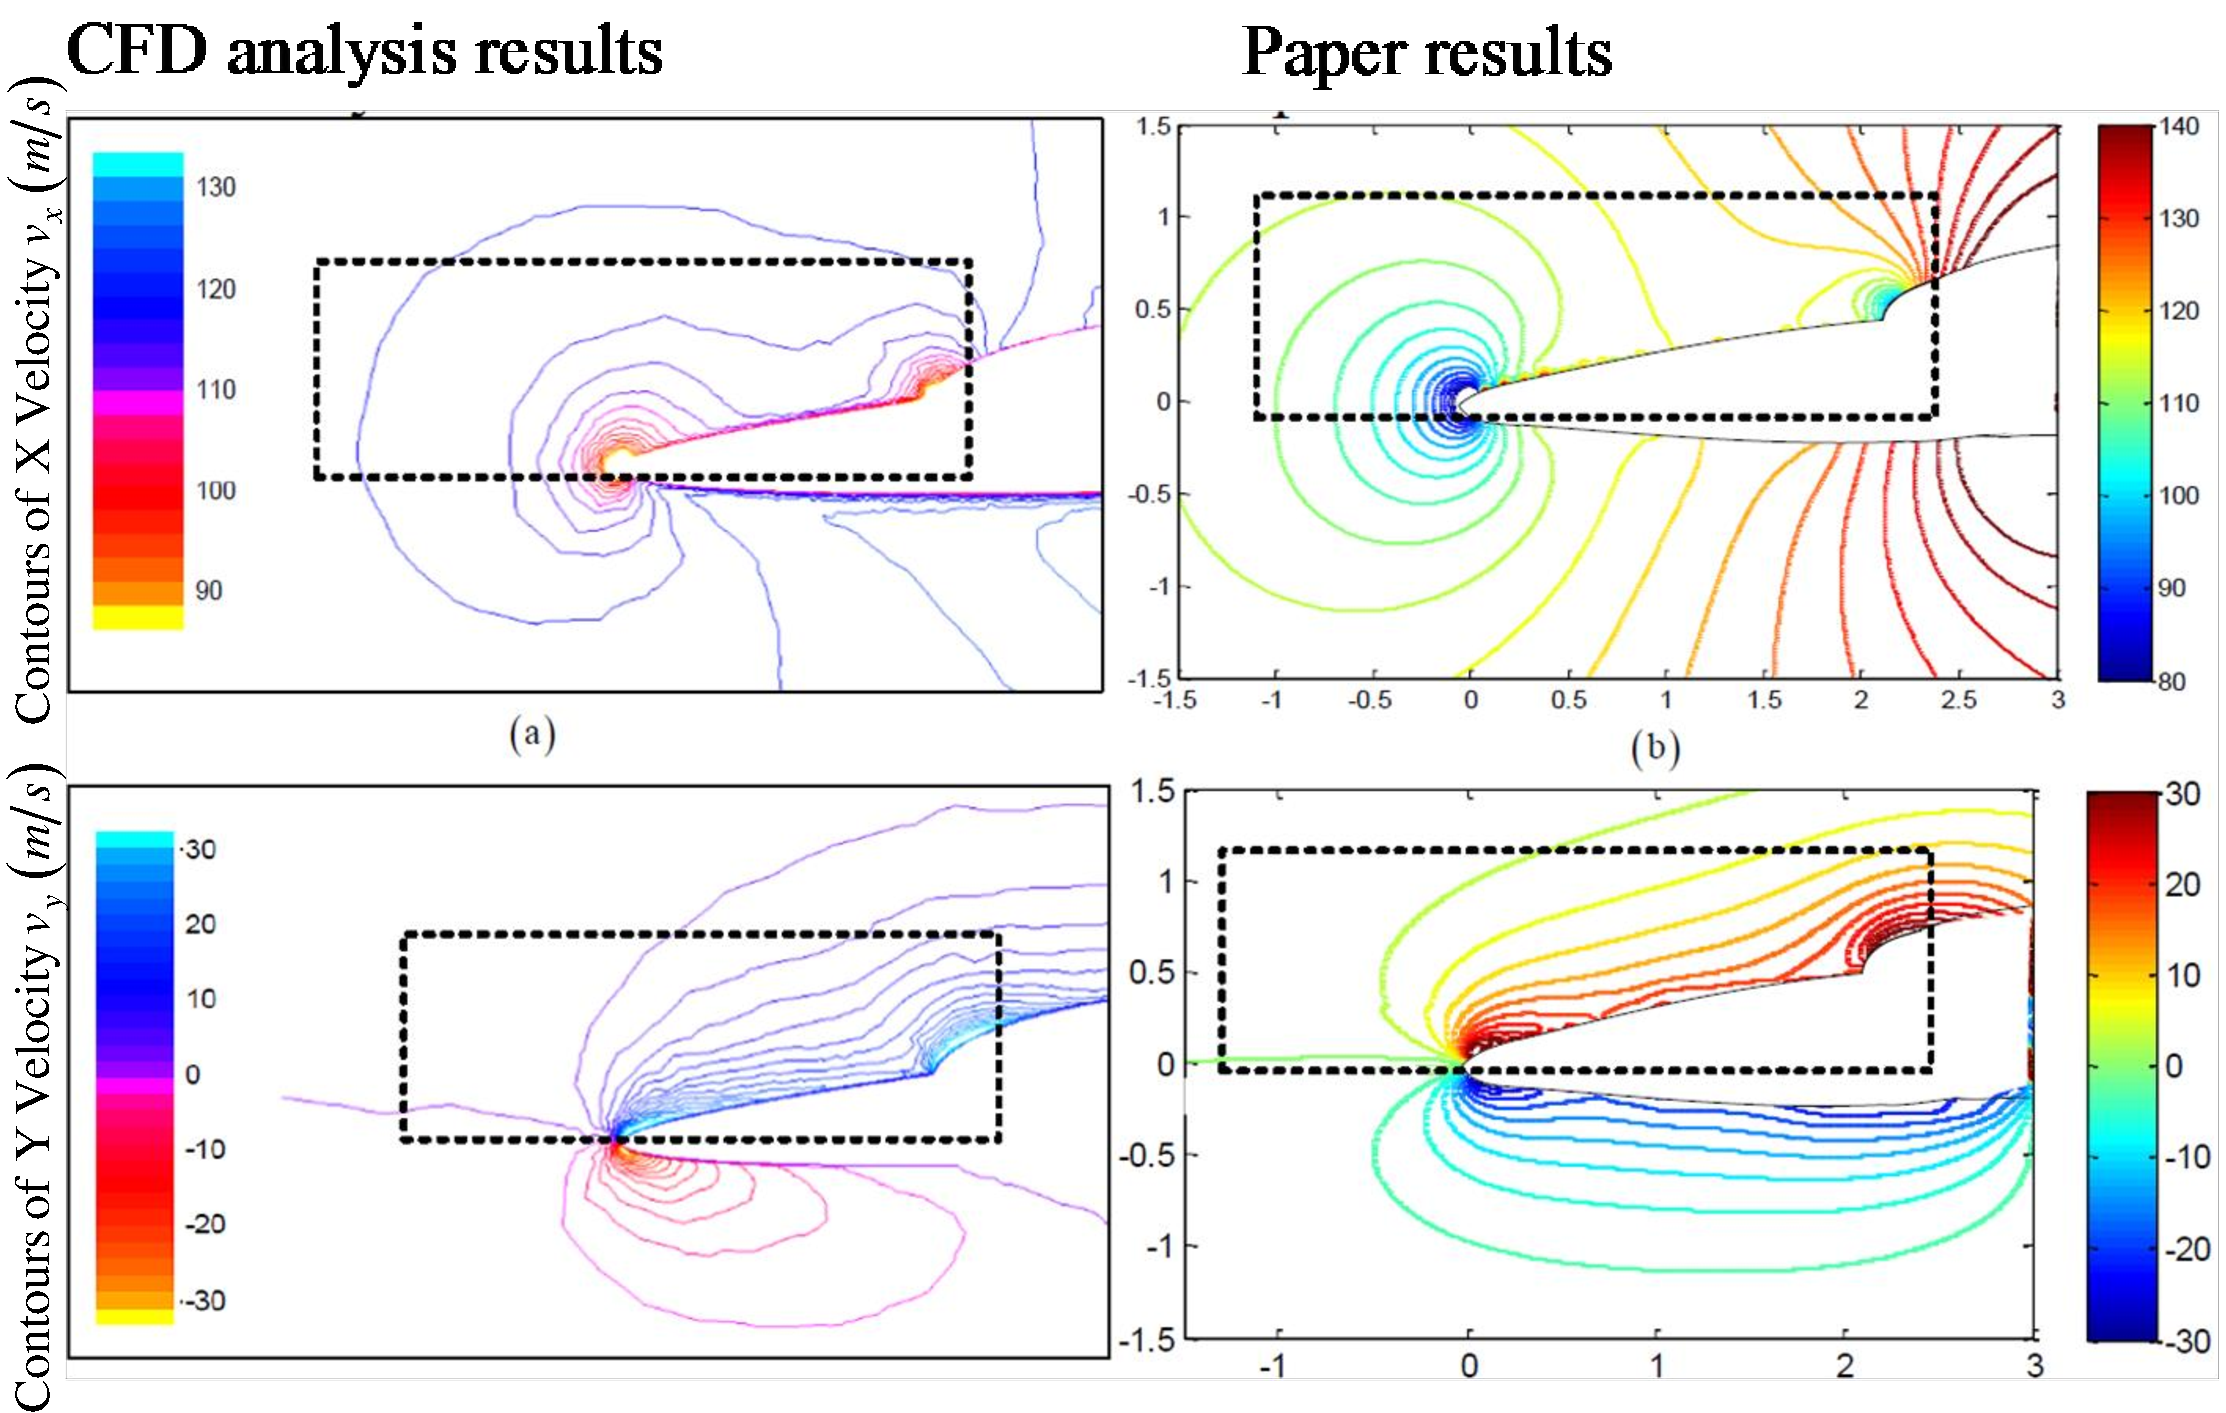
\includegraphics[width=0.7\textwidth]{Figures/Figs_Ch4/fig8.pdf}
	\caption{Validation of the stream function approach to model the bow wave flow field}\label{fig8}
\end{figure}
\subsection{Establishment of three-dimensional flow field of the aircraft nose}
Since the nose is usually a conical or ellipsoidal shape, rotationally symmetric about the center axis. Therefore, when the flow field of the nose profile is acquired, the profile two-dimensional flow field can be mapped to three-dimensional according to the method of rotational mapping as shown in Fig. \ref{fig9}. Specifically, the nose vertex is taken as the origin to establish the three-dimensional stream function coordinate system $o-xyz$, whose direction is the same as the direction of the receiver aircraft body coordinate system. 
\begin{figure}[th]
	\centering
	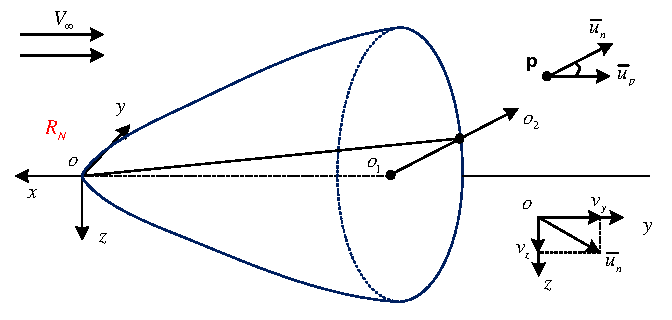
\includegraphics[width=0.6\textwidth]{Figures/Figs_Ch4/fig9.pdf}
	\caption{Schematic figure of the mapping of the two-dimensional flow field of the profile to three-dimensional flow field}\label{fig9}
\end{figure}\noindent
For the $\mathbf{p}$ with coordinates $(x,y,z)$ in the stream function coordinate system, the coordinates of its projection in the radial plane $oo_1o_2$ are $(x_p,y_p)$. The radial plane $oo_1o_2$ defined here corresponds to the two-dimensional stream function coordinate system defined in Fig. \ref{fig4}, and the mapping relationship between the two-dimensional coordinates and three-dimensional coordinates is as follows
\begin{equation}\label{eq36}
\left\{\begin{array}{l}
x_p=-x \\
y_p=\sqrt{y^2+z^2}
\end{array}\right.\, .
\end{equation}
According to Eq. (\ref{eq33}) and Eq. (\ref{eq34}), the two-dimensional modified velocity vector ${\left[{\begin{array}{*{20}{c}}{{{\bar u}_p}}&{{{\bar u}_n}}\end{array}} \right]^\mathrm{T}}$ at the point $\left( {{x_p},{y_p}} \right)$ can be obtained, and then by decomposing ${\bar u_p}$ and ${\bar u_n}$ in the three directional axes of the three-dimensional stream function coordinate system $o-xyz$, the three-dimensional velocity vector ${\mathbf{v}_\mathrm{B}} = {\left[ {\begin{array}{*{20}{c}}{{u_\mathrm{B}}}&{{v_\mathrm{B}}}&{{w_\mathrm{B}}}\end{array}} \right]^\mathrm{T}}$ can be obtained, which is denoted by
\begin{equation}\label{eq37}
\left\{\begin{array}{l}
u_{\mathrm{B}}=-\bar{u}_p\left(x_p, y_p\right) \\
v_{\mathrm{B}}=\frac{y}{\sqrt{y^2+z^2}} \bar{u}_n\left(x_p, y_p\right) \\
w_{\mathrm{B}}=\frac{z}{\sqrt{y^2+z^2}} \bar{u}_n\left(x_p, y_p\right)
\end{array}\right.
\end{equation}

The above coordinate mapping method applies to the case where the cross-section of the nose of the receiver aircraft is circular, but for most of the receiver aircraft, such as the F-16, the cross-section of the nose is approximated to be elliptical. Therefore, a scale change is first needed to transform the ellipse into a circle. As shown in Fig. \ref{fig10}, an ellipse in the $xyz$ plane with a long axis radius of $b$ and a short axis radius of $a$ is mapped to a circle with a radius of $a$ in the $oy'z'$ plane. The scale transformation relationship between the two coordinate systems can be expressed as
\begin{equation}\label{eq38}
x^{\prime}=x, y^{\prime}=\frac{a}{b} y, z^{\prime}=z
\end{equation}
By substituting the converted coordinates $\left( {x',y',z'} \right)$ into Eqs. (\ref{eq36}) and (\ref{eq37}), the three-dimensional velocity vector ${\mathbf{v'}_\mathrm{B}} ={\left[{\begin{array}{*{20}{c}}{{{u'}_\mathrm{B}}}&{{{v'}_\mathrm{B}}}&{{{w'}_\mathrm{B}}}\end{array}} \right]^\mathrm{T}}$ can be obtained, and then the coordinate inverse transformation is performed to obtain the velocity component under the original coordinate system 
\begin{equation}\label{eq39}
v_x=v_x^{\prime}, v_y=\frac{b}{a} v_y^{\prime}, v_z=v_z^{\prime}
\end{equation}
Thus, the three-dimensional velocity vector with elliptical cross-section ${\mathbf{v}_\mathrm{B}}={\left[{\begin{array}{*{20}{c}}{{u_\mathrm{B}}}&{{v_\mathrm{B}}}&{{w_\mathrm{B}}}\end{array}} \right]^\mathrm{T}}$ can be obtained. It is worth noting that, since the three-dimensional stream function coordinate system $o-xyz$ is in the same direction as the receiver aircraft body coordinate system, it satisfies $\mathbf{v}_\mathrm{B}^\mathrm{b}=\mathbf{v}_\mathrm{B}$, namely, the three-dimensional velocity vector obtained by this method is the induced velocity generated by the bow wave effect in the receiver body coordinate system.
\begin{figure}[th]
	\centering
	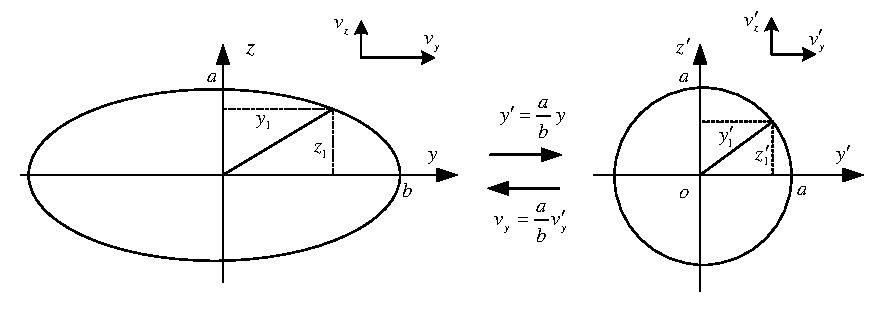
\includegraphics[width=0.9\textwidth]{Figures/Figs_Ch4/fig10.pdf}
	\caption{Scale transformation from ellipse to circle}\label{fig10}
\end{figure}

When the drogue enters the flow field range of the bow wave, it can be seen from the simulation results of CFD in Fig. \ref{fig8} that the flow field around the nose is drastically changing, which means that the flow velocity corresponding to different positions of the drogue is different. To solve this problem, an averaging method as shown in Fig. \ref{fig11} is used\cite{dogan2008flight}.
\begin{figure}[th]
	\centering
	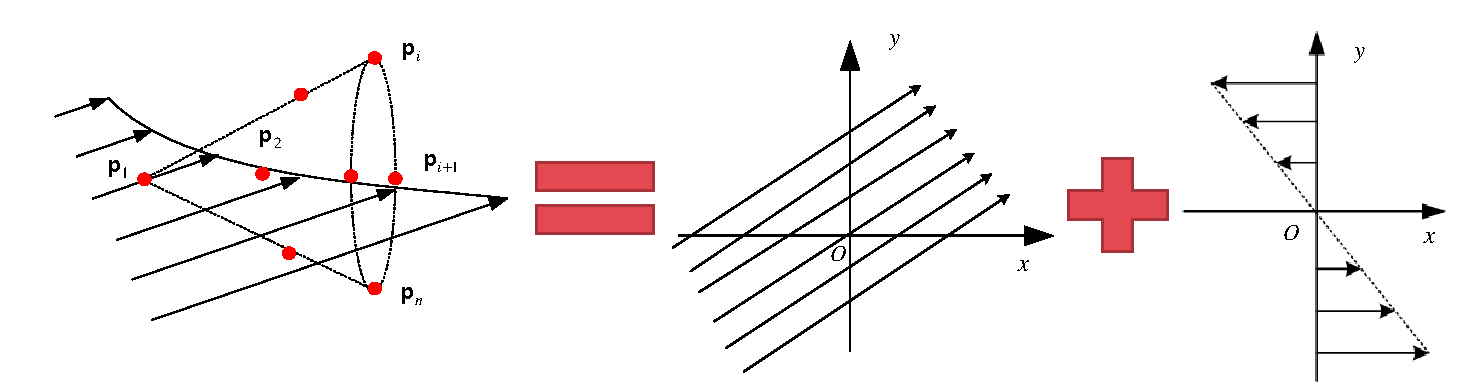
\includegraphics[width=1.0\textwidth]{Figures/Figs_Ch4/fig11.pdf}
	\caption{The flow field of the drogue is averaged into a uniform wind field with uniform rotation}\label{fig11}
\end{figure}

Sample the wind field at $n$ key points on the drogue  $\mathbf{v}_\mathrm{B}\left({{\mathbf{p}_i}} \right)$, and then by using the averaging method, the non-uniform wind field in which the drogue is located can be transformed to a constant (constant size and direction) wind field, and a rotating wind field. Due to the small size of the drogue, the induced moments generated by the rotating wind field are negligible. Therefore, the averaging algorithm can be expressed as
\begin{equation}\label{eq40}
\overline{\mathbf{v}}_{\mathrm{B}}^{\mathrm{b}}=\frac{1}{n} \sum_{i=1}^n \mathbf{v}_{\mathrm{B}}\left(\mathbf{p}_i\right)
\end{equation}

Assuming that the effects of atmospheric turbulence, wind gust, wind shear and the effect on the drogue of the perturbation velocity generated by the tanker wake are not taken into account in the body coordinate system, the velocity of the drogue with respect to the surrounding air $\mathbf{v}_{{\mathrm{d}\mathord{\left/{\vphantom {d w}} \right.\kern-\nulldelimiterspace} \mathrm{w}}}^\mathrm{b}$ can be expressed as
\begin{equation}\label{eq41}
\mathbf{v}_{\mathrm{d} / \mathrm{w}}^{\mathrm{b}}=\mathbf{v}_{\infty}+\overline{\mathbf{v}}_{\mathrm{B}}^{\mathrm{b}}
\end{equation}
where $\mathbf{v}_\infty={\left[{\begin{array}{*{20}{c}}{ - {V_\infty}}&0&0\end{array}} \right]^\mathrm{T}}$ represents the free stream velocity vector, which meets the relation $\mathbf{v}_\infty=-\mathbf{v}_\mathrm{r}$ with the receiver airspeed vector $\mathbf{v}_\mathrm{r}$, and the negative sign indicates the opposite direction. If $\mathbf{v}_{{\mathrm{d}\mathord{\left/{\vphantom {d w}} \right.\kern-\nulldelimiterspace} \mathrm{w}}}^\mathrm{b} = {\left[{\begin{array}{*{20}{c}}{{u_\mathrm{d}}}&{{v_\mathrm{d}}}&{{w_\mathrm{d}}}
		\end{array}} \right]^\mathrm{T}}$ is used, then the airspeed of the drogue $V_\mathrm{d}$, the attack angle $\alpha_\mathrm{d}$ and the side slip angle $\beta_\mathrm{d}$ can be expressed as follows
\begin{equation}\label{eq42}
\left\{\begin{array}{l}
V_{\mathrm{d}}=\sqrt{u_{\mathrm{d}}^2+v_{\mathrm{d}}^2+w_{\mathrm{d}}^2} \\
\alpha_{\mathrm{d}}=\tan ^{-1}\left(\frac{v_{\mathrm{d}}}{u_{\mathrm{d}}}\right) \\
\beta_{\mathrm{d}}=\sin ^{-1}\left(\frac{v_{\mathrm{d}}}{V_{\mathrm{d}}}\right)
\end{array}\right.
\end{equation}

After obtaining the velocity of the drogue relative to the surrounding air, the aerodynamic force on the drogue can be solved by using the same methods as that of the aerodynamic modeling of aircraft. The aerodynamic force on the drogue can be equivalent to an equation related to the dynamic pressure (the flow velocity is related to the air density), the windward area, and the aerodynamic coefficient, either by wind tunnel testing or computational fluid dynamics. In this case, the aerodynamic coefficient of the drogue can be expressed as follows, based on the symmetrical characteristics of the drogue
\begin{equation}\label{eq43}
\left\{\begin{array}{l}
C_{\mathrm{d} X}\left(\alpha_{\mathrm{d}}, \beta_{\mathrm{d}}\right)=C_{\mathrm{d} X_0}+C_{\mathrm{d} X_\alpha} \alpha_{\mathrm{d}}^2+C_{\mathrm{d} X_\beta} \beta_{\mathrm{d}}^2 \\
C_{\mathrm{d} Y}\left(\beta_{\mathrm{d}}\right)=C_{\mathrm{d} Y_\beta} \beta_{\mathrm{d}} \\
C_{\mathrm{d} Z}\left(\alpha_{\mathrm{d}}\right)=C_{\mathrm{d} Z_\alpha} \alpha_{\mathrm{d}}
\end{array}\right.
\end{equation}
where $C_{\mathrm{d} X}$, $C_{\mathrm{d} Y}$, $C_{\mathrm{d} Z}$ denote the aerodynamic coefficients of the drogue defined along the body, and $C_{\mathrm{d} X_0}$, $C_{\mathrm{d} X_\alpha}$, $C_{\mathrm{d} X_\beta}$, $C_{\mathrm{d} Y_\beta}$ and $C_{\mathrm{d} Z_\alpha}$ are the drogue coefficients, respectively, which need to be obtained by CFD simulation or wind tunnel testing.

\subsection{Derivation and validation of the force model for the drogue}
Using the method of aerodynamic coefficients commonly used in aircraft modeling, the final force on the drogue can be expressed as follows when only the bow wave effect is taken into account (if other perturbations are considered, a modification of Eq. (\ref{eq41}) is sufficient), the final force on the drogue can be expressed as
\begin{equation}\label{eq44}
\mathbf{F}_{\mathrm{d}}=\boldsymbol{f}_{\mathrm{d}}\left(\rho, \mathbf{v}_{\mathrm{d} / \mathrm{w}}^{\mathrm{b}}\right)=\frac{1}{2} \rho V_{\mathrm{d}}^2 S_{\mathrm{d}} \mathbf{C}_{\mathrm{d}}
\end{equation}
where ${V_\mathrm{d}}$ is the magnitude of the airspeed of the drogue, $S_\mathrm{d}$ is the reference area of the drogue, $\rho$ is the air density, and ${\mathbf{C}_\mathrm{d}} = {\left[ {\begin{array}{*{20}{c}}{{C_\mathrm{d}}_X\left( {{\alpha _\mathrm{d}},{\beta _\mathrm{d}}} \right)}&{{C_\mathrm{d}}_Y\left( {{\beta _\mathrm{d}}} \right)}&{{C_\mathrm{d}}_Z\left( {{\alpha _\mathrm{d}}} \right)}\end{array}} \right]^\mathrm{T}}$ is the matrix of aerodynamic parameters of the drogue, which is defined with reference to the aerodynamic parameters of the aircraft, and the measurements can be obtained using wind tunnel or CFD simulation.

Let $\mathbf{v}_{{\mathrm{d} \mathord{\left/{\vphantom {d w}} \right.\kern-\nulldelimiterspace}\mathrm{w}}}^\mathrm{b} = \mathbf{v}_\infty ^\mathrm{b} = {\left[ {\begin{array}{*{20}{c}}{ - {V_\infty }}&0&0\end{array}} \right]^\mathrm{T}}$, namely, without considering the bow wave effect, the force on the drogue can be expressed as
\begin{equation}\label{eq45}
\mathbf{F}_{\mathrm{d} 0}=\boldsymbol{f}_{\mathrm{d}}\left(\rho, \mathbf{v}_{\infty}\right)=\frac{1}{2} \rho V_{\infty}^2 S_{\mathrm{d}} \mathbf{C}_{\mathrm{d} 0}
\end{equation}
where ${\mathbf{C}_\mathrm{d0}} = {\left[ {\begin{array}{*{20}{c}}{{C_\mathrm{d}}_{{X_0}}}&0&0\end{array}} \right]^\mathrm{T}}$. Thus, the induced force on the drogue due to the bow wave effect alone can be obtained as
\begin{equation}\label{eq46}
\Delta \mathbf{F}_{\mathrm{d}}=\left[\begin{array}{c}
\Delta F_{\mathrm{d} X} \\
\Delta F_{\mathrm{d} Y} \\
\Delta F_{\mathrm{d} Z}
\end{array}\right]=\mathbf{F}_{\mathrm{d}}-\mathbf{F}_{\mathrm{d} 0}=\frac{1}{2} \rho V_{\mathrm{d}}^2 S_{\mathrm{d}}\left[\begin{array}{c}
C_{\mathrm{d} X}\left(\alpha_{\mathrm{d}}, \beta_{\mathrm{d}}\right) \\
C_{\mathrm{d} Y}\left(\beta_{\mathrm{d}}\right) \\
C_{\mathrm{d} Z}\left(\alpha_{\mathrm{d}}\right)
\end{array}\right]-\frac{1}{2} \rho V_{\infty}^2 S_{\mathrm{d}}\left[\begin{array}{c}
C_{\mathrm{d} X_0} \\
0 \\
0
\end{array}\right]
\end{equation}

After simulation verification. Through comparing the induced force generated by the bow wave effect on the drogue (Fig. \ref{fig12} right) with the CFD simulation results (Fig. \ref{fig12} left), it can be concluded that the modeling of the bow wave effect using this method has a high accuracy.

\section{Bow Wave Effect Model Based on link-connected model}
In Section 3.4, an analysis of "bow wave" has been done from the perspective of flow field theory. The bow wave model was first established, which refers to the flow field near the nose of the aircraft. Subsequently, the forces acting on the drogue in this flow field was analyzed. It is important to note that modeling the bow wave and modeling the bow wave effect are different concepts. The bow wave effect is essentially due to that the airflow changes after passing over the nose of the aircraft. The drogue swings in the changed flow field, and experiences a force similar to the repulsive force generated by the aircraft's nose. The term ``bow wave'' refers to the airflow that has passed over the aircraft's nose. Modeling the bow wave involves modeling the flow field of this airflow, which is unrelated to the drogue. On the other hand, the term "bow wave effect" pertains to the changes experienced by the drogue due to the bow wave. Essentially, modeling the bow wave effect involves capturing the disturbances affecting the drogue, such as modeling the forces acting on the drogue in the presence of the bow wave.

In this section, the bow wave effect will be analysed from a different perspective?directly modeling the bow wave effect without analyzing the flow field near the aircraft's nose. We begin by describing the bow wave effect and outlining the modeling steps. Subsequently, we divide the modeling process into two main parts: collecting Computational Fluid Dynamics (CFD) data and conducting multidimensional nonlinear fitting. Finally, we integrate the link-connected hose-drogue model to conduct simulations, analyze the bow wave effect, and further validate the model. Throughout this section, if no special instructions, lengths are in meters, and forces are in Newtons.
\subsection{Problem Description and Modeling Approach of the Bow Wave Effect Model}
First, the following assumptions are made.

Assumption 1: During the docking process, ${\bf{\Theta} _{\rm{r}}} \approx {\bf{0}}$.

Assumption 2: During the docking process, $ {{\mathbf{v}}}_{{\rm{r/w}}}^{\rm{g}} \approx  {{\mathbf{v}}}_{{\rm{t/w}}}^{\rm{g}}$.

For Assumption 1, since the tanker undergoes fine adjustments in attitude angles throughout the entire docking process to achieve position changes, the attitude angles of the tanker remain relatively small during the docking process. Therefore, it can be assumed that ${{\bf{\Theta}} _{\rm{r}}} \approx {\bf{0}}$ in this process, where ${{\bf{\Theta}} _{\rm{r}}} = {\left[ {\begin{array}{*{20}{c}}
		{{\theta _{\rm{r}}}}&{{\psi _{\rm{r}}}}&{{\phi _{\rm{r}}}}
		\end{array}} \right]^\mathrm{T}}$. Therefore, Assumption 1 holds.

Regarding Assumption 2, its significance lies in considering that the receiver's airspeed is equal to the tanker's airspeed during the docking process, and remains unchanged. This is because the relative velocity between the receiver and the tanker is significantly lower compared to the velocity of the tanker. Therefore, Assumption 2 holds.

\subsubsection{Problem Description of the Bow Wave Effect Model}
The influence of the bow wave effect extends approximately from a short distance in front of the aircraft's nose. In other words, the range of the bow wave effect is relatively short. Therefore, it can be considered that it only affects the drogue and doesn't exert any aerodynamic influence on the hose. Based on the modeling of the refueling equipment described in Section 4.2, we can use the following equation to describe the bow wave effect 
\begin{equation}\label{eq4.99}
\left\{ \begin{aligned}
&{{ {\dot {\bf{x}}}}_{\rm{h}}} = { {{\bm{f}}}_{{\rm{h0}}}}\left( {{ {{\bf{x}}}_{\rm{h}}},{ {{\bf{x}}}_{\rm{d}}},\mathbf {v}_{{\rm{t/w}}}^{\rm{g}},h_{\rm{t}}^{\rm{g}}} \right)\\
&{{ {\dot {\bf{x}}}}_{\rm{d}}} = { {{\bm{f}}}_{{\rm{d0}}}}\left( {{ {{\bf{x}}}_{\rm{h}}},{ {{\bf{x}}}_{\rm{d}}},\mathbf {v}_{{\rm{t/w}}}^{\rm{g}},h_{\rm{t}}^{\rm{g}},{ {{\mathbf{F}}}_{\rm{b}}}} \right)\\
&{ {{\bf{p}}}_{\rm{d}}} = { {{\bm{f}}}_y}\left( {{ {{\bf{x}}}_{\rm{h}}},{ {{\bf{x}}}_{\rm{d}}}} \right)
\end{aligned} \right.
\end{equation}
Here, the functions ${ {{\bm{f}}}_{{\rm{h0}}}}, { {{\bm{f}}}_{{\rm{d0}}}}$ and ${ {{\bm{f}}}_y}$ are formed by the link-connected hose-drogue model. The variables ${ {{\mathbf{x}}}_{\rm{h}}}$ and ${ {{\mathbf{x}}}_{\rm{d}}}$ represent the state variables composed of the directional angles and angular velocities of each link. The output is the position ${ \mathbf{p}_{\rm{d}}}$ of the drogue in the tanker's coordinate system. The input to this system is the force ${ {{\mathbf{F}}}_{\rm{b}}} \in \mathbb{R}^{3}$ exerted on the drogue due to the bow wave effect.

Based on experience, ${ \mathbf{F}_{\rm{b}}}$ is expected to be a force generated by the relative states between the tanker and the drogue. The bow wave effect aims to discuss the relationship between ${ {{\mathbf{F}}}_{\rm{b}}}$, the tanker, and the drogue, as well as the dynamic behavior of the drogue under the influence of ${ {{\mathbf{F}}}_{\rm{b}}}$.

Firstly, it can be inferred that ${ {{\mathbf{F}}}_{\rm{b}}}$ is mainly related to the position of the drogue ${{\bf{p}}}_{\rm{d}}^{\rm{r}}$ in the coordinate frame of the receiver and the receiver's airspeed ${{\mathbf{v}}}_{{\rm{r/w}}}^{\rm{g}}$. It can be expressed as 
\begin{equation}\label{eq4.100}
{ {{\mathbf{F}}}_{\rm{b}}} = {\bf{R}}_{{\rm{r/t}}}^{\rm{T}}\left( {{ {\theta }_{\rm{r}}}} \right) {{\mathbf{F}}}_{\rm{b}}^{\rm{r}} = {\bf{R}}_{{\rm{r/t}}}^{\rm{T}}\left( {{ {\theta }_{\rm{r}}}} \right){ {{\bm{f}}}_{{\rm{b1}}}}\left( { {{\bf{p}}}_{\rm{d}}^{\rm{r}}, {{\mathbf{v}}}_{{\rm{r/w}}}^{\rm{g}}} \right)
\end{equation}
The above equation represents the model for the bow wave effect. According to Assumption 2, one have 
\begin{equation}\label{eq4.101}
{ {{\mathbf{F}}}_{\rm{b}}} = { {{\bm{f}}}_{{\rm{b2}}}}\left( { {{\bf{p}}}_{\rm{d}}^{\rm{r}}} \right)
\end{equation}
where ${ {{\bm{f}}}_{{\rm{b2}}}}\left( { {{\bf{p}}}_{\rm{d}}^{\rm{r}}} \right)\triangleq { {{\bm{f}}}_{{\rm{b}}1}}\left( { {{\bf{p}}}_{\rm{d}}^{\rm{r}}, {{\mathbf{v}}}_{{\rm{t/w}}}^{\rm{g}}} \right)$. The utilization of Assumption 2 in this context is consistent with the actual situation:

(1) The reason for the correlation between the function relationship ${ {{\bm{f}}}_{{\rm{b1}}}}$ and $ {{\mathbf{v}}}_{{\rm{r/w}}}^{\rm{g}}$ is that the aerodynamic force generated by the bow wave is related to the airspeed of the receiver. However, the airspeed of the receiver can be expressed as 
\begin{equation}\label{eq4.102}
{{\mathbf{v}}}_{{\rm{r/w}}}^{\rm{g}} =  {{\mathbf{v}}}_{{\rm{r/t}}}^{\rm{g}} +  {{\mathbf{v}}}_{{\rm{t/w}}}^{\rm{g}}
\end{equation}
During the docking process, $ {{\mathbf{v}}}_{{\rm{r/t}}}^{\rm{g}} \ll  {{\mathbf{v}}}_{{\rm{t/w}}}^{\rm{g}}$, so it can be neglected, which means that $ {{\mathbf{v}}}_{{\rm{r/w}}}^{\rm{g}} \approx  {{\mathbf{v}}}_{{\rm{t/w}}}^{\rm{g}}$.

(2) According to the NATO AAR Manual \cite{vassberg_numerical_2003}, pilots have two approaches during the refueling process: the first one is a rapid approach, characterized by a larger ${ {{\mathbf{v}}}_{{\rm{r/t}}}}$, allowing for quick docking before the drogue deviates significantly from its equilibrium position due to the bow wave; the second approach involves estimating the drogue's deviation beforehand and executing a slow approach with a smaller ${ {{\mathbf{v}}}_{{\rm{r/t}}}}$. Although the first method enables docking before substantial drogue drift occurs, controlling the relative velocity for engaging the refueling valve can be challenging, potentially leading to refueling accidents. On the other hand, the second method may result in drogue drift but is considered safer. Due to the high-risk nature of aerial refueling, the manual deems the second approach more reasonable. This further explains the reasonableness of neglecting the effect of ${\bf {v}_{{\rm{r/t}}}}$ in practical operations.

On the other hand, in the process of modeling the bow wave effect, it is necessary to use CFD software to generate training data. In this process, the CFD coordinate system is made use of, which was briefly introduced in \textit{Chapter 2}. Therefore, ${{\bf{p}}}_{\rm{d}}^{\rm{r}}$ is transformed into this coordinate system 
\begin{equation}\label{eq4.103}
{{\bf{p}}}_{\rm{d}}^{\rm{r}} =  {{\bf{p}}}_{{\rm{d/r}}}^{\rm{r}} =  {{\bf{p}}}_{{\rm{d/f}}}^{\rm{r}} +  {{\bf{p}}}_{{\rm{f/r}}}^{\rm{r}} =  {{\bf{p}}}_{\rm{d}}^{\rm{f}} +  {{\bf{p}}}_{\rm{f}}^{\rm{r}}
\end{equation}
According to Assumption 1, it can be deduced that $ {{\bf{p}}}_{\rm{d}}^{\rm{f}}$ can also be expressed as 
\begin{equation}\label{eq4.104}
{{\bf{p}}}_{\rm{d}}^{\rm{f}} = { {{\bf{p}}}_{\rm{d}}} - { {{\bf{p}}}_{\rm{f}}}
\end{equation}
Therefore, the bow wave effect model can be further rewritten as 
\begin{equation}\label{eq4.105}
{ {{\mathbf{F}}}_{\rm{b}}} = { {{\bm{f}}}_{\rm{b}}}\left( { {{\bf{p}}}_{\rm{d}}^{\rm{f}}} \right)
\end{equation}
where ${ {{\bm{f}}}_{\rm{b}}}\left( { {{\bf{p}}}_{\rm{d}}^{\rm{f}}} \right) \triangleq { {{\bm{f}}}_{{\rm{b}}1}}\left( { {{\bf{p}}}_{\rm{d}}^{\rm{f}} { + {\bf{p}}}_{\rm{f}}^{\rm{r}}} \right)$.

Thus, based on Eq. (\ref{eq4.99}) and Eq. (\ref{eq4.105}), we can derive the relationship between the bow wave effect generated by the relative position of the tanker and drogue and the link-connected hose-drogue model, as shown in Fig. \ref{fig4.10}. Here, ${ {{\bf{p}}}_{\rm{r}}}\left( 0 \right)$ represents the initial position of the receiver in the tanker's coordinate system, and $\Delta { {{\bf{p}}}_{\rm{r}}}$ indicates the docking trajectory of the receiver relative to the initial position.
\begin{figure}[th]
	\centering
	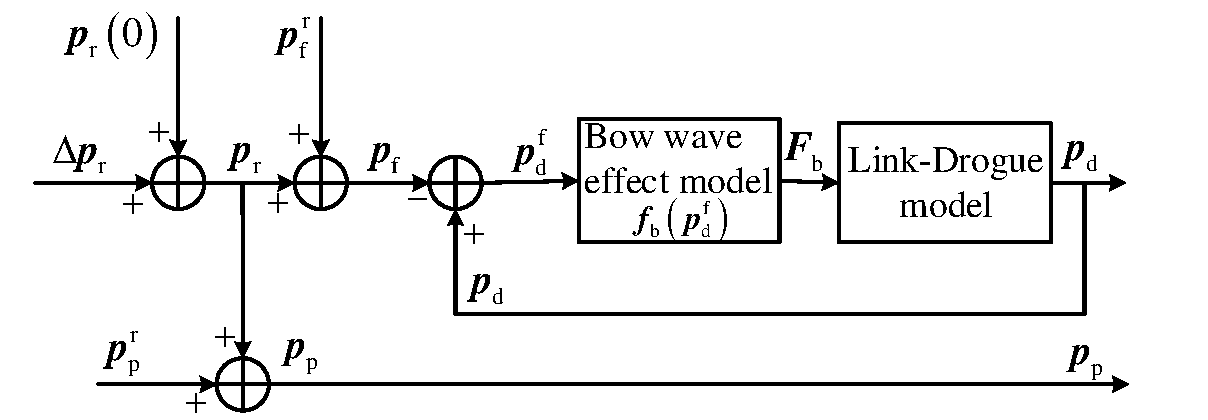
\includegraphics[width=0.7\textwidth]{Figures/Figs_Ch4/fig13.pdf}
	\caption{Relationship between Bow Wave Effect Model and link-connected hose-drogue model}\label{fig4.10}
\end{figure}
\subsubsection{Modeling Approach for the Bow Wave Effect Model}
There are mainly two methods for modeling the bow wave effect. One method is the approach introduced in Section 3.4, where the theoretical derivation is used to gradually approximate the distribution of the flow field using multiple dipoles. Although this method can provide a good approximation of the model, as the model's precision improves, the number of dipoles significantly increases, leading to a high number of model parameters and overall complexity. In this section, the modeling approach presented in Ref. \cite{wei_drogue_2016} is adopted. This approach involves the following five steps:

(1) Establish the CFD simulation environment and define its position in the receiver's coordinate system.

(2) Select spatial points within the primary operational region of the bow wave effect ${ {{\bm{f}}}_{\rm{b}}}\left( { {{\bf{p}}}_{\rm{d}}^{\rm{f}}} \right)$ and generate a large set of training data.

(3) Infer the functional form of the bow wave effect model with parameter estimations based on the profiles of the training data.

(4) Employ nonlinear regression to calculate the specific parameters in ${ {{\bm{f}}}_{\rm{b}}}\left( { {{\bf{p}}}_{\rm{d}}^{\rm{f}}} \right)$, resulting in a concrete bow wave effect model.

(5) Perform initial validation to assess the effectiveness of the parameters.

The first two steps belong to the CFD data acquisition phase, which will be elaborated in Section 4.3.2. The subsequent three steps are related to the bow wave effect model and parameter estimation, which will be discussed in Section 4.3.3. In Section 4.3.4, the obtained bow wave effect will be integrated with the link-connected hode-drogue model for the analysis of the bow wave effect. A comparison will also be made against a set of publicly available simulation and experimental data from the United States, providing further validation of the model's effectiveness.

Analyzing the bow wave effect using a mechanistic model involves two main steps. First, modeling the flow field generated by the bow wave formation, and then analyzing the aerodynamic coefficients of the drogue in this flow field to determine the resulting forces on the drogue. Due to the inherent complexity of the bow wave model itself and the irregular shape of the drogue with hollow features, it becomes challenging to establish a bow wave effect model directly from mechanistic principles. This approach, based on data and fitting methods, provides a way to bypass the complexity of this analysis and directly obtain a model for the bow wave effect.

The bow wave effect model established through this process exhibits a certain universality for aircraft with nose shapes resembling ellipsoids (such as F-16, J-8, etc.). However, the parameters within the model are influenced by factors like the shape parameters of the aircraft's nose, the aerodynamic parameters of the drogue, and the airspeed. This method requires a substantial amount of Computational Fluid Dynamics (CFD) data to derive a generalized functional form with a limited number of parameters. Consequently, when modeling for different scenarios, this model can be applied with relatively fewer data points. To achieve a more accurate model, wind tunnel testing can also be employed in the data collection phase. The limited parameter amount significantly reduces the workload required for simulation or experimentation.

\subsection{Collection of CFD Data for Bow Wave Effect}

\subsubsection{Establishment of CFD Simulation Environment}

(1) Creating a 3D Model

Fluent is utilized as the simulation software for Computational Fluid Dynamics (CFD). Initially, the object for analyzing the bow wave effect was established. Fig. \ref{fig4.11} (d) presents the 3D model constructed using Gambit, while Figs. \ref{fig4.11} (a)-(c) show its corresponding three views. The aircraft nose model was set with parameters resembling those of the F-16 nose. Fig. \ref{fig4.12} provides a detailed exhibit of the 3D model.

It is important to note that during the process of collecting CFD data, a substantial amount of data is required for subsequent extrapolation of the functional form and parameter calculation. Hence, it is essential to minimize computation while maintaining a certain level of accuracy. Therefore, in the 3D modeling, certain aspects that have minimal impact were deliberately omitted. Specifically, these include:

1) The rear part of the fuselage behind the nose was neglected. Since the bow wave effect is primarily a result of the airflow passing over the nose and affecting the drogue, the region generating the bow wave is mainly the nose. Additionally, the impact on the drogue is limited by the docking distance, and the rear part of the aircraft will not significantly affect the drogue. Hence, the portion behind the nose was omitted, significantly reducing the total grid count.
\begin{figure}[th]
	\centering
	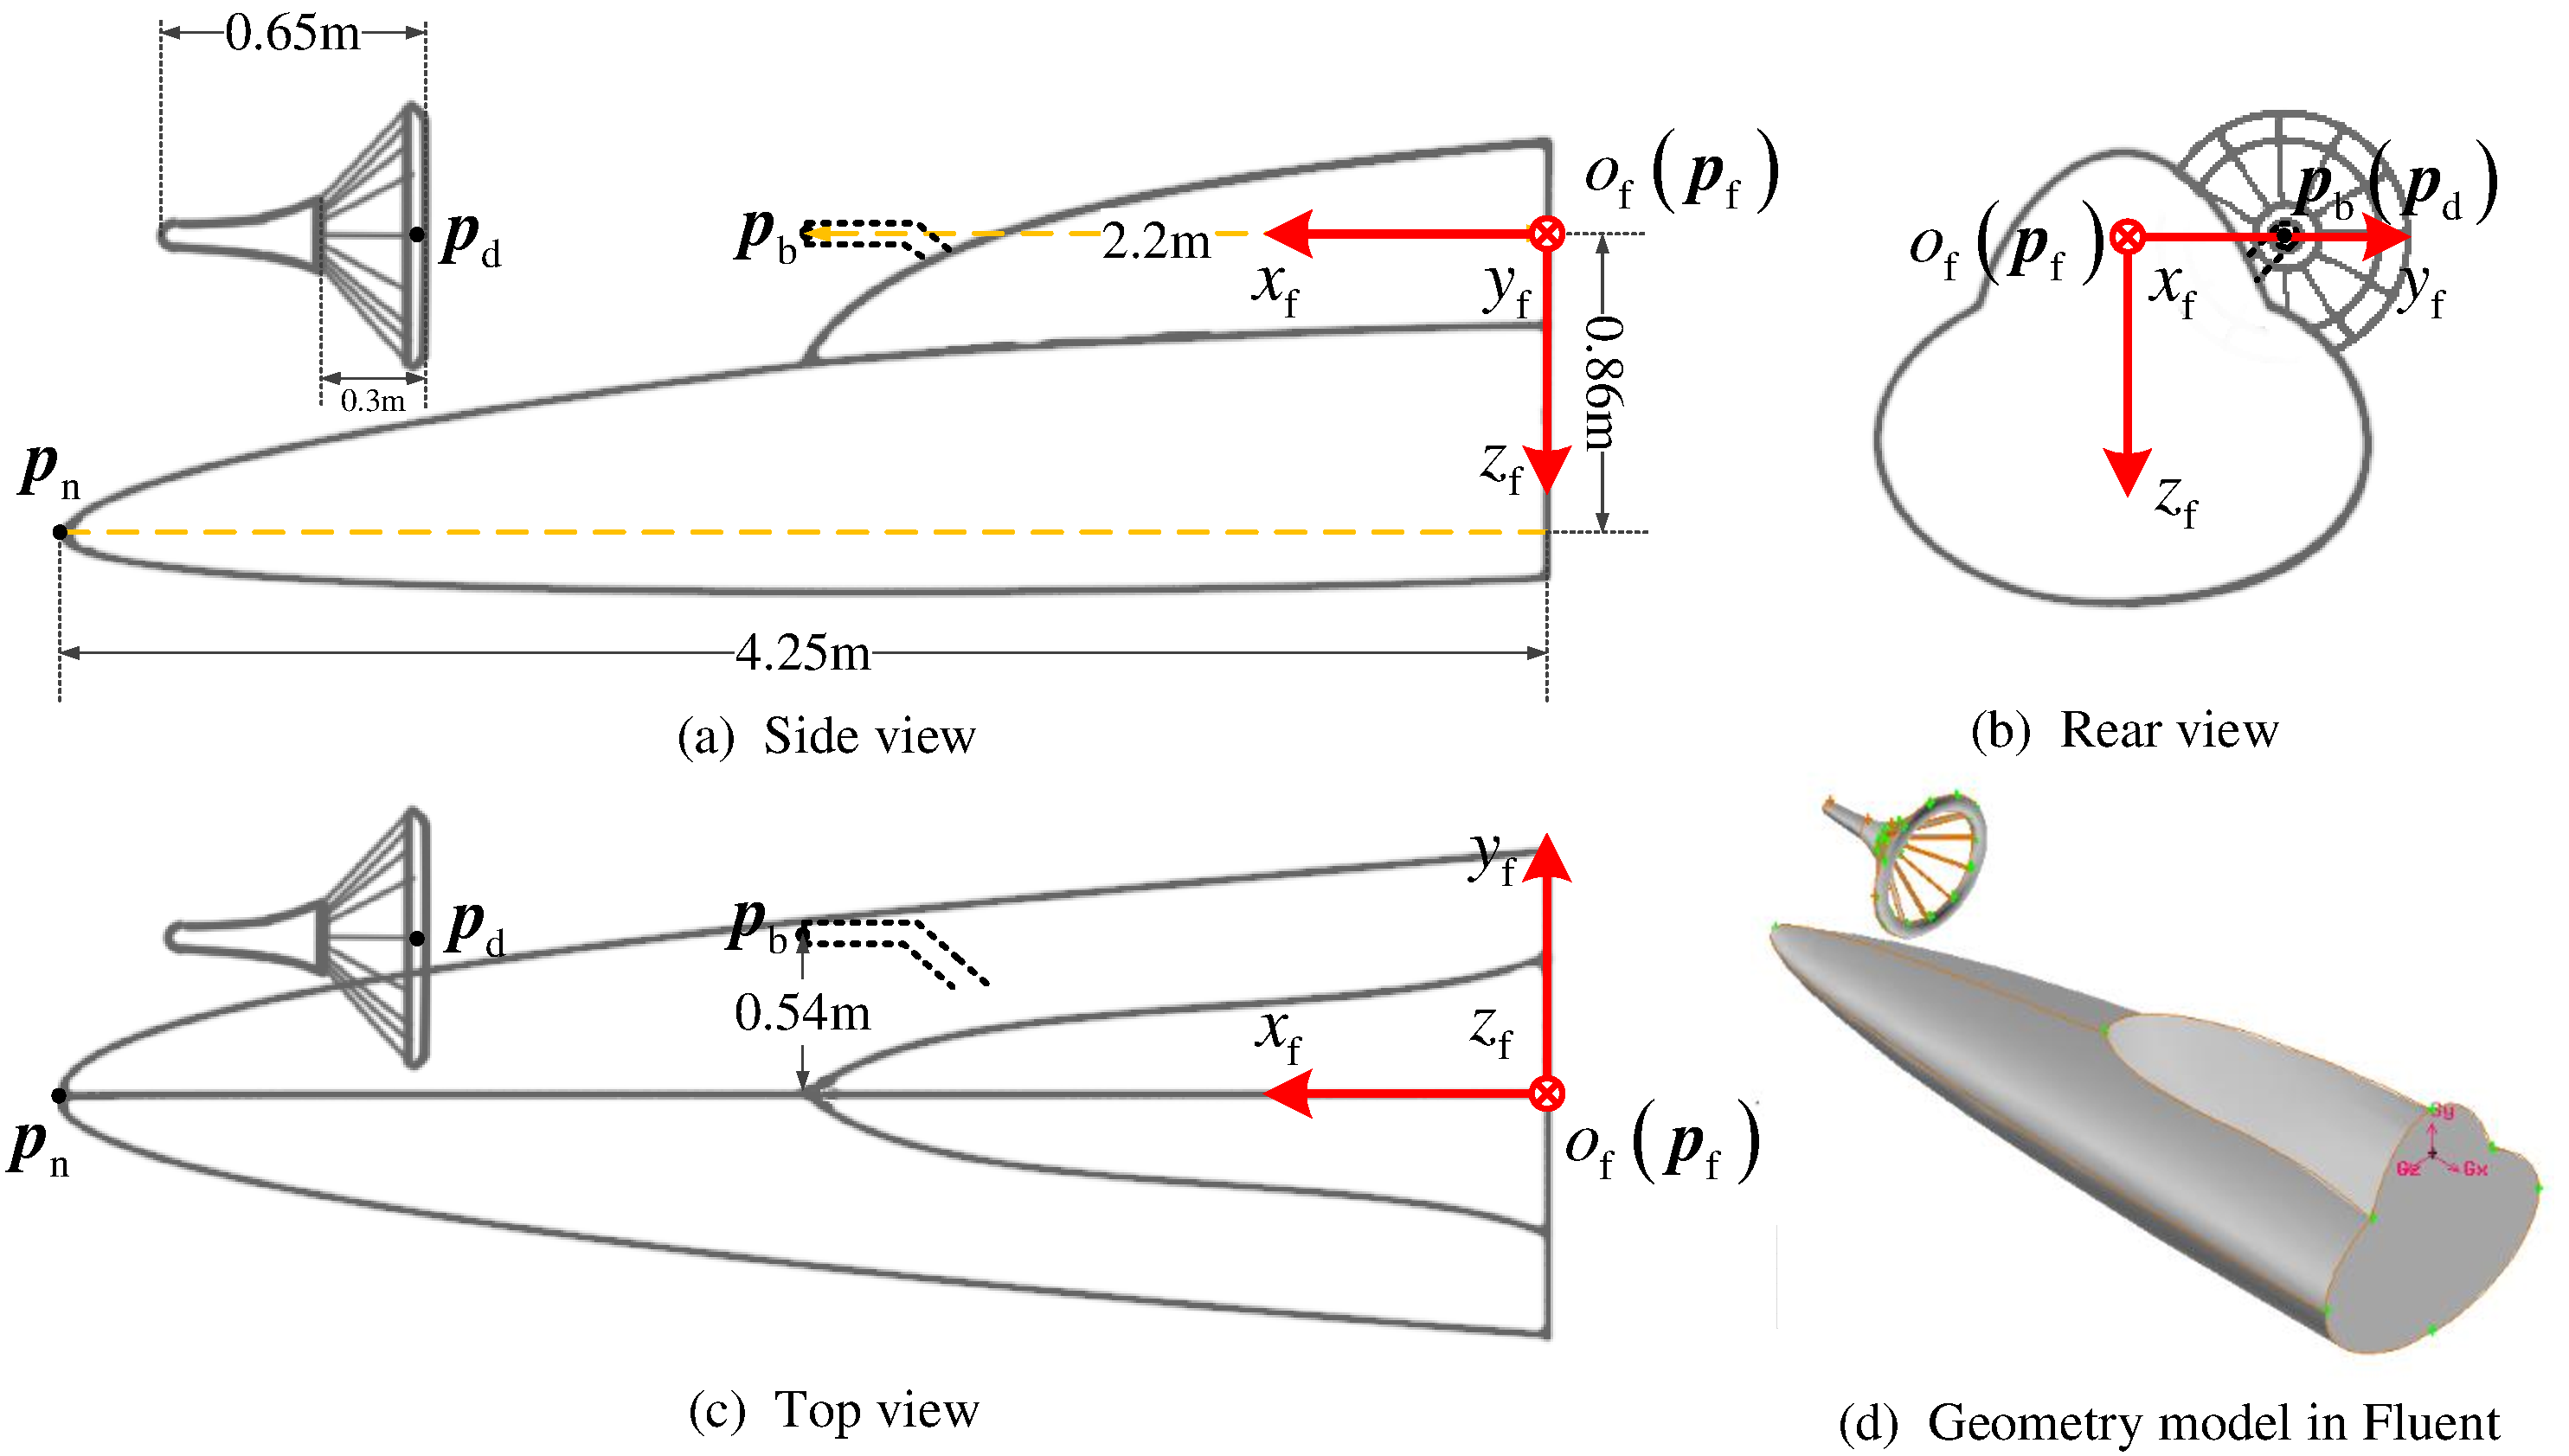
\includegraphics[width=0.7\textwidth]{Figures/Figs_Ch4/fig14.pdf}
	\caption{Three-dimensional Model in Fluent and its Three Views}\label{fig4.11}
\end{figure}
\begin{figure}[th]
	\centering
	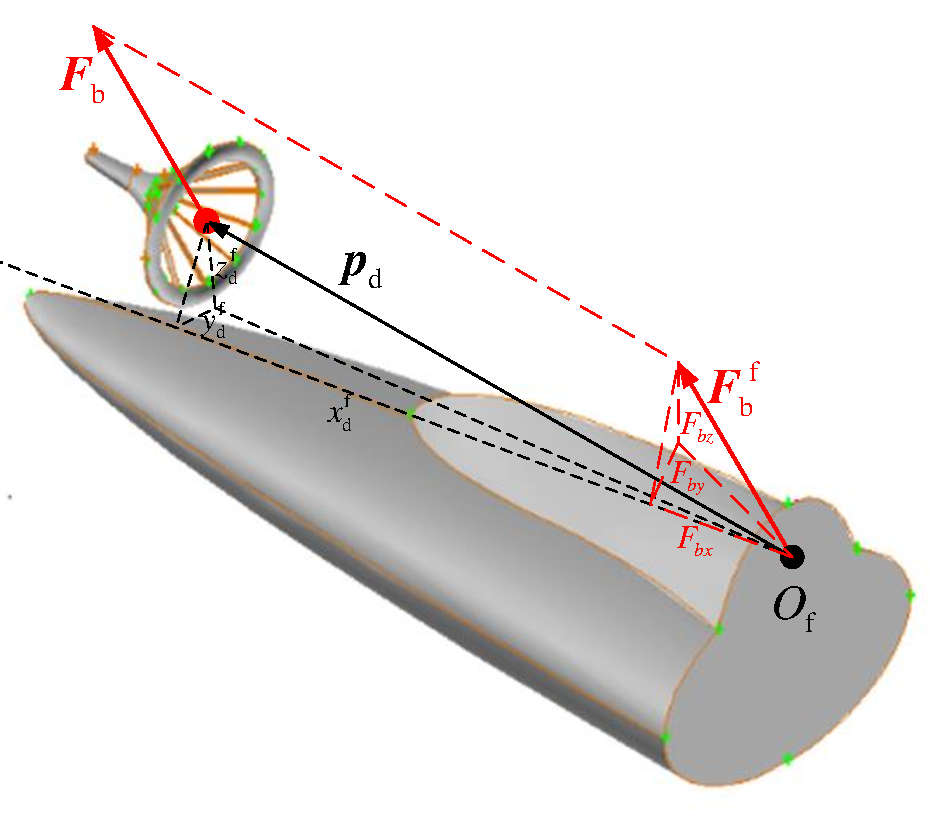
\includegraphics[width=0.6\textwidth]{Figures/Figs_Ch4/fig15.pdf}
	\caption{Details of the Three-dimensional Model}\label{fig4.12}
\end{figure}

2) The probe was neglected. From Fig. \ref{fig4.12}, it can be observed that the probe was actually excluded in the CFD simulation. Similar to the previous point, the bow wave caused by the probe (every object generates a bow wave) has a very limited impact distance. By the time the drogue enters the region affected by the probe's bow wave, the docking process is almost completed. Furthermore, the magnitude of the bow wave is influenced by the size of the object. Due to the small volume of the probe, the alteration in the bow wave it induces is minimal. Therefore, the probe's effect on the drogue is short in time and small in magnitude, allowing it to be disregarded.

3) The drogue's crown section was replaced with a rigid body. The crown of the drogue is actually a flexible structure with an opening. However, in flight, due to high-speed airflow, this part extends and behaves more like a rigid body. Using a rigid body to represent this flexible section simplifies the modeling process and reduces computational complexity. For readers seeking a more precise drogue modeling, Ref. \cite{ro_aerodynamic_2007} can be consulted.

4) The hose is disregarded. As explained in Section 4.3.1.1, this is due to the short range of the bow wave's influence. The impact on the hose can be ignored.

(2) Establishing a Coordinate System for CFD Simulation

Use the CFD coordinate system established in Section 2.2.5.

(3) Generation and Solving of Fluent Mesh

Create a cubic grid with dimensions of $10\text{m} \times 6\text{m} \times 6\text{m}$ around the aircraft and drogue, as illustrated in Fig. \ref{fig4.13}. This grid comprises approximately $2.6 \times {10^6}$ cells and is a hybrid mesh type. To achieve an appropriate grid density for obtaining higher accuracy data, the grid spacing on the surfaces of the drogue and aircraft is set to approximately $0.005\text{m}$. The length of these grid cells is around $1/20$ of the length of the edge grid cells. The k-epsilon turbulence model is employed for solving.
\begin{figure}[th]
	\centering
	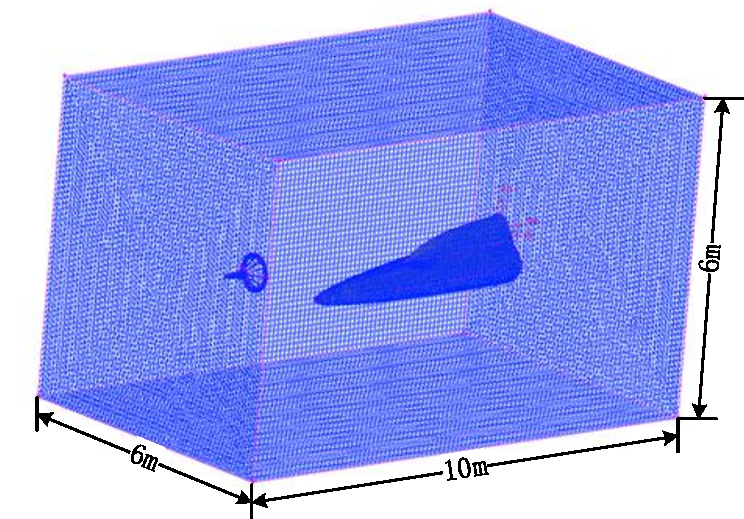
\includegraphics[width=0.7\textwidth]{Figures/Figs_Ch4/fig16.pdf}
	\caption{Mesh Generated in Fluent}\label{fig4.13}
\end{figure}

\subsubsection{Collection of CFD Data}

(1) Training Data

In the CFD simulation environment described in Section 4.3.2.1, change the relative positions of the drogue and aircraft to collect data. Each relative position corresponds to a position $ {{\bf{p}}}_{{\rm{d}},i}^{\rm{f}} = {\left[ {\begin{array}{*{20}{c}}
		{x_{{\rm{d}},i}^{\rm{f}}}&{y_{{\rm{d}},i}^{\rm{f}}}&{z_{{\rm{d}},i}^{\rm{f}}}
		\end{array}} \right]^{\rm{T}}}$ of the drogue in the CFD coordinate system. A simulation is performed using Fluent to calculate the corresponding force data ${ {{\mathbf{F}}}_{{\rm{b}},i}} = {\left[ {\begin{array}{*{20}{c}}
		{{F_{{\rm{b}}x,i}}}&{{F_{{\rm{b}}y,i}}}&{{F_{{\rm{b}}z,i}}}
		\end{array}} \right]^{\rm{T}}}$ acting on the drogue. According to Assumption 2 and the definition of the CFD coordinate system, it is known that ${ {{\mathbf{F}}}_{{\rm{b}},i}} =  {{\mathbf{F}}}_{{\rm{b}},i}^{\rm{f}}$. Hence, the force data ${ {{\mathbf{F}}}_{{\rm{b}},i}}$ is directly recorded in the tanker coordinate system. In this manner, for each relative position, the collected training data is represented as the $i$-th set $\left[ {\begin{array}{*{20}{c}}
	{ {{\bf{p}}}_{{\rm{d}},i}^{\rm{f}}}&{{ {{\mathbf{F}}}_{{\rm{b}},i}}}
	\end{array}} \right]$.

Taking the simulation at ${{\bf{p}}}_{{\rm{d}},i}^{\rm{f}} = {\left[ {\begin{array}{*{20}{c}}
		{3.5}&0&0
		\end{array}} \right]^{\rm{T}}}$ as an example, after performing the simulation using Fluent, analysis results such as the contour plot of fluid velocity magnitude, as shown in Fig. \ref{fig4.14}, can be obtained. Simultaneously, the force data acting on the drogue's mass center can be read as ${ {{\mathbf{F}}}_{{\rm{b}},i}} = {\left[ {\begin{array}{*{20}{c}}
		{82.5566}&{0.2014}&{41.0140}
		\end{array}} \right]^{\rm{T}}}$.

(2) Collection of Training Data

Over 200 training data points are collected from the region $ {{\bf{p}}}_{{\rm{d}},i}^{\rm{f}} \in \left[ {2,6} \right] \times \left[ { - 2,2} \right] \times \left[ { - 0.5,0.1} \right]$. The reason for choosing this region is that, during the docking process, the drogue primarily operates within the region affected by the bow wave. All the training data has been provided in the Appendix of Section 4.3.5 of this chapter.
\begin{figure}[th]
	\centering
	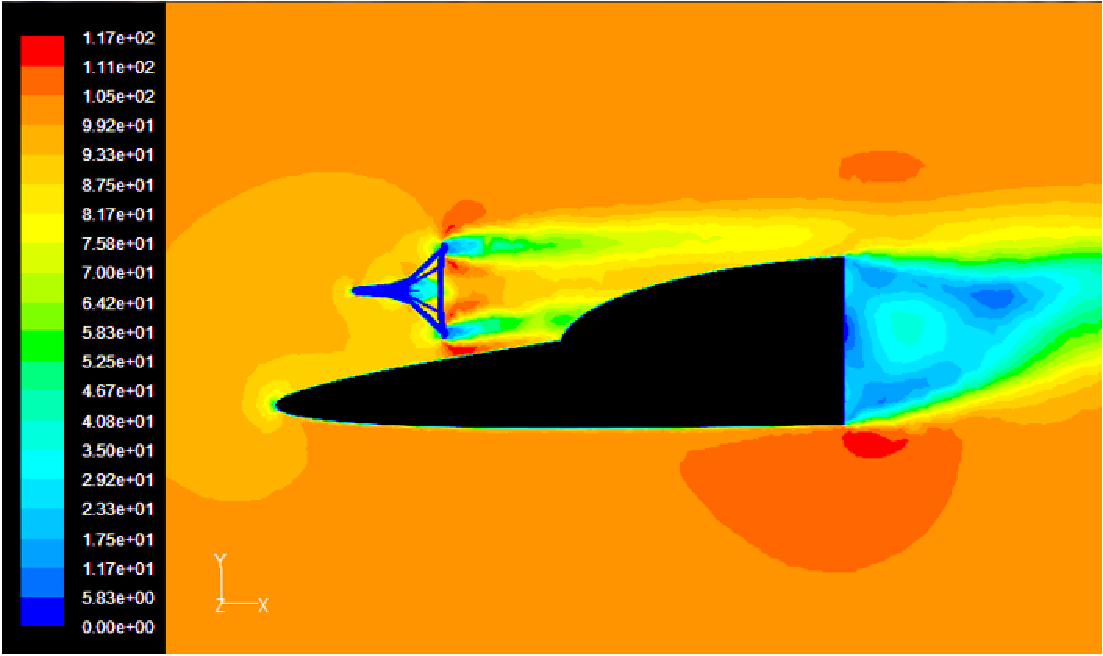
\includegraphics[width=0.7\textwidth]{Figures/Figs_Ch4/fig17.pdf}
	\caption {Contour Plot of Fluid Velocity Magnitude when ${{\bf{p}}}_{{\rm{d}},i}^{\rm{f}}=\left[ { 3.5,0,0} \right]^{\rm{T}}$ } \label{fig4.14}
	
\end{figure}
It should be noted that the data directly collected from CFD needs to undergo certain processing before it can be used as training data:

1) The software's coordinate axis direction definition is different from ours, so the collected ${F_{{\rm{b}}z}}$ values need to be taken with the opposite sign to match the definition in the CFD coordinate system (indicated in the table header).

2) In the absence of bow wave disturbance, the drogue will also experience a force ${F_{{\rm{b}}x\infty }}$ in the ${o_{\rm{f}}}{x_{\rm{f}}}$ direction. The bow wave reduces this force, and Fluent provides the reduced force directly. Therefore, the actual training data should be obtained from ${F_{{\rm{b}}x}} = {F_{{\rm{b}}x\infty }} - {F_{{\rm{b}}x{\rm{o}}}}$, where ${F_{{\rm{b}}x{\rm{o}}}}$ is the force without bow wave disturbance. We take ${F_{{\rm{b}}x{\rm{o}}}}={F_{{\rm{b}}x\infty }}$  at $ {{\bf{p}}}_{\rm{d}}^{\rm{f}} = {\left[ {\begin{array}{*{20}{c}}
		{5.75}&0&0
		\end{array}} \right]^{\rm{T}}}$, i.e., ${F_{{\rm{b}}x\infty }} = 1978.988$, because at this point, the drogue is far enough from the aircraft nose, and it can be considered as the force under no bow wave disturbance.

3) Due to the aircraft nose's symmetry about the ${x_{\rm{f}}}{o_{\rm{f}}}{z_{\rm{f}}}$ plane, we can appropriately increase some training data using symmetry to facilitate inferring the functional form of ${\bm {f}_{\rm{b}}}\left( {\bf {p}_{\rm{d}}^{\rm{f}}} \right)$.

For instance, using the first row of data in the table $\left[ {\begin{array}{*{20}{c}}
	2&{0.4}&0&{1935.152}&{49.97507}&{67.78349}
	\end{array}} \right]$, we can obtain the transformed data $\left[ {\begin{array}{*{20}{c}}
	2&{ - 0.4}&0&{1935.152}&{ - 49.97507}&{67.78349}
	\end{array}} \right]$.

Following the above steps, the collection of all training data can be completed. Fig. \ref{fig4.15} provides training data for several important planes. The next section will analyze and derive the bow wave effect model based on these data.
\begin{figure}[th]
	\centering
	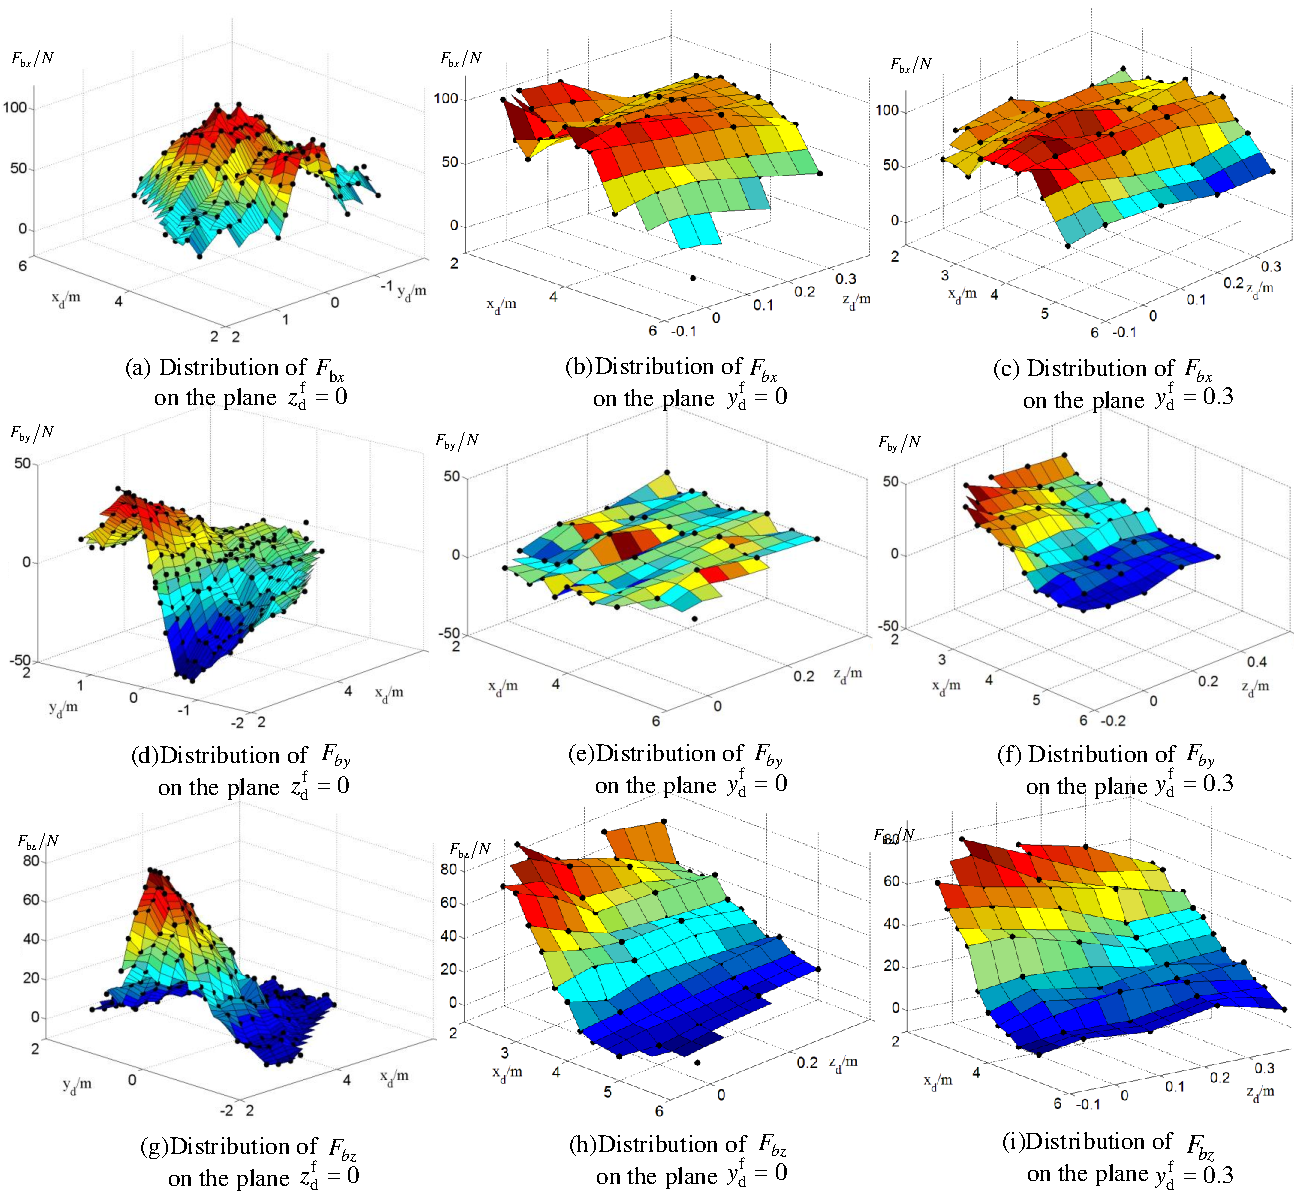
\includegraphics[width=0.7\textwidth]{Figures/Figs_Ch4/fig18.pdf}
	\caption{Distribution of Training Data on Three Main Planes}\label{fig4.15}
\end{figure}
\subsection{Bow Wave Effect Model and Parameter Estimation}

In this section, the form of the function ${{\bf{F}}_{\rm{b}}}\left( { {{\bf{p}}}_{\rm{d}}^{\rm{f}}} \right)$ will be first speculated, then the parameters in the model will be estimated using the training data, and finally the model will be validated using all the training data. If the validation is successful, it confirms the correctness of the speculated function form.

\subsubsection{Speculating the Functional Form of the Bow Wave Effect Model}

(1) Functional Form

First, the speculated form of the function is provided 
\begin{equation}\label{eq4.106}
{ {{\bm{f}}}_{\rm{b}}}\left( { {{\bf{p}}}_{\rm{d}}^{\rm{f}}} \right) = \left[ {\begin{array}{*{20}{c}}
	{{ {{\bm{f}}}_{{\rm{b}}x}}\left( { {{\bf{p}}}_{\rm{d}}^{\rm{f}}} \right)}\\
	{{ {{\bm{f}}}_{{\rm{b}}y}}\left( { {{\bf{p}}}_{\rm{d}}^{\rm{f}}} \right)}\\
	{{ {{\bm{f}}}_{{\rm{b}}z}}\left( { {{\bf{p}}}_{\rm{d}}^{\rm{f}}} \right)}
	\end{array}} \right] = \left[ {\begin{array}{*{20}{c}}
	{{F_{{\rm{b}}x}}}\\
	{{F_{{\rm{b}}y}}}\\
	{{F_{{\rm{b}}z}}}
	\end{array}} \right] = \left[ {\begin{array}{*{20}{c}}
	{{F_{{\rm{b}}x\_{\rm{nose}}}} + {F_{{\rm{b}}x\_cockpit}}}\\
	{{F_{{\rm{b}}y}}}\\
	{{F_{{\rm{b}}z}}}
	\end{array}} \right]
\end{equation}
where 
\begin{equation}\label{eq4.107}
\left\{ \begin{aligned}
&{F_{{\rm{b}}x\_{\rm{nose}}}} = {{\rm{C}}_{x1}}\left[ {1 - {{\rm{C}}_{x2}}{{\left( {x_{\rm{d}}^{\rm{f}} - {{\rm{C}}_{x3}}} \right)}^2}} \right]{e^{\frac{{ - {{\left( {y_{\rm{d}}^{\rm{f}}} \right)}^2}}}{{{{\rm{C}}_{x4}}}}}}{e^{\frac{{z_{\rm{d}}^{\rm{f}}}}{{{{\rm{C}}_{x5}}}}}}s\left( {\frac{1}{{\sqrt {{{\rm{C}}_{x2}}} }} + {{\rm{C}}_{x3}} - x_{\rm{d}}^{\rm{f}}} \right)\\
&{F_{{\rm{b}}x\_{\rm{cockpit}}}} = {{\rm{C}}_{x6}}\left( {1 - {{\rm{C}}_{x7}}x_{\rm{d}}^{\rm{f}}} \right){e^{\frac{{ - {{\left( {y_{\rm{d}}^{\rm{f}}} \right)}^2}}}{{{{\rm{C}}_{x8}}}}}}{e^{\frac{{z_{\rm{d}}^{\rm{f}}}}{{{{\rm{C}}_{x9}}}}}}s\left( {\frac{1}{{{{\rm{C}}_{x7}}}} - x_{\rm{d}}^{\rm{f}}} \right)\\
&{F_{{\rm{b}}y}} = {{\rm{C}}_{y1}}\left( {1 - {{\rm{C}}_{x2}}x_{\rm{d}}^{\rm{f}}} \right)y_{\rm{d}}^{\rm{f}}{e^{\frac{{ - {{\left( {y_{\rm{d}}^{\rm{f}}} \right)}^2}}}{{{{\rm{C}}_{y3}}}}}}{e^{\frac{{z_{\rm{d}}^{\rm{f}}}}{{{{\rm{C}}_{y4}}}}}}s\left( {\frac{1}{{{{\rm{C}}_{y2}}}} - x_{\rm{d}}^{\rm{f}}} \right)\\
&{F_{{\rm{b}}z}} =  - {{\rm{C}}_{z1}}\left( {1 - {{\rm{C}}_{z2}}x_{\rm{d}}^{\rm{f}}} \right){e^{\frac{{ - {{\left( {y_{\rm{d}}^{\rm{f}}} \right)}^2}}}{{{{\rm{C}}_{z3}}}}}}{e^{\frac{{z_{\rm{d}}^{\rm{f}}}}{{{{\rm{C}}_{z4}}}}}}s\left( {\frac{1}{{{{\rm{C}}_{z2}}}} - x_{\rm{d}}^{\rm{f}}} \right)
\end{aligned} \right.
\end{equation}
Here, $C_{(\cdot)}\in\mathbb{R}_{+}$ represents the parameters to be identified in the model, and the function $s\left( \sigma  \right)$ is a step function defined as 
\begin{equation}\label{eq4.108}
s\left( \sigma  \right) = \left\{ {\begin{array}{*{20}{c}}
	{1,}&{\sigma  \ge 0}\\
	{0,}&{\sigma  < 0}
	\end{array}} \right.
\end{equation}
This function also represents the effective range of the bow wave in the ${o_{\rm{f}}}{x_{\rm{f}}}$ direction. When the position of the drogue is farther from $\chi $, the bow wave has no effect, that is, ${ {{\mathbf{F}}}_{\rm{b}}} = {\bf{0}}$. The bow wave only comes into play within the range of $\chi $. It should be noted that ${F_{{\rm{b}}x}}$ is decomposed into two parts: one part is caused by the aircraft nose, denoted as ${F_{{\rm{b}}x\_{\rm{nose}}}}$, and the other part is caused by the receiver aircraft fuselage, denoted as ${F_{{\rm{b}}x\_{\rm{cockpit}}}}$. We will explain why this is done in the subsequent sections.

(2) Process of Speculating Functional Form

Taking ${ {{\bm{f}}}_{{\rm{b}}z}}\left( { {{\bf{p}}}_{\rm{d}}^{\rm{f}}} \right)$ as an example, let's explain the process of inferring the functional form. The process of inferring other functions is similar. Fig. \ref{fig4.16} illustrates the three profiles of ${F_{{\rm{b}}z}}$, which are derived from Fig. \ref{fig4.15} (g) and (h). (Note that the training data in Fig. \ref{fig4.16} has been processed, so the direction is opposite to that in Fig. \ref{fig4.15}.)

Step one: Estimate the three functional relationships ${h_{z - x}}\left( {{x_{\rm{d}}}} \right), {h_{z - y}}\left( {{y_{\rm{d}}}} \right)$ and ${h_{z - z}}\left( {{z_{\rm{d}}}} \right)$ based on these three profile plots. (Note that the issue of sign will be considered in the second step.)

1) The curve in Fig. \ref{fig4.16} (a) is nearly linear in the first half, and due to the fact that the bow wave cannot affect the drogue when it is far from the aircraft nose, the second half of the curve must be zero. Therefore, this curve can be expressed by the following equation.
\begin{equation}\label{eq4.109}
{h_{z - x}}\left( {x_{\rm{d}}^{\rm{f}}} \right) = \left( {1 - {{\rm{C}}_{z2}}x_{\rm{d}}^{\rm{f}}} \right) \cdot s\left( {\frac{1}{{{{\rm{C}}_{z2}}}} - x_{\rm{d}}^{\rm{f}}} \right)
\end{equation}
\begin{figure}[th]
	\centering
	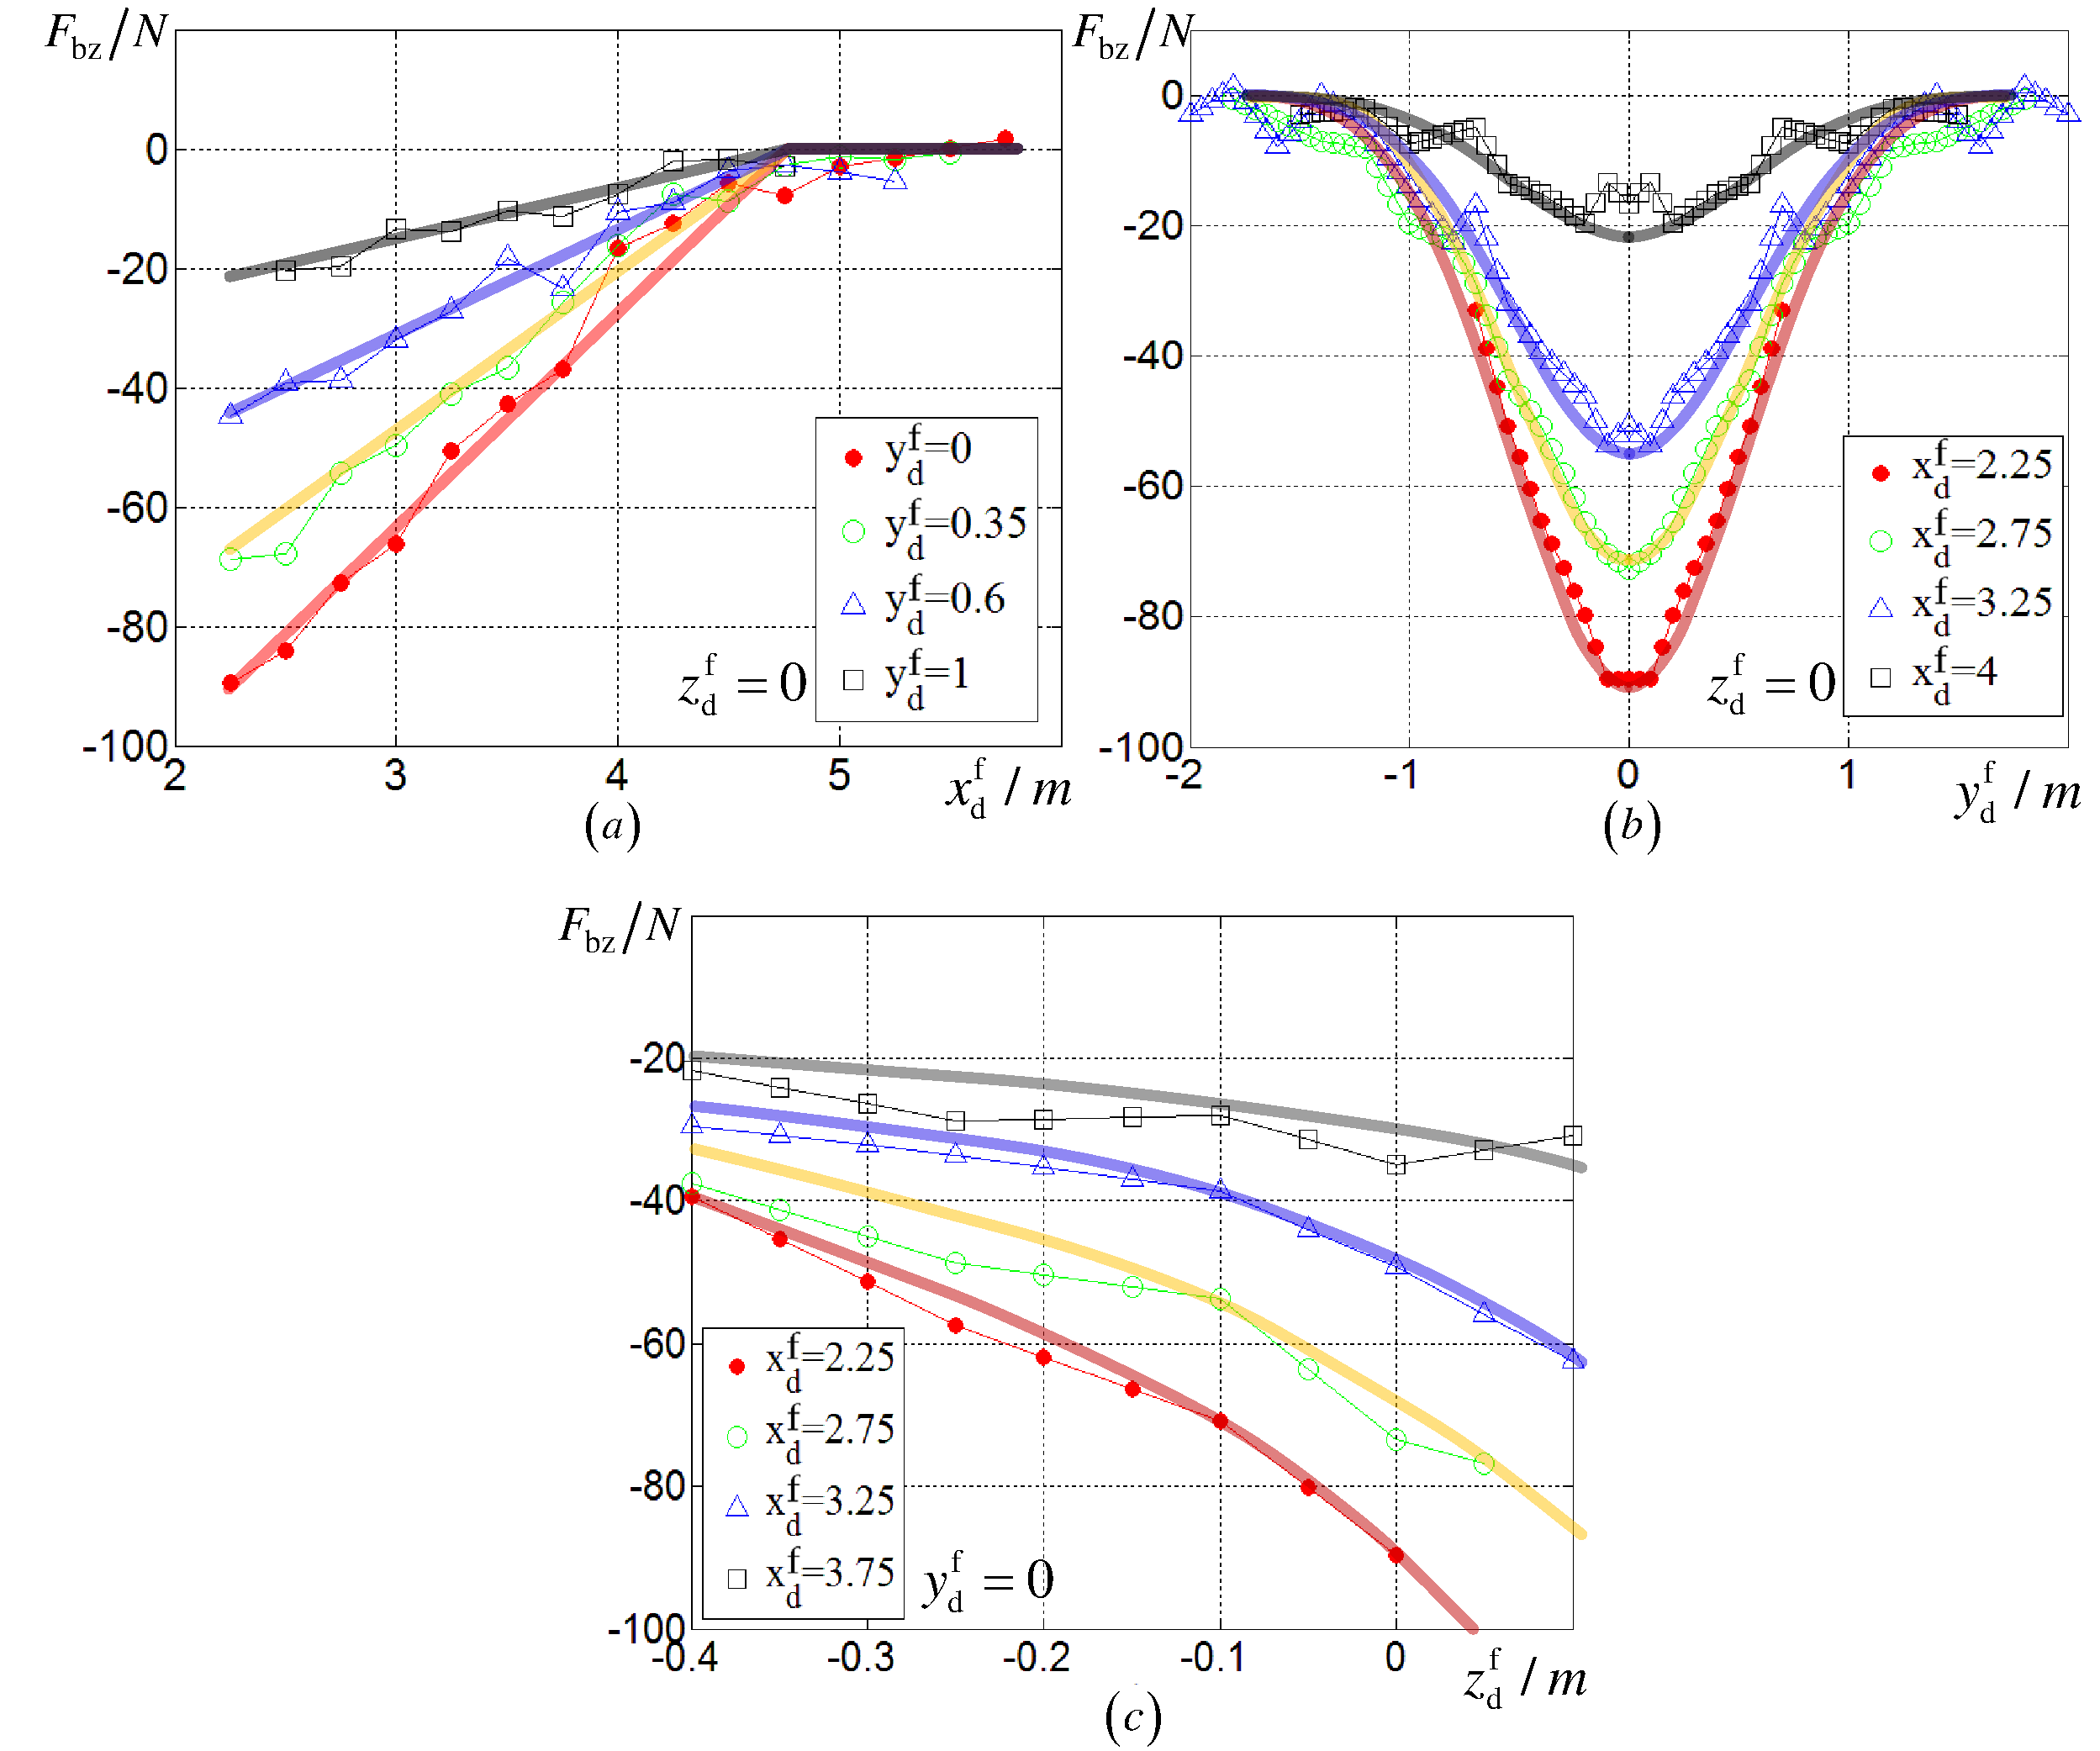
\includegraphics[width=0.7\textwidth]{Figures/Figs_Ch4/fig19.pdf}
	\caption{Distribution of Training Data on Three Main Planes}\label{fig4.16}
\end{figure}
2) The curve in Fig. \ref{fig4.16} (b) approximates a normal distribution curve, thus it can be expressed using the following equation
\begin{equation}\label{eq4.110}
{h_{z - y}}\left( {y_{\rm{d}}^{\rm{f}}} \right) = {e^{\frac{{ - {{\left( {y_{\rm{d}}^{\rm{f}}} \right)}^2}}}{{{{\rm{C}}_{z3}}}}}}
\end{equation}

3) The curve in Fig. \ref{fig4.16} (c) increases in velocity as it progresses, hence it can be expressed using an exponential function.
\begin{equation}\label{eq4.111}
{h_{z - z}}\left( {z_{\rm{d}}^{\rm{f}}} \right) = {e^{\frac{{z_{\rm{d}}^{\rm{f}}}}{{{{\rm{C}}_{z4}}}}}}
\end{equation}

Step two: Assuming the coupling relationships between different directions are 
\begin{equation}\label{eq4.112}
{ {{\bm{f}}}_{{\rm{b}}z}}\left( {\bf {p}_{\rm{d}}^{\rm{f}}} \right) =  - {{\rm{C}}_{z1}}{h_{z - x}}\left( {x_{\rm{d}}^{\rm{f}}} \right){h_{z - y}}\left( {y_{\rm{d}}^{\rm{f}}} \right){h_{z - z}}\left( {z_{\rm{d}}^{\rm{f}}} \right)
\end{equation}
where ${{\rm{C}}_{z1}}$ represents the gain in the function, and due to the fact that ${{\bm{f}}_{{\rm{b}}z}}$ is always positive when in the docking region, there is a negative sign.

The estimation method for ${ {{\bm{f}}}_{{\rm{bx}}}}\left( { {{\bf{p}}}_{\rm{d}}^{\rm{f}}} \right)$ and ${ {{\bm{f}}}_{{\rm{b}}y}}\left( { {{\bf{p}}}_{\rm{d}}^{\rm{f}}} \right)$ is similar to that for ${ {{\bm{f}}}_{{\rm{b}}z}}\left( { {{\bf{p}}}_{\rm{d}}^{\rm{f}}} \right)$, but ${ {{\bm{f}}}_{{\rm{bx}}}}\left( { {{\bf{p}}}_{\rm{d}}^{\rm{f}}} \right)$ is more specific. The following provides the special treatment for it.

(3) Special Treatment of ${ {{\bm{f}}}_{{\rm{b}}x}}\left( { {{\bf{p}}}_{\rm{d}}^{\rm{f}}} \right)$

Fig. \ref{fig4.17} shows the cross-sectional profile of ${F_{{\rm{b}}x}}$ within the $z_{\rm{d}}^{\rm{f}} = 0$ plane. During the subsequent parameter fitting process, it is found that using a single function to express ${h_{x - x}}\left( {x_{\rm{d}}^{\rm{f}}} \right)$ alone cannot pass the goodness-of-fit test based on the determination coefficient (see Section 4.3.3.3). Therefore, according to Fig. \ref{fig4.17}, separating the two components that influence ${f_{{\rm{b}}x}}$ and fitting them separately yields a well-fitted result. These two components are a parabola and a straight line, and further analysis reveals that they correspond to two distinct parts of the bow wave: the bow wave from the aircraft nose and the bow wave from the cockpit.

\subsubsection{Parameter Estimation of the Model}

Estimating the parameters in Eq. (\ref{eq4.107}) using the training data is the next step. Similarly, take ${ {{\bm{f}}}_{{\rm{b}}z}}\left( { {{\bf{p}}}_{\rm{d}}^{\rm{f}}} \right)$ as an example. Since it involves parameters, it can be rewritten as ${ {{\bm{f}}}_{{\rm{b}}z}}\left( { {{\bf{p}}}_{\rm{d}}^{\rm{f}},{\mathbf{C}_z}} \right)$, where ${\mathbf {C}_z} = {\left[ {\begin{array}{*{20}{c}}
		{{{\rm{C}}_{z1}}}&{{{\rm{C}}_{z2}}}&{{{\rm{C}}_{z3}}}&{{{\rm{C}}_{z4}}}
		\end{array}} \right]^{\rm{T}}}\in\mathbb{R}^{4}_{+}$ represents the unknown parameters. Accordingly, the corresponding optimization problem can be expressed as 
\begin{equation}\label{eq4.113}
\mathbf {C}_z^* = \mathop {\arg \min }\limits_{{\mathbf {C}_z} \in \mathbb{R}^{4}_{+}} \sum\limits_{i = 1}^{{N_{\rm{f}}}} {{{\left[ {{F_{{\rm{b}}z,i}} - { {{\bm{f}}}_{{\rm{b}}z}}\left( { {{\bf{p}}}_{{\rm{d}},i}^{\rm{f}},{\mathbf {C}_z}} \right)} \right]}^2}} 
\end{equation}
where ${N_{\rm{f}}}$ represents the number of training data points used for parameter estimation. For the initial value selection of this optimization, one can perform a single function fitting on the curves within the profiles and use the obtained parameters as initial values. For example, when estimating ${ {{\bm{f}}}_{{\rm{b}}z}}\left( { {{\bf{p}}}_{\rm{d}}^{\rm{f}},{\mathbf {C}_z}} \right)$, one can choose the initial value as ${\mathbf {C}_{z0}} = {\left[ {\begin{array}{*{20}{c}}
		{170}&{0.2}&{0.5}&{0.6}
		\end{array}} \right]^{\rm{T}}}$.
\begin{figure}[th]
	\centering
	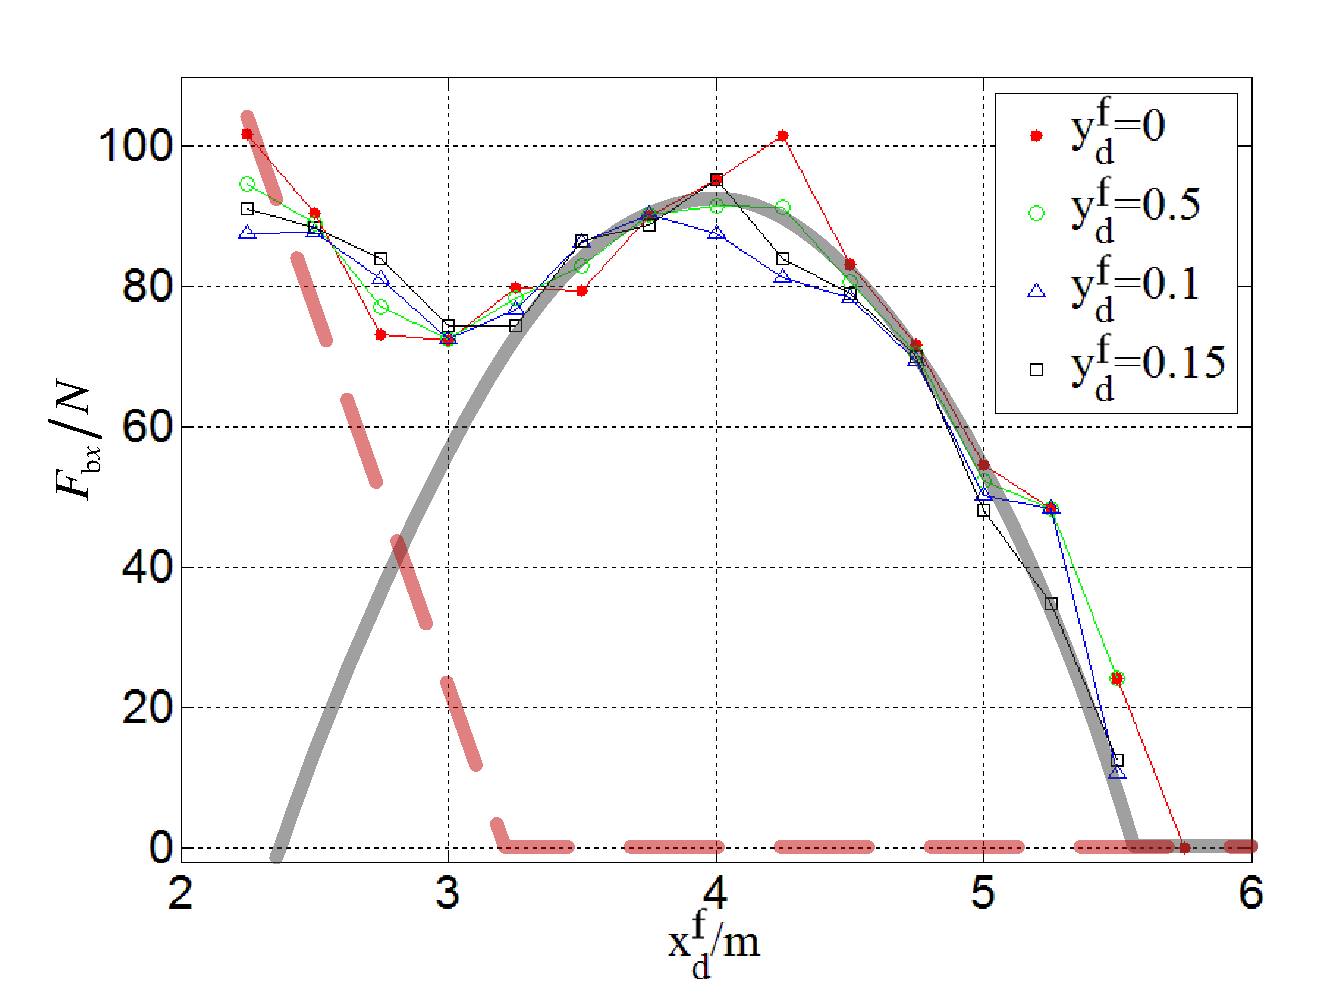
\includegraphics[width=0.7\textwidth]{Figures/Figs_Ch4/fig20.pdf}
	\caption{Two Components Constituting ${F}_{\rm{b}x}$}\label{fig4.17}
\end{figure}
After setting the initial values, one can use the nonlinear fitting function nlinfit provided by MATLAB® to obtain $\mathbf {C}_z^*$. The estimation method for $\mathbf {C}_y^*$ in ${ {{\bm{f}}}_{{\rm{b}}y}}\left( { {{\bf{p}}}_{\rm{d}}^{\rm{f}},{\mathbf {C}_y}} \right)$ is the same as for $ \mathbf{C}_z^*$. As for ${ {{\bm{f}}}_{{\rm{b}}x}}\left( { {{\bf{p}}}_{\rm{d}}^{\rm{f}},{\mathbf {C}_x}} \right)$, the contribution from the nose section can be first estimated. Then, subtract the estimated nose contribution from the training data to obtain new training data, and estimate the cockpit contribution from this data.
By substituting the estimated values of $\mathbf {C}_x^*, \mathbf{C}_y^*$ and $\mathbf{C}_z^*$ into Eq. (\ref{eq4.107}), the bow wave effect model can be obtained under these conditions as follows 
\begin{equation}\label{eq4.114}
\left\{ \begin{aligned}
&{F_{{\rm{b}}x\_{\rm{nose}}}} = 91.6170\left[ {1 - 0.3220{{\left( {x_{\rm{d}}^{\rm{f}} - 3.8870} \right)}^2}} \right]{e^{\frac{{ - {{\left( {y_{\rm{d}}^{\rm{f}}} \right)}^2}}}{{2.7395}}}}{e^{\frac{{z_{\rm{d}}^{\rm{f}}}}{{2.4838}}}}s\left( {5.6493 - x_{\rm{d}}^{\rm{f}}} \right)\\
&{F_{{\rm{b}}x\_{\rm{cockpit}}}} = 309.7709\left( {1 - 0.3237x_{\rm{d}}^{\rm{f}}} \right){e^{\frac{{ - {{\left( {y_{\rm{d}}^{\rm{f}}} \right)}^2}}}{{0.3851}}}}{e^{\frac{{z_{\rm{d}}^{\rm{f}}}}{{1.1471}}}}s\left( {3.0893 - x_{\rm{d}}^{\rm{f}}} \right)\\
&{F_{{\rm{b}}y}} = 223.3210\left( {1 - 0.2082x_{\rm{d}}^{\rm{f}}} \right)y_{\rm{d}}^{\rm{f}}{e^{\frac{{ - {{\left( {y_{\rm{d}}^{\rm{f}}} \right)}^2}}}{{0.8102}}}}{e^{\frac{{z_{\rm{d}}^{\rm{f}}}}{{0.6555}}}}s\left( {4.8031 - x_{\rm{d}}^{\rm{f}}} \right)\\
&{F_{{\rm{b}}z}} =  - 173.2021\left( {1 - 0.2141x_{\rm{d}}^{\rm{f}}} \right){e^{\frac{{ - {{\left( {y_{\rm{d}}^{\rm{f}}} \right)}^2}}}{{0.5697}}}}{e^{\frac{{z_{\rm{d}}^{\rm{f}}}}{{0.7038}}}}s\left( {4.6707 - x_{\rm{d}}^{\rm{f}}} \right)
\end{aligned} \right.
\end{equation}

\subsubsection{Validating the Effectiveness of the Parameters}

To validate the effectiveness of the parameters, the coefficient of determination \cite{weisberg_applied_2005} is chosen as the criterion for evaluating the fitting performance, denoted as ${{{\cal R}}^2}$. Taking ${ {{\bm{f}}}_{{\rm{b}}z}}\left( { {{\bf{p}}}_{\rm{d}}^{\rm{f}},{\mathbf {C}_z}} \right)$ as an example, its corresponding coefficient of determination is defined as 
\begin{equation}\label{eq4.115}
{{\cal R}}_z^2 = 1 - \frac{{{\rm{SS}}{{\rm{E}}_z}}}{{{\rm{SS}}{{\rm{T}}_z}}}
\end{equation}
where 
\begin{equation}\label{eq4.116}
\left\{ \begin{aligned}
&{\rm{SS}}{{\rm{E}}_z} = \sum\limits_{i = 1}^{{N_{\rm{v}}}} {{{\left[ {{f_{{\rm{b}}z,i}} - {F_{{\rm{b}}z}}\left( { {{\bm{p}}}_{{\rm{d}},i}^{\rm{f}},\bm {C}_z^*} \right)} \right]}^2}} \\
&{\rm{SS}}{{\rm{T}}_z} = \sum\limits_{i = 1}^{{N_{\rm{v}}}} {{{\left[ {{f_{{\rm{b}}z,i}} - \frac{1}{{{N_{\rm{f}}}}}\sum\limits_{i = 1}^{{N_{\rm{v}}}} {{f_{{\rm{b}}z,i}}} } \right]}^2}} 
\end{aligned} \right.
\end{equation}
where ${N_{\rm{v}}}$ is the number of training points used for validation. According to this definition, it can derived 
\begin{equation}\label{eq4.117}
{{\cal R}}_x^2 = 0.8866,{{\cal R}}_y^2 = 0.9536,{{\cal R}}_z^2 = 0.9671
\end{equation}
Generally speaking, when ${{{\cal R}}^2} > 0.7$, the fitting results are considered good. Therefore, based on Eq. (\ref{eq4.117}), it can be concluded that the speculated model and the estimated parameters are consistent with the bow wave effect.

Fig. \ref{fig4.18} presents the comparison between the surface formed by ${ {{\bm{f}}}_{{\rm{b}}z}}\left( { {{\bf{p}}}_{\rm{d}}^{\rm{f}}, \mathbf{C}_z^*} \right)$ on the plane $z_{\rm{d}}^{\rm{f}} = 0$ and the training data of ${F_{{\rm{b}}x}}$ (represented by the black dots in the figure), corresponding to Fig. \ref{fig4.15}(a). The function ${{\bm{f}}}_{{\rm{b}}z}$ is one of the more complex functions in the bow wave effect model, and Fig. \ref{fig4.18} intuitively demonstrates how well ${ {{\bm{f}}}_{{\rm{b}}z}}\left( { {{\bf{p}}}_{\rm{d}}^{\rm{f}}, \mathbf {C}_z^*} \right)$ captures the trend of ${F_{{\rm{b}}x}}$ changing with the relative position of the drogue and the receiver aircraft.
\begin{figure}[th]
	\centering
	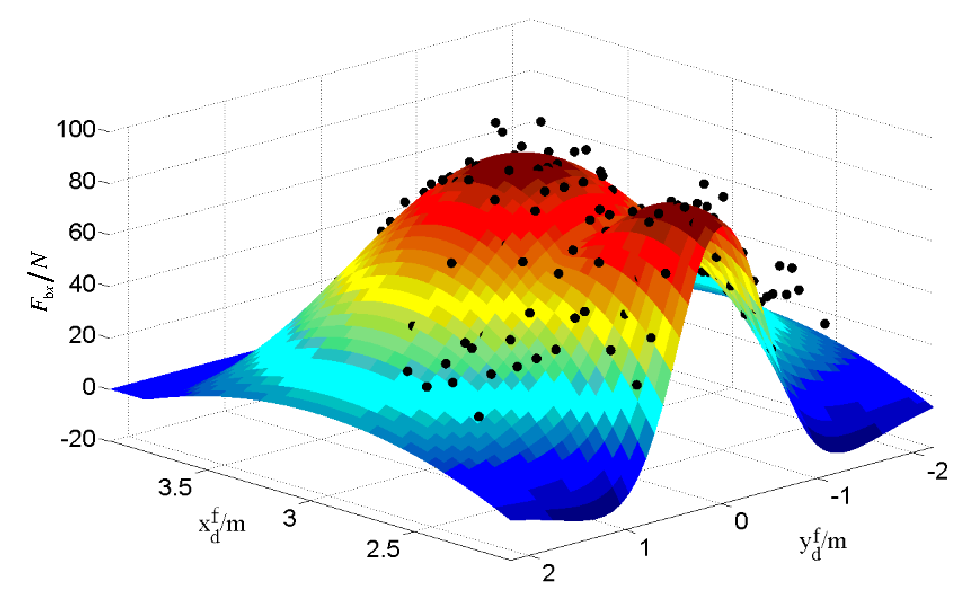
\includegraphics[width=0.7\textwidth]{Figures/Figs_Ch4/fig21.pdf}
	\caption{Fitting Effect of $\bm{F}_{\rm{b}x}$}\label{fig4.18}
\end{figure}
\subsubsection{Matters Needing Attention for Applying the Bow Wave Effect Model}

The modeling method for the bow wave effect described in this chapter, while providing an example model for a specific environment (as shown in Table \ref{tab4.2}) and a specific aircraft type, can be extended to model bow wave effects for different aircraft types in various environments. However, when applying this method or model, it's important to consider its application conditions and scope.

(1) Application Conditions: The model (\ref{eq4.107}) is developed based on aircraft with an ellipsoidal cone nose, making this function form suitable for such aircraft types as F-16, F-18, J-8, and similar ones. For aircraft with non-ellipsoidal cone nose, the modeling process remains applicable, but the function form would need to be adjusted compared with Eq. (\ref{eq4.106}). For instance, aircraft like the X-47B, which has already undergone autonomous docking experiments and features a flying-wing design, can be considered to have a two-dimensional nose rather than a three-dimensional one, leading to a relatively simpler model. Another scenario involves aircraft with canard wings, like the J-10; if the canards are mounted toward the front, they would also need to be included in the modeling process.

(2) Application Scope: The data used to establish this model is obtained from the ${{\bf{p}}}_{{\rm{d}},i}^{\rm{f}} \in \left[ {2,6} \right] \times \left[ { - 2,2} \right] \times \left[ { - 0.5,0.1} \right]$ region. As a result, the model is more accurate within this specific area. Nevertheless, the model remains applicable in the surrounding areas of this region. Furthermore, considering that ${ \bf{F}_{\rm{b}}} = {\bf{0}}$ when $x_{\rm{d}}^{\rm{f}} > 6$ due to the bow wave not affecting the drogue, it is evident that model (\ref{eq4.106}) fulfills this condition. Consequently, the model (\ref{eq4.106}) is equally applicable within the region where $x_{\rm{d}}^{\rm{f}} > 6$.

Additionally, there are two points that require clarification:

(1) When modeling the force ${F_{{\rm{b}}x}}$, the force was divided into two components: the forces from the nose and the cockpit. However, when modeling ${F_{{\rm{b}}y}}$ and ${F_{{\rm{b}}z}}$, the cockpit was not taken into consideration. The reason for this lies in Eq. (\ref{eq4.113}), which indicates that the range of force in the ${F_{{\rm{b}}x}}$ direction is relatively extensive. Referring to the parameters in Figure 4.11, it can be observed that ${F_{{\rm{b}}x\_{\rm{nose}}}}$ becomes effective at approximately 1.2 meters in front of the nose, whereas the effective range of ${F_{{\rm{b}}y}}$ and ${F_{{\rm{b}}z}}$ is only about 0.5 meters in front of the nose. This situation implies that, before the probe docks with the drogue, the force component ${F_{{\rm{b}}x\_{\rm{cockpit}}}}$ from the cockpit has an effect, while the cockpit hasn't yet influenced the other two directions. Therefore, it was not included in the modeling. However, if the position of the probe continues to shift backward, this component will also need to be included in the modeling. This is also why aircraft with canard wings need to be accounted for in the model.

(2) The use of a linear expression for the portion related to $x_{\rm{d}}^{\rm{f}}$ in the model is due to the relatively good linearity of this part within the docking region. However, in reality, if viewed over a larger range, this part is not necessarily linear. For example, the effect of ${F_{{\rm{b}}x\_{\rm{nose}}}}$ caused by the nose section with respect to $x_{\rm{d}}^{\rm{f}}$ follows a quadratic curve. Therefore, the choice of function form is closely related to the range considered.

\subsection{Simulation Analysis and Model Validation of the Bow Wave Effect}

By incorporating the bow wave effect model into the link-connected hose-drogue model, the motion trajectory of the drogue under the influence of the bow wave effect can be derived. By comparing this with the publicly available experimental data from NASA \cite{dibley_autonomous_2007}, we can further validate the effectiveness of the model. Additionally, this allows to analyze the motion of the drogue during the docking process.

\subsubsection{Setting of Simulation Environment and Simulation Results}

The bow wave effect model and the link-connected hose-drogue model (without HDU and with fixed-length hose) are integrated into the same simulation, as depicted in Fig. \ref{fig4.19}. In order to closely replicate experimental conditions, white noise and a low-pass filter are introduced to simulate the impact of atmospheric turbulence on the drogue. A total of six sets of experimental data are provided in Ref. \cite{dibley_autonomous_2007}. Among them, the sixth set of experiments had relatively stable airflow, making it suitable for observing the bow wave effect. Hence, this set of experiments is selected  as the control group. Since the experiments in the reference used the drogue equilibrium point coordinate system, we also transformed all the data into the drogue equilibrium point coordinate system.
\begin{figure}[th]
	\centering
	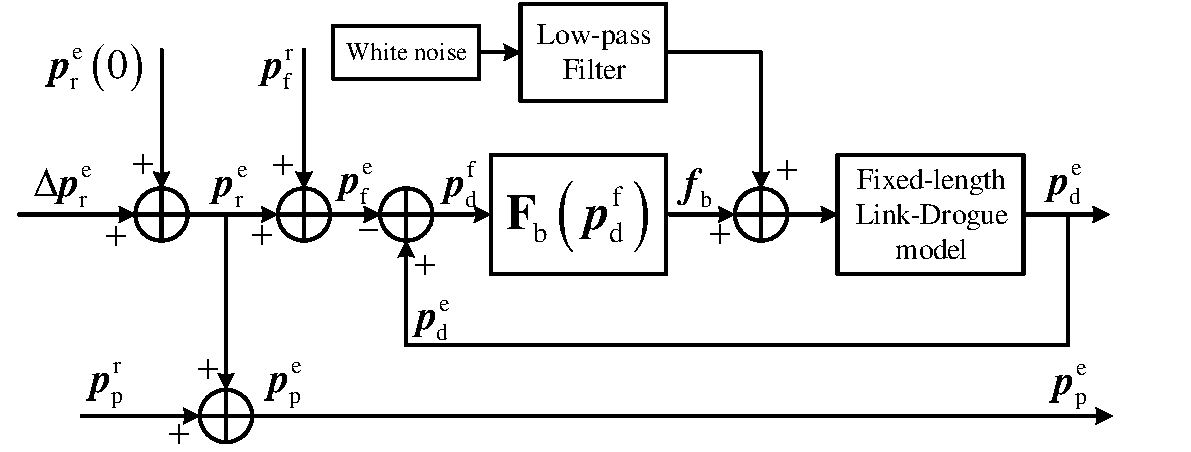
\includegraphics[width=0.7\textwidth]{Figures/Figs_Ch4/fig22.pdf}
	\caption{Schematic Diagram of Drogue Dynamics Simulation under Bow Wave Effect}\label{fig4.19}
\end{figure}

Ref. \cite{dibley_autonomous_2007} does not provide the docking environment parameters or specific docking controller details. Therefore, we still assume the environment to be the same as in Table \ref{tab4.2}. The specific parameters of the receiver aircraft are as shown in Fig. \ref{fig4.11}. In the absence of a docking controller, we assume the receiver aircraft flies at a constant speed. Although this approach may introduce some deviations, it is sufficient for qualitative analysis of the drogue's dynamics. To ensure that the receiver aircraft's trajectory is closer to the trajectory of Experiment 6 in Ref. \cite{dibley_autonomous_2007}, we set its initial position as $ {{\bf{p}}}_{\rm{r}}^{\rm{e}}\left( 0 \right) = {\left[ {\begin{array}{*{20}{c}}
		{ - 12}&{ - 0.54}&{0.86}
		\end{array}} \right]^{\rm{T}}}$ and its trajectory as $\Delta  {{\bf{p}}}_{\rm{r}}^{\rm{e}} = {\left[ {\begin{array}{*{20}{c}}
		{\Delta x_{\rm{r}}^{\rm{e}}}&0&0
		\end{array}} \right]^{\rm{T}}}$, where $\Delta x_{\rm{r}}^{\rm{e}}$ satisfies the following equation 
\begin{equation}\label{eq4.118}
{\left[ {\Delta x_{\rm{r}}^{\rm{e}}\left( t \right)} \right]^{\prime \prime \prime }}{\rm{ = }}\left\{ {\begin{array}{*{20}{l}}
	{0,}&{t = 0 \cup t \in \left( {16, + \infty } \right)}\\
	{0.047,}&{t \in \left( {0,4} \right] \cup t \in \left( {12,16} \right]}\\
	{ - 0.047,}&{t \in \left( {4,12} \right]}
	\end{array}} \right.,{\rm{    }}\Delta x_{\rm{r}}^{\rm{e}}\left( 0 \right) = 0
\end{equation}
Under the influence of $\Delta  {{\bf{p}}}_{\rm{r}}^{\rm{e}}$, the motion trajectory of the drogue and the probe can be seen in Fig. \ref{fig4.20}. In this figure, figures (a), (c), and (e) show the original data from Experiment 6 in Ref. \cite{dibley_autonomous_2007}, while figures. (b), (d), and (f) display the simulation results. "Longitudinal" corresponds to the ${o_{\rm{e}}}{x_{\rm{e}}}$ direction, "Lateral" to the ${o_{\rm{e}}}{y_{\rm{e}}}$ direction, and "Vertical" to the $ - {o_{\rm{e}}}{z_{\rm{e}}}$ direction (in the experiment, upward is positive, so it is opposite to the ${o_{\rm{e}}}{z_{\rm{e}}}$ direction).

The symbol ${{\rm{X}}_{{\rm{MISS}}}}$ represents the position where the probe contacts the plane of the drogue's parachute in the ${o_{\rm{e}}}{x_{\rm{e}}}$ direction, and ${{\rm{X}}_{{\rm{CAP}}}}$ is the position where the probe and the drogue are connected to complete the docking. It's worth noting that due to the use of the imperial system in the experiment, the length units in this figure have all been converted to feet.
To provide a more intuitive view of this process, we utilized the Virtual Reality toolbox provided by MATLAB® to record a video of this process (as shown in Fig. \ref{fig4.21}). This video can be viewed in Ref. \cite{noauthor_drogue_nodate}. In the video, Viewpoint 1 represents the pilot's perspective, Viewpoint 2 provides a side view, Viewpoint 3 offers the tanker's perspective, and Viewpoint 4 demonstrates the relationship between the drogue and the probe in the vertical plane.

\subsubsection{Simulation Analysis and Model Validation}

(1) Dynamic Analysis of Drogue under Bow Wave Effect

From the simulation results, the dynamic behavior of the drogue under the influence of the bow wave during the docking process can be summarized as follows:

1) As shown in Fig. \ref{fig4.20}, during the time interval from 0s to 8s, the aircraft's nose is far from the drogue, so the drogue is not affected by the bow wave effect.

2) As depicted in Figs. \ref{fig4.20} (e) and (f), from 8s to 10s, the aircraft's nose begins to approach the drogue, and due to the influence of $\bm{f}_{\rm{bx\_nose}}$, the drogue starts to descend.

3) As shown in Figs. \ref{fig4.20} (c), (d), (e), and (f), from 10s to ${t_{{{\rm{X}}_{{\rm{MISS}}}}}}$, the aircraft's nose surpasses the drogue, causing the drogue to swing upwards and to the right. Here, ${t_{{{\rm{X}}_{{\rm{MISS}}}}}}$ represents the moment when the aircraft's nose reaches ${{{\rm{X}}_{{\rm{MISS}}}}}$.

4) Based on the simulation results, the motion of the drogue appears to exhibit characteristics similar to those of a second-order dynamic system. Thus, it can be observed from the simulation that if the drogue were to move freely, its trajectory in the final stage would resemble a three-dimensional spiral. In other words, if the docking is not successful, the drogue would swing back. During this time, if the receiver does not retract promptly, the drogue is likely to collide with the probe.

Please note that these descriptions are based on the simulation results and provide insights into the potential behavior of the drogue under the influence of the bow wave effect during the docking process.

(2) Comparison Analysis between Simulation and Experiment

From the dashed ellipses in Fig. \ref{fig4.20}, it can be observed that despite the differences in conditions between simulation and experiment, the overall trend of the drogue's dynamics in the simulation closely matches the experimental data. This further validates the effectiveness of the bow wave effect model. However, there are still some differences between the simulation and experimental trajectories, which can be analyzed based on the discrepancies between the two.

1) In the experiment, the encounter between the drogue and the probe has already occurred at ${t_{{{\rm{X}}_{{\rm{MISS}}}}}}$, and the drogue's subsequent data lacks meaning.

2) Due to the absence of docking controllers in the provided literature [12], the simulation does not include such a controller. Consequently, the simulated probe does not actively approach the drogue.

3) There is a time drift between the simulation and experiment. This is because in the experiment, the probe approaches the drogue earlier at ${t_{{{\rm{X}}_{{\rm{MISS}}}}}}$, as shown in Figs. \ref{fig4.20} (a) and (b), which causes a drift in Figs. \ref{fig4.20} (c), (d), (e), and (f).

4) As indicated by the boxed lines in Figs. \ref{fig4.20} (c) and (d), the simulated drogue rises and then falls in the ${o_{\rm{e}}}{y_{\rm{e}}}$ direction, whereas this descent phenomenon does not occur in the experiment. This is due to the presence of docking controllers in the experiment, which causes the receiver to approach the drogue and increase ${F_{{\rm{b}}y}}$, preventing the drogue from descending. Since the simulation lacks docking controllers, this phenomenon is absent.

5) As shown within the circles in Figs. \ref{fig4.20} (e) and (f), the simulated drogue's descent is significantly greater than that observed in the experiment. This phenomenon occurs around $8s$ to $10s$, when only ${F_{{\rm{b}}x\_{\rm{nose}}}}$ is active. This discrepancy suggests that the drogue experienced an ${o_{\rm{e}}}{z_{\rm{e}}}$ displacement when subjected to the ${o_{\rm{e}}}{x_{\rm{e}}}$ direction force in the simulation, possibly due to inadequate consideration of drogue dynamics.

In summary, the first four differences are primarily due to variations in the simulation environment and the presence of docking controllers, unrelated to the model established. However, the last point results from insufficient consideration of the drogue's dynamics. This is mainly because the link-connected hose-drogue model employed here does not consider the dynamic effects of the Hose Drum Unit (HDU). Thus, in the next section, we will discuss the impact of the HDU on the drogue's dynamics during the docking process and simplify the complex link-connected hose-drogue model.
\begin{figure}[htbp]
	\centering
	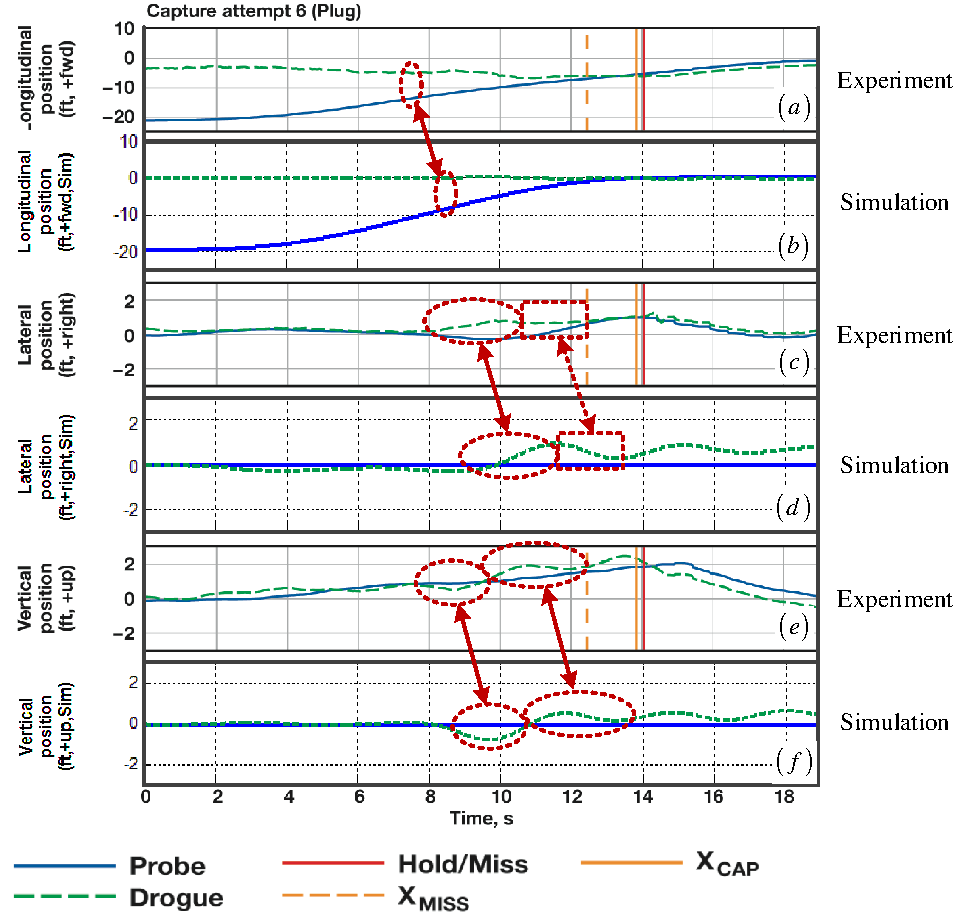
\includegraphics[width=0.7\textwidth]{Figures/Figs_Ch4/fig23.pdf}
	\caption{Comparison of Simulation Data with Experiments in Ref. \cite{dibley_autonomous_2007}}\label{fig4.20}
\end{figure}
\begin{figure}[htbp]
	\centering
	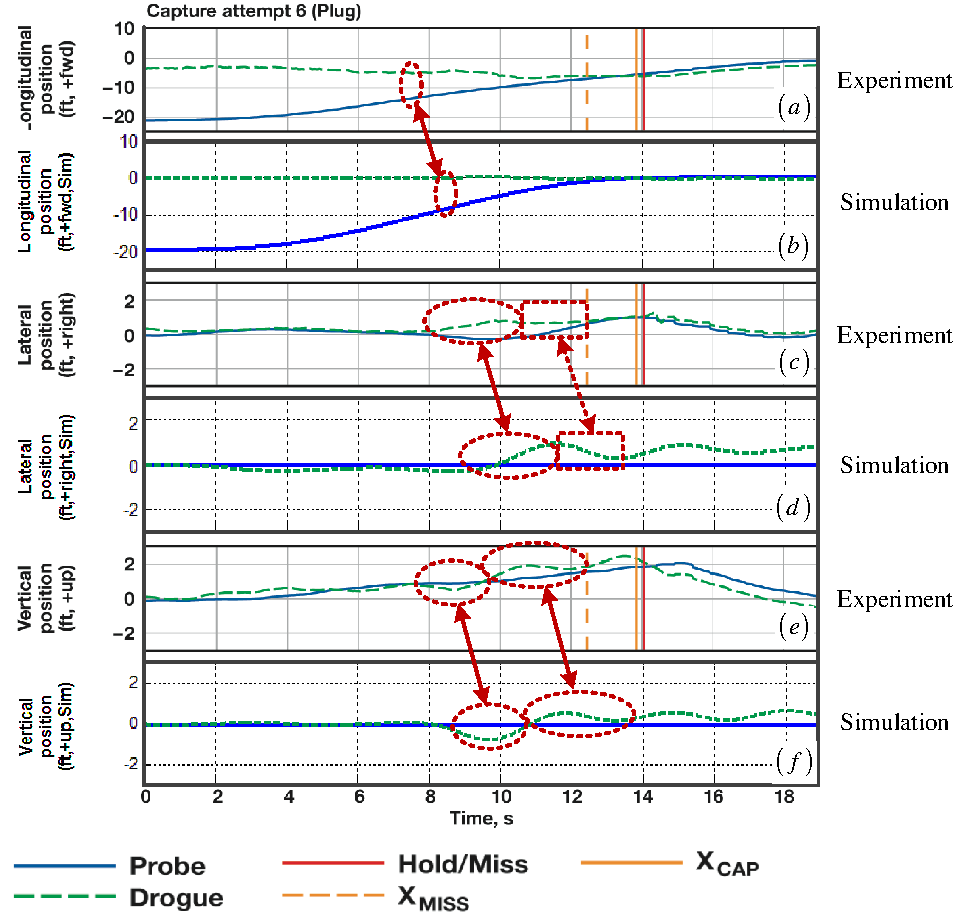
\includegraphics[width=0.7\textwidth]{Figures/Figs_Ch4/fig23.pdf}
	\caption{Screenshots from Simulation Videos}\label{fig4.21}
\end{figure}
\subsection{Appendix: Training Data for CFD Simulation}

% Table generated by Excel2LaTeX from sheet 'Sheet1'
\begin{longtable}{|c|c|c|c|c|c|}
	%	\centering
	\caption{Training Data for CFD Simulation}
	% ?????	 
	\\	\hline	$x_{\rm{d}}^{\rm{f}}$ & $y_{\rm{d}}^{\rm{f}}$  & $z_{\rm{d}}^{\rm{f}}$  &  ${f_{{\rm{b}}x{\rm{o}}}}$  &  ${f_{{\rm{by}}}}$ & $ - {f_{{\rm{bz}}}}$  \\ \hline
	\endfirsthead
	
	
	\multicolumn{6}{c}%
	{{\bfseries \tablename\ \thetable{} -- continued from previous page}} \\	
	\hline	$x_{\rm{d}}^{\rm{f}}$&$y_{\rm{d}}^{\rm{f}}$       & $z_{\rm{d}}^{\rm{f}}$    &  ${f_{{\rm{b}}x{\rm{o}}}}$     &  ${f_{{\rm{by}}}}$    &$ - {f_{{\rm{bz}}}}$  \\ \hline
	% ??????????????????????????????????????	
	\endhead	
	
	
	\hline \multicolumn{6}{r}{{Continued on next page}} \\ \hline
	\endfoot
	
	\hline \hline
	\endlastfoot	
	
	2     & 0.4   & 0     & 1935.152 & 49.97507 & 67.78349 \\ 
	2     & 0.55  & 0     & 1962.551 & 49.90587 & 56.38194 \\ 
	2     & 0.7   & 0     & 1965.541 & 53.56217 & 42.26877 \\	
	2.25  & 0     & 0     & 1877.09 & -1.38444 & 89.50524 \\	
	2.25  & 0.1   & 0     & 1891.363 & 8.478858 & 89.55186 \\	
	2.25  & 0.2   & 0     & 1884.143 & 23.14848 & 79.688 \\ 	
	2.25  & 0.4   & 0     & 1907.8 & 42.64901 & 65.19876 \\	
	2.25  & 0.55  & 0     & 1931.28 & 43.14221 & 50.70876 \\	
	2.25  & 0.7   & 0     & 1948.082 & 44.39585 & 32.93854 \\	
	2.5   & 0     & 0     & 1888.471 & -3.3283 & 84.03368 \\	
	2.5   & 0.1   & 0     & 1891.097 & 12.75222 & 78.3916 \\ 
	2.5   & 0.2   & 0     & 1889.646 & 17.89514 & 77.71612 \\ 
	2.5   & 0.3   & 0     & 1891.902 & 29.18447 & 70.80311 \\
	2.5   & 0.4   & 0     & 1912.455 & 38.22988 & 64.80012 \\
	2.5   & 0.55  & 0     & 1925.106 & 37.56345 & 41.95024 \\
	2.5   & 0.7   & 0     & 1937.53 & 40.44554 & 33.88661 \\
	2.75  & 0     & 0     & 1905.588 & -1.54709 & 72.78587 \\
	2.75  & 0.1   & 0     & 1897.696 & 10.06669 & 70.35958 \\
	2.75  & 0.2   & 0     & 1891.794 & 14.38844 & 65.44239 \\
	2.75  & 0.4   & 0     & 1916.689 & 29.95287 & 50.69795 \\
	2.75  & 0.55  & 0     & 1908.102 & 29.90309 & 43.66149 \\
	2.75  & 0.7   & 0     & 1925.605 & 34.67043 & 28.83245 \\
	2.75  & 0.8   & 0     & 1927.103 & 30.74913 & 22.5957 \\
	2.75  & 1     & 0     & 1937.375 & 31.89542 & 19.73628 \\
	2.75  & 1.2   & 0     & 1938.813 & 24.55119 & 8.037597 \\
	2.75  & 1.4   & 0     & 1939.96 & 17.54958 & 7.166264 \\
	2.75  & 1.8   & 0     & 1955.324 & 7.74839 & 0.674521 \\
	3     & 0     & 0     & 1906.439 & -1.93069 & 66.10936 \\
	3     & 0.1   & 0     & 1906.326 & 8.260492 & 59.66183 \\
	3     & 0.2   & 0     & 1902.461 & 7.931259 & 54.39062 \\
	3     & 0.4   & 0     & 1912.583 & 27.5208 & 48.09717 \\
	3     & 0.55  & 0     & 1906.338 & 29.47111 & 37.75587 \\
	3     & 0.7   & 0     & 1913.876 & 30.55886 & 20.71366 \\
	3     & 0.8   & 0     & 1928.057 & 27.42648 & 25.23526 \\
	3     & 1     & 0     & 1926.199 & 23.35419 & 13.32988 \\
	3     & 1.2   & 0     & 1934.61 & 19.23117 & 4.650642 \\
	3     & 1.4   & 0     & 1945.862 & 12.55815 & 4.357155 \\
	3     & 1.6   & 0     & 1933.849 & 2.665652 & 6.048263 \\
	3     & 1.8   & 0     & 1945.159 & 7.973973 & -0.90967 \\
	3.25  & 0     & 0     & 1899.066 & 2.701695 & 50.60028 \\
	3.25  & 0.1   & 0     & 1902.078 & 11.80255 & 53.75233 \\
	3.25  & 0.2   & 0     & 1906.683 & 8.608786 & 46.28071 \\
	3.25  & 0.4   & 0     & 1915.213 & 20.88915 & 39.34686 \\
	3.25  & 0.55  & 0     & 1913.535 & 21.34352 & 32.07226 \\
	3.25  & 0.7   & 0     & 1923.002 & 29.24078 & 16.97864 \\
	3.25  & 0.8   & 0     & 1911.378 & 22.94512 & 22.62798 \\
	3.25  & 1     & 0     & 1928.837 & 22.81941 & 13.89667 \\
	3.25  & 1.2   & 0     & 1936.018 & 13.35212 & 5.372196 \\
	3.25  & 1.4   & 0     & 1936.732 & 8.931533 & 0.147386 \\
	3.25  & 1.6   & 0     & 1942.781 & 2.066532 & 7.839279 \\
	3.25  & 1.8   & 0     & 1949.75 & 4.850519 & -1.29908 \\
	3.25  & 2     & 0     & 1941.735 & -1.58934 & 3.100472 \\
	3.5   & 0     & 0     & 1899.424 & -2.44892 & 42.78738 \\
	3.5   & 0.1   & 0     & 1892.472 & 6.468319 & 45.3292 \\
	3.5   & 0.3   & 0     & 1892.072 & 13.19065 & 41.90424 \\
	3.5   & 0.4   & 0     & 1898.64 & 16.06715 & 31.44417 \\
	3.5   & 0.55  & 0     & 1906.189 & 18.75113 & 18.16805 \\
	3.5   & 0.7   & 0     & 1908.816 & 24.11334 & 18.15747 \\
	3.5   & 0.8   & 0     & 1926.448 & 16.00554 & 17.08064 \\
	3.5   & 1.2   & 0     & 1937.009 & 12.01171 & 3.48231 \\
	3.5   & 1.4   & 0     & 1940.195 & 6.617393 & 7.853269 \\
	3.5   & 1.6   & 0     & 1949.275 & 1.33581 & 3.097204 \\
	3.75  & 0     & 0     & 1888.775 & -0.351 & 36.97307 \\
	3.75  & 0.1   & 0     & 1888.495 & -1.31786 & 36.81176 \\
	3.75  & 0.2   & 0     & 1891.718 & 8.350181 & 23.12941 \\
	3.75  & 0.4   & 0     & 1885.92 & 19.98882 & 26.67769 \\
	3.75  & 0.55  & 0     & 1895.868 & 17.93918 & 27.03524 \\
	3.75  & 0.7   & 0     & 1907.38 & 21.44813 & 16.06237 \\
	3.75  & 1     & 0     & 1915.853 & 15.08807 & 11.17834 \\
	3.75  & 1.4   & 0     & 1936.246 & 8.582346 & 2.163225 \\
	4     & 0     & 0     & 1883.635 & -1.66483 & 16.67866 \\
	4     & 0.1   & 0     & 1891.216 & 0.260463 & 13.353 \\
	4     & 0.2   & 0     & 1876.017 & 5.131186 & 19.66199 \\
	4     & 0.4   & 0     & 1895.766 & 7.498112 & 15.06 \\
	4     & 0.55  & 0     & 1891.179 & 15.68732 & 13.53941 \\
	4     & 0.7   & 0     & 1912.026 & 12.41592 & 4.921065 \\
	4     & 1     & 0     & 1919.772 & 14.14816 & 7.568582 \\
	4.25  & 0     & 0     & 1877.409 & -4.07732 & 12.53402 \\
	4.25  & 0.1   & 0     & 1897.548 & 1.496633 & 15.18791 \\
	4.25  & 0.2   & 0     & 1892.1 & -0.32216 & 10.86199 \\
	4.25  & 0.4   & 0     & 1896.437 & 5.904054 & 6.594666 \\
	4.25  & 0.55  & 0     & 1894.221 & 8.80662 & 13.47059 \\
	4.25  & 0.7   & 0     & 1915.939 & 9.192991 & -0.07344 \\
	4.5   & 0     & 0     & 1895.776 & 0.884979 & 5.717911 \\
	4.5   & 0.1   & 0     & 1900.439 & -4.3517 & 4.330609 \\
	4.5   & 0.2   & 0     & 1899.418 & 3.932347 & 4.831711 \\
	4.5   & 0.4   & 0     & 1900.141 & 6.1575 & 9.969199 \\
	4.5   & 0.7   & 0     & 1923.698 & 2.226699 & 0.41099 \\
	4.75  & 0     & 0     & 1907.242 & 3.912367 & 7.87268 \\
	4.75  & 0.1   & 0     & 1909.358 & -2.89677 & -0.17089 \\
	4.75  & 0.2   & 0     & 1908.356 & -0.61287 & 3.951506 \\
	4.75  & 0.4   & 0     & 1910.193 & 6.424881 & 2.374755 \\
	4.75  & 0.55  & 0     & 1916.29 & 2.779272 & 4.436689 \\
	4.75  & 0.7   & 0     & 1934.05 & 2.925473 & -0.80836 \\
	5     & 0     & 0     & 1924.306 & -1.45821 & 2.837799 \\
	5.25  & 0.1   & 0     & 1930.548 & -4.36341 & 1.57146 \\
	5.25  & 0.2   & 0     & 1957.479 & 0.402683 & -3.21645 \\
	5.25  & 0.4   & 0     & 1950.309 & 6.477548 & 3.397986 \\
	5.25  & 0.55  & 0     & 1945.299 & 3.043292 & 6.797494 \\
	5.25  & 0.7   & 0     & 1956.483 & 2.057735 & 3.033184 \\
	5.75  & 0     & 0     & 1978.988 & -4.12688 & -1.64644 \\
	2     & 0     & 0.25  & 1931.061 & -2.39221 & 70.12786 \\
	2     & 0     & 0.4   & 1927.641 & 6.536772 & 61.68861 \\
	2.25  & 0     & 0     & 1877.538 & -2.363 & 89.7203 \\
	2.25  & 0     & 0.1   & 1881.266 & 5.154949 & 70.77319 \\
	2.25  & 0     & 0.25  & 1910.434 & 2.421267 & 57.38434 \\
	2.25  & 0     & 0.4   & 1913.352 & -4.77149 & 39.3706 \\
	2.5   & 0     & 0     & 1888.471 & -3.3283 & 84.03368 \\
	2.5   & 0     & 0.1   & 1893.673 & 7.470213 & 69.98457 \\
	2.5   & 0     & 0.25  & 1906.001 & -2.35917 & 55.1411 \\
	2.5   & 0     & 0.4   & 1903.965 & 0.503217 & 37.26331 \\
	2.75  & 0     & -0.1  & 1867.638 & 2.020421 & 79.98985 \\
	2.75  & 0     & 0     & 1894.259 & -2.66836 & 73.55091 \\
	2.75  & 0     & 0.1   & 1907.699 & 0.300437 & 53.76503 \\
	2.75  & 0     & 0.25  & 1900.796 & 1.030111 & 48.61658 \\
	2.75  & 0     & 0.4   & 1902.461 & 1.787676 & 37.46697 \\
	3     & 0     & -0.1  & 1896.243 & 1.749572 & 79.04185 \\
	3     & 0     & 0     & 1906.25 & -1.97176 & 66.0885 \\
	3     & 0     & 0.1   & 1901.812 & 6.220172 & 48.13084 \\
	3     & 0     & 0.25  & 1898.426 & 2.548486 & 45.2492 \\
	3     & 0     & 0.4   & 1898.788 & -3.49069 & 41.38231 \\
	3.25  & 0     & -0.1  & 1908.33 & -1.91339 & 62.55213 \\
	3.25  & 0     & 0     & 1897.847 & 2.588771 & 49.27016 \\
	3.25  & 0     & 0.1   & 1897.717 & 10.70473 & 38.66476 \\
	3.25  & 0     & 0.25  & 1897.128 & 1.039912 & 33.55502 \\
	3.25  & 0     & 0.4   & 1901.85 & -3.02839 & 29.51895 \\
	3.5   & 0     & -0.1  & 1889.657 & 4.732341 & 49.68154 \\
	3.5   & 0     & 0     & 1896.321 & 0.201368 & 41.01397 \\
	3.5   & 0     & 0.1   & 1891.197 & -3.74036 & 36.1753 \\
	3.5   & 0     & 0.25  & 1893.489 & -0.44333 & 34.37979 \\
	3.5   & 0     & 0.4   & 1905.265 & 0.667469 & 26.54286 \\
	3.75  & 0     & -0.1  & 1884.474 & -4.37587 & 30.88381 \\
	3.75  & 0     & 0     & 1887.277 & 2.651545 & 34.84399 \\
	3.75  & 0     & 0.1   & 1899.717 & 2.033757 & 28.03109 \\
	3.75  & 0     & 0.25  & 1901.549 & 2.809562 & 28.74055 \\
	3.75  & 0     & 0.4   & 1903.798 & 1.676934 & 21.73364 \\
	4     & 0     & -0.1  & 1872.461 & 4.864983 & 25.39089 \\
	4     & 0     & 0     & 1883.635 & -1.66483 & 16.67866 \\
	4     & 0     & 0.1   & 1885.352 & 0.922932 & 21.73873 \\
	4     & 0     & 0.4   & 1906.227 & 3.922466 & 15.4815 \\
	4.25  & 0     & -0.1  & 1884.459 & 4.201428 & 11.05799 \\
	4.25  & 0     & 0     & 1877.409 & -4.07732 & 12.53402 \\
	4.25  & 0     & 0.25  & 1895.835 & 6.581223 & 17.15091 \\
	4.25  & 0     & 0.4   & 1914.089 & -6.55676 & 18.80595 \\
	4.5   & 0     & -0.1  & 1884.904 & 0.95923 & 7.187963 \\
	4.5   & 0     & 0.25  & 1901.812 & 3.516881 & 12.20134 \\
	4.5   & 0     & 0.4   & 1915.519 & -0.7898 & 11.78431 \\
	4.75  & 0     & 0     & 1907.242 & 3.912367 & 7.87268 \\
	4.75  & 0     & 0.25  & 1921.814 & 0.565272 & 8.179273 \\
	5     & 0     & -0.1  & 1927.734 & 4.233589 & 4.53449 \\
	5     & 0     & 0     & 1921.123 & 0.154792 & 1.352383 \\
	5     & 0     & 0.1   & 1922.571 & 8.74117 & 4.09685 \\
	5     & 0     & 0.25  & 1934.563 & 2.122329 & 6.912462 \\
	5     & 0     & 0.4   & 1947.859 & -0.2652 & 8.198037 \\
	5.75  & 0     & 0     & 1978.878 & -3.87453 & -0.23906 \\
	2     & 0.3   & 0.15  & 1939.605 & 31.1767 & 68.08053 \\
	2     & 0.3   & 0.3   & 1948.11 & 28.52947 & 60.72145 \\
	2     & 0.3   & 0.45  & 1945.238 & 26.07339 & 46.26502 \\
	2.25  & 0.3   & 0     & 1905.073 & 39.33223 & 78.97865 \\
	2.25  & 0.3   & 0.15  & 1899.559 & 27.29833 & 65.06013 \\
	2.25  & 0.3   & 0.3   & 1924.632 & 17.94953 & 50.38094 \\
	2.25  & 0.3   & 0.45  & 1916.371 & 16.09782 & 45.0788 \\
	2.5   & 0.3   & 0     & 1899.669 & 31.27909 & 73.05958 \\
	2.5   & 0.3   & 0.15  & 1908.215 & 28.14702 & 55.2124 \\
	2.5   & 0.3   & 0.3   & 1915.878 & 19.77477 & 45.73813 \\
	2.5   & 0.3   & 0.45  & 1925.867 & 12.91631 & 36.37103 \\
	2.75  & 0.3   & -0.1  & 1908.274 & 38.04318 & 66.04627 \\
	2.75  & 0.3   & 0     & 1907.453 & 25.69103 & 59.8806 \\
	2.75  & 0.3   & 0.15  & 1900.271 & 22.8196 & 53.3856 \\
	2.75  & 0.3   & 0.3   & 1901.308 & 13.45491 & 46.14612 \\
	2.75  & 0.3   & 0.45  & 1916.663 & 16.6892 & 38.44371 \\
	3     & 0.3   & -0.1  & 1908.868 & 28.98864 & 55.74809 \\
	3     & 0.3   & 0     & 1901.447 & 27.26497 & 52.83898 \\
	3     & 0.3   & 0.15  & 1900.88 & 23.85431 & 44.99321 \\
	3     & 0.3   & 0.3   & 1908.674 & 13.00684 & 32.09362 \\
	3     & 0.3   & 0.45  & 1916  & 8.28878 & 32.6655 \\
	3.25  & 0.3   & -0.1  & 1914.709 & 28.87577 & 48.37326 \\
	3.25  & 0.3   & 0     & 1897.285 & 24.02913 & 43.44238 \\
	3.25  & 0.3   & 0.15  & 1895.12 & 22.67347 & 36.8537 \\
	3.25  & 0.3   & 0.3   & 1906.299 & 12.15394 & 26.77808 \\
	3.25  & 0.3   & 0.45  & 1912.954 & 11.94831 & 29.95766 \\
	3.5   & 0.3   & -0.1  & 1894.835 & 23.45421 & 41.70473 \\
	3.5   & 0.3   & 0     & 1892.072 & 13.19065 & 41.90424 \\
	3.5   & 0.3   & 0.15  & 1887.557 & 14.94957 & 32.81424 \\
	3.5   & 0.3   & 0.3   & 1908.499 & 8.885591 & 23.14094 \\
	3.5   & 0.3   & 0.45  & 1904.284 & 6.429515 & 24.04007 \\
	3.75  & 0.3   & -0.1  & 1892.979 & 22.87695 & 22.15732 \\
	3.75  & 0.3   & 0     & 1883.841 & 12.55068 & 24.79043 \\
	3.75  & 0.3   & 0.15  & 1909.842 & 8.420726 & 23.07135 \\
	3.75  & 0.3   & 0.3   & 1909.629 & 15.34369 & 16.50582 \\
	3.75  & 0.3   & 0.45  & 1918.944 & 12.5867 & 18.59137 \\
	4     & 0.3   & -0.1  & 1892.007 & 10.01279 & 13.69089 \\
	4     & 0.3   & 0     & 1885.085 & 7.68627 & 20.52778 \\
	4     & 0.3   & 0.15  & 1900.667 & 3.350723 & 15.17055 \\
	4     & 0.3   & 0.3   & 1898.646 & 5.950576 & 19.67752 \\
	4     & 0.3   & 0.45  & 1908.654 & 1.735995 & 13.48066 \\
	4.25  & 0.3   & -0.1  & 1894.251 & 0.82695 & 9.271547 \\
	4.25  & 0.3   & 0     & 1894.003 & 6.529135 & 16.85438 \\
	4.25  & 0.3   & 0.15  & 1896.117 & 2.782244 & 12.11096 \\
	4.25  & 0.3   & 0.3   & 1902.856 & 7.714981 & 14.86567 \\
	4.25  & 0.3   & 0.45  & 1907.181 & 1.118459 & 16.04109 \\
	4.5   & 0.3   & -0.1  & 1886.941 & 1.930626 & 7.097323 \\
	4.5   & 0.3   & 0     & 1901.498 & 5.961144 & 11.53257 \\
	4.5   & 0.3   & 0.15  & 1908.773 & 4.297838 & 16.774 \\
	4.5   & 0.3   & 0.3   & 1908.571 & 2.657928 & 14.90869 \\
	4.5   & 0.3   & 0.45  & 1924.211 & 1.63737 & 9.567619 \\
	4.75  & 0.3   & -0.1  & 1908.523 & -1.65388 & 3.04914 \\
	4.75  & 0.3   & 0     & 1908.724 & -0.61661 & 5.661158 \\
	4.75  & 0.3   & 0.15  & 1925.177 & 2.912454 & 4.77448 \\
	4.75  & 0.3   & 0.3   & 1936.655 & 4.833992 & 9.875234 \\
	4.75  & 0.3   & 0.45  & 1931.258 & 2.087447 & 7.782806 \\
	5.25  & 0.3   & -0.1  & 1943.176 & 1.556812 & 2.777204 \\
	5.25  & 0.3   & 0     & 1938.94 & -2.25769 & 6.091156 \\
	5.25  & 0.3   & 0.15  & 1944.1 & -3.02404 & 3.298745 \\
	5.25  & 0.3   & 0.3   & 1956.328 & 4.404246 & 9.308514 \\
	5.25  & 0.3   & 0.45  & 1957.553 & 1.449844 & 0.974527 \\
	3.25  & 0.1   & -0.1  & 1895.803 & 8.854423 & 67.84669 \\
	3.25  & 0.1   & 0.1   & 1895.3 & 4.972096 & 37.03752 \\
	3.25  & 0.1   & 0.25  & 1894.38 & -2.45197 & 34.62555 \\
	3.25  & 0.1   & 0.4   & 1907.695 & 1.958618 & 26.62141 \\
	3.25  & 0.2   & -0.1  & 1903.085 & 14.18456 & 56.57365 \\
	3.25  & 0.2   & 0.1   & 1893.247 & 16.68875 & 41.00027 \\
	3.25  & 0.2   & 0.25  & 1912.751 & 4.595699 & 30.76815 \\
	3.25  & 0.2   & 0.4   & 1912.762 & 7.867481 & 31.73922 \\
	3.25  & 0.4   & 0.1   & 1899.886 & 21.54362 & 35.46951 \\
	3.25  & 0.4   & 0.25  & 1898.468 & 16.23446 & 28.86395 \\
	3.25  & 0.4   & 0.4   & 1905.133 & 9.082244 & 34.99778 \\
	3.25  & 0.6   & 0.6   & 1907.977 & 14.59208 & 26.47914 \\
	3.25  & 0.6   & 0.8   & 1920.977 & 1.388453 & 12.05727 \\
	3.25  & 0.6   & 0.8   & 1911.67 & 2.043233 & 18.45201 \\
	3.25  & 0.6   & 1.2   & 1916.547 & -3.44422 & 22.94979 \\
	3.25  & 0.8   & 1.2   & 1907.557 & 4.363414 & 23.55074 \\
	3.25  & 0.9   & 0.6   & 1925.953 & 10.2258 & 18.85932 \\
	3.25  & 0.9   & 1     & 1941.524 & 0.007668 & 13.3116 \\
	3.25  & 0.9   & 1.2   & 1926.785 & 3.835454 & 13.94848 \\
	3.25  & 1     & 1.2   & 1917.73 & -1.89124 & 21.21302 \\
	3.25  & 1.2   & 0.6   & 1931.372 & 12.84287 & 19.83434 \\
	3.25  & 1.2   & 1.2   & 1907.535 & 9.779163 & 16.48193 
	%  \end{tabular}%
	\label{tab4.3}
\end{longtable}%

\section{Chapter Summary}
This chapter introduces various wind disturbance models during aerial refueling, including the atmospheric turbulence model, wind gust model, wind shear model, tanker wake model and bow wave effect model. Here, the atmospheric turbulence model adopts the Dryden model commonly used in the aerospace field, which is based on the principle of using a white noise signal with limited bandwidth and unit variance to generate the desired turbulence model output through a forming filter; the wind gust model adopts the 1-cosine discrete gust model, which can generate three velocity components varying with the distance; and the commonly used logarithmic and exponential models are introduced for the wind shear model. The tanker wake is modeled using the lift line theory, which can obtain the induced velocity and angular velocity. Finally, the effect of the bow wave generated by the receiver aircraft during the docking phase of aerial refueling on the drogue is analyzed.

In addition, the Aerospace toolbox of MATLAB/Simulink software has modularized the atmospheric turbulence model, wind gust model and wind shear model according to the model introduced in the US military specification MIL-F-8785C, and users can directly set relevant parameters for easy use.\clearpage
\begin{figure}[th]
	\centering
	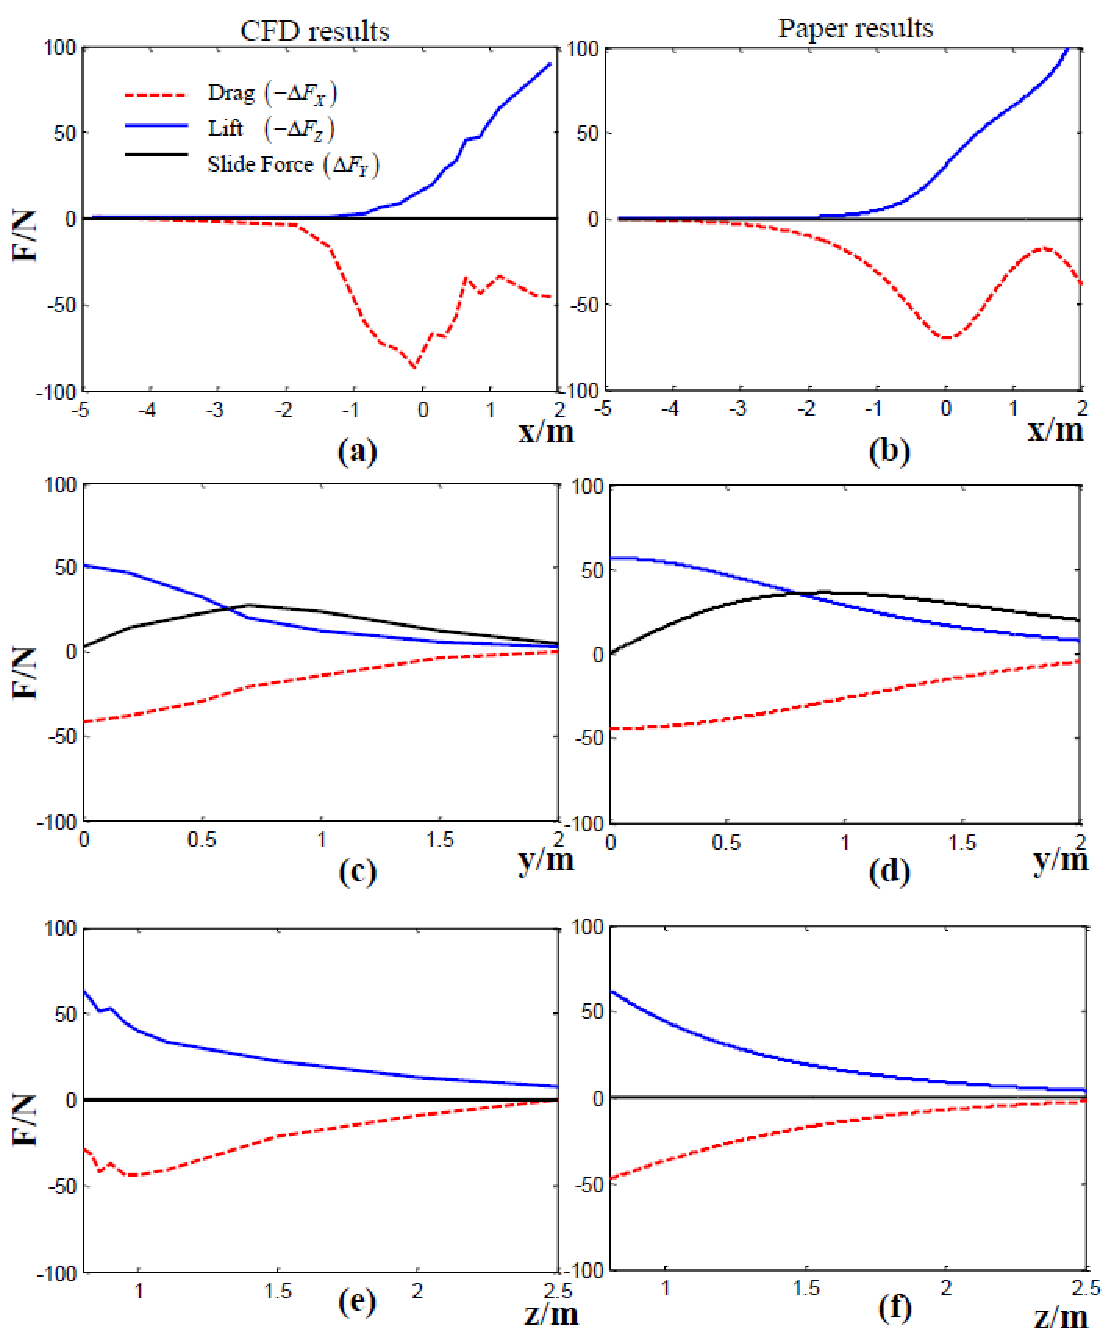
\includegraphics[width=0.8\textwidth]{Figures/Figs_Ch4/fig12.pdf}
	\caption{Validation of bow wave effect force model of the drogue against CFD results}\label{fig12}
\end{figure}
\clearpage
%\subsection{Assumption Verification}


%In order to facilitate the control design, the controlled plant is assumed to satisfy two assumptions.

%\textbf{Assumption 10.1}. Assume that ${{\mathbf{J}}_{0}} = {\mathbf{J}}\left( {{\mathbf{I}_3} + {{\mathbf{\Delta }}_{\text{J}}}} \right)$ with the uncertain matrix ${{\mathbf{\Delta }}_{\text{J}}}$ satisfying the following inequality:
%\begin{equation}\label{eq11}%yinyong\eqref{eq*}
%\underline{l}_{{{\text{J}}_\Delta }} \le \left\| {{{\mathbf{\Delta }}_\text{J}}} \right\| \le {{\bar{l}}_{{{\text{J}}_\Delta }}}, \left\| \frac{\partial {{{\mathbf{\Delta }}_\text{J}}}}{\partial t} \right\|\le {{l}_{{\text{J}_{t}}}}
%\end{equation}
%where $\underline{l}_{{{\text{J}}_\Delta }}>0$, ${{\bar{l}}_{{{\text{J}}_\Delta }}}>0$ , ${{l}_{{\text{J}_{t}}}}>0$. 


%\textbf{Assumption 10.2}. The unknown disturbance $\bm{\sigma }^{'}\left( t,\omega_{0} \right)$  satisfies the following inequalities:
%\begin{equation}\label{eq11a1}%yinyong\eqref{eq*}
%\left\| \bm{\sigma }^{'}\left( t,\omega_{0} \right) \right\|\le {{\delta }_{\sigma }}\left( t \right),  \left\| \frac{\partial \bm{\sigma }^{'}\left( t,\omega_{0} \right)}{\partial t} \right\|\le {{d}_{\sigma }}\left( t \right)
%\end{equation}
%where ${{\delta }_{\sigma }}\left( t \right)$, ${{d}_{\sigma }}\left( t \right)$ denote time-varying functions which have upper bounds ${{\bar{\delta }}_{\sigma }}$, ${\bar{d}_{\sigma }}$, respectively.

%\textit{Assumption 10.1} implies that ${{\mathbf{J}}^{ - 1}}{\mathbf{J}}_0=\mathbf{I}+{{\mathbf{\Delta }}_{\text{J}}}$. Then, $1+\underline{l}_{{{\text{J}}_\Delta }} \le \left\| {{{\mathbf{J}}^{ - 1}}{{\mathbf{J}}_0}} \right\| \le 1+{{\bar{l}}_{{{\text{J}}_\Delta }}}$. Furthermore, the inequality $\underline{l}_{{{\text{J}}_\Delta }} \le \left\| {{{\mathbf{J}}^{ - 1}}{{\mathbf{J}}_0} - {\mathbf{I}}} \right\| \le {{\bar{l}}_{{{\text{J}}_\Delta }}}$ is satisfied. Based on \textit{Assumptions 10.1-10.2}, $\bm{\sigma }\left( t,\omega_{0},\mathbf{x} \right)$ satisfies the following  inequalities:
%\begin{equation}\label{eq11a2}%yinyong\eqref{eq*}
%\begin{aligned}
%\left\| \bm{\sigma }\left( t,\omega_{0},\mathbf{x} \right) \right\|\le &  {{{k}}_{\sigma}}\left\| \mathbf{x} \right\|+{{\delta }_{\sigma }}\left( t \right),\\ 
%\left\| \frac{\partial \bm{\sigma }\left( t,\omega_{0},\mathbf{x} \right)}{\partial t} \right\|\le&  {{l}_{{{\sigma }_{t}}}}\left\| \mathbf{x} \right\|+{{d}_{\sigma }}\left( t \right), \\
%\left\| \frac{\partial \bm{\sigma }\left( t,\omega_{0},\mathbf{x} \right)}{\partial \mathbf{x}} \right\|= &\left\| ({{\mathbf{J}}^{-1}}{{\mathbf{J}}_{0}}-\mathbf{I }_3)\mathbf{{K}}^{\text{T}} \right\|\le {{{k}}_{\sigma}}\\
%\end{aligned}
%\end{equation}
%where ${{{k}}_{\sigma}}={{\bar{l}}_{{{\text{J}}_\Delta }}}\left\| \mathbf{K} \right\|$ and ${{l}_{{{\sigma }_{t}}}}={{l}_{{\text{J}_{t}}}}\left\| \mathbf{K} \right\|$ are positive constants. It is inferred from \eqref{eq87} that $\mathbf{h}\left( t,\mathbf{u} \right)={{\mathbf{J}}^{-1}}{{\mathbf{J}}_{0}}\mathbf{u}$, and ${{\partial {\mathbf{h}}\left( {t,{\mathbf{u}}} \right)} \mathord{\left/
%		{\vphantom {{\partial {\mathbf{h}}\left( {t,{\mathbf{u}}} \right)} {\partial {\mathbf{u}}}}} \right.
%		\kern-\nulldelimiterspace} {\partial {\mathbf{u}}}} = {{\mathbf{J}}^{ - 1}}{{\mathbf{J}}_0}$. Therefore,  $\mathbf{h}\left( t,\mathbf{u} \right)$ satisfies the following inequalities:
%\begin{equation}\label{eq24}%yinyong\eqref{eq*}
%1+\underline{l}_{{{\text{J}}_\Delta }} \le \left\| \frac{\partial \mathbf{h}\left( t,\mathbf{u} \right)}{\partial \mathbf{u}} \right\|\le 1+{{\bar{l}}_{{{\text{J}}_\Delta }}},\left\| \frac{\partial \mathbf{h}\left( t,\mathbf{u} \right)}{\partial t} \right\|\le {{l}_{{\text{J}_{t}}}}\left\| \mathbf{u} \right\|.
%\end{equation}	
%
%
%
%For simplicity of description, $\mathbf{h}\left( t,\mathbf{u} \right)$ is simplified as $\mathbf{h}$; $\bm{\sigma}\left( t,\omega_{0},\mathbf{x} \right)$ is simplified as $\bm{\sigma}$.  
%
%
%
%
%
%
%
%
%
%
%
%
%\section{Controller Design based on Additive-Output-Decomposition Framework}\label{sec4}%?3?
%
%\subsection{A Transformed Minimum-Phase System}\label{sec33}%?3?
%
%Since $\mathbf{{A}}$ is a Hurwitz matrix, according to \textit{Theorem 9.4} in \textit{Chapter 9}, there exists an output matrix $\mathbf{C}\in {\mathbb{R}^{6 \times 3}}$ as
%\begin{equation}\label{eq12a10}%yinyong\eqref{eq*}
%{{\mathbf{C}}^{\text{T}}}{\mathbf{A}} =  - {\mathbf{\Lambda }}{{\mathbf{C}}^{\text{T}}}
%\end{equation}
%where ${\mathbf{\Lambda }} = {\text{diag}}( 
%{{\lambda _1}}, {{\lambda_2}}, {{\lambda_3}} ) \in {\mathbb{R}^{3 \times 3}}$ is a diagonal matrix composed of positive real eigenvalues of ${{\mathbf{A}}^{\text{T}}}$. Let the output vector be defined as 
%\begin{equation}\label{eq12a8}%yinyong\eqref{eq*}
%\mathbf{y}={{\mathbf{C}}^{\text{T}}}\mathbf{x}.
%\end{equation}
%Based on \eqref{eq12a10}, and \eqref{eq12a8}, the first derivative of $\mathbf{y}$ along the solution to \eqref{eq86} is
%\begin{equation}\label{eq14}%yinyong\eqref{eq*}
%\mathbf{\dot{y}}=-\mathbf{\Lambda}\mathbf{ y}+{{\mathbf{C}}^{\text{T}}}\mathbf{B}{{\mathbf{v}}}
%\end{equation}
%where
%\begin{equation}\label{eq14a2}%yinyong\eqref{eq*}
%{{\mathbf{v}}}=\mathbf{h}-{{\mathbf{K}}^{\text{T}}}\mathbf{x}+\bm{\sigma}. 
%\end{equation}
%Notice that the output $\mathbf{y}$ only contains part of elements (the output vector $\mathbf{y}$ has 3 elements) in all states (the state vector $\mathbf{x}$ has $6$ elements ${{x}_{1}},{{x}_{2}},...,{{x}_{6}}$).  Therefore, the remaining 3 state equations are expressed as \cite[pp. 351]{Hassan2011non}
%\begin{equation}\label{eq15}%yinyong\eqref{eq*}
%\bm{\dot{\eta }}={{\mathbf{A}}_{\eta }}\bm{\eta }+{{\mathbf{B}}_{\eta }}\mathbf{y }
%\end{equation}
%where $\bm{{\eta }}\in {\mathbb{R}^{3}}$ is an internal state vector, ${{\mathbf{A}}_{\eta }}\in {\mathbb{R}^{3 \times 3}}$ and ${{\mathbf{B}}_{\eta }}\in {\mathbb{R}^{3 \times 3}}$ are constant matrices. According to \eqref{eq14} and \eqref{eq15}, \eqref{eq86} is expressed in the form of a block matrix \cite{Quan1}:
%\begin{equation}\label{eq15a1}%yinyong\eqref{eq*}
%\left[ \begin{matrix}
%{\bm{\dot{\eta }}}  \\
%{\mathbf{\dot{y}}}  \\
%\end{matrix} \right]={{\mathbf{\bar{A}}}}\left[ \begin{matrix}
%\bm{\eta }  \\
%\mathbf{y}  \\
%\end{matrix} \right]+\left[ \begin{matrix}
%{{\mathbf{0}}_{3\times 3}}  \\
%{{\mathbf{C}}^{\text{T}}}\mathbf{B}  \\
%\end{matrix} \right]{{\mathbf{v}}}
%\end{equation}
%where ${{{\mathbf{\bar{A}}}}}=\left[ \begin{matrix}
%{{\mathbf{A}}_{\eta }} & {{\mathbf{B}}_{\eta }}  \\
%{{\mathbf{0}}_{3\times  3 }} & -\mathbf{\Lambda }  \\
%\end{matrix} \right]$. Because ${{{\mathbf{\bar{A}}}}}$ is an upper triangular matrix, and the eigenvalues of ${{\mathbf{A}}_{\eta }}$ are all from $\mathbf{{A}}$. Therefore, ${{\mathbf{A}}_{\eta }}$ is a Hurwitz matrix, namely, the internal dynamics \eqref{eq15} is stable.  If $\mathbf{y}\to \mathbf{0}$, then ${\bm{{\eta }}}\to \mathbf{0}$ and then  $\mathbf{x}\to \mathbf{0}$ according to \eqref{eq15}. This implies that  \eqref{eq15a1} with $\mathbf{y}$ as output is a minimum-phase system. Therefore, the next step is to design the control signal $\mathbf{u}$ making the output $\mathbf{y}$ gradually converge to zero. This is only a motivation to design. A formal proof will be give in \textit{Theorem 10.1}.
%
%\subsection{Controller Design}
%
%The dynamic equation \eqref{eq14} is viewed as the original system \cite{Quan6}, and then the primary system is designed as
%\begin{equation}\label{eq16}%yinyong\eqref{eq*}
%{{{\mathbf{\dot{y}}}}_{\text{p}}}=-\mathbf{\Lambda}{{\mathbf{y}}_{\text{p}}}+{{\mathbf{C}}^{\text{T}}}\mathbf{Bu},{{\mathbf{y}}_{\text{p}}}\left( \mathbf{0} \right)=\mathbf{0} \\ 
%\end{equation}
%where ${{\mathbf{y}}_{\text{p}}}\in {{\mathbb{R} }^{3}}$ denotes the state of the primary system. Based on the additive-output-decomposition-based control framework \cite{Quan2}, the secondary system is equal to the original system minus the primary system:
%\begin{equation}\label{eq16a3}%yinyong\eqref{eq*}
%\begin{aligned}
%\mathbf{\dot{y}}-{{{\mathbf{\dot{y}}}}_{\text{p}}}=&{{\mathbf{C}}^{\text{T}}}\mathbf{B}\mathbf{v}-\mathbf{\Lambda}\mathbf{y}+\mathbf{\Lambda}{{\mathbf{y}}_{\text{p}}}-{{\mathbf{C}}^{\text{T}}}\mathbf{Bu}. \\ 
%\end{aligned}
%\end{equation}
%The state of secondary system ${{\mathbf{y}}_{\text{s}}}\in {{\mathbb{R} }^{3}}$ is defined as:
%\begin{equation}\label{eq16a1}%yinyong\eqref{eq*}
%{{\mathbf{{y}}}_\text{s}}=\mathbf{{y}}-{{\mathbf{{y}}}_{\text{p}}}
%\end{equation}
%where ${{\mathbf{y}}_\text{s}}\left( \mathbf{0} \right)={\mathbf{C}}^{\text{T}}\mathbf{x}_0$. 
%Following the controller design in \textit{Table 1 }of \textit{Chapter 9}, an additive-output-decomposition-based dynamic inversion controller is designed as follows:
%\begin{equation}\label{eq19a2}%yinyong\eqref{eq*}
%\mathbf{u}_\text{PI}\left( s \right)=-\frac{1}{\epsilon }{{\left( {{\mathbf{C}}^{\text{T}}}\mathbf{B} \right)}^{-1}}{{\mathbf{C}}^{\text{T}}}\mathbf{x}\left( s \right)-\frac{1}{\epsilon s}\mathbf{\Lambda }{{\left( {{\mathbf{C}}^{\text{T}}}\mathbf{B} \right)}^{-1}}{{\mathbf{C}}^{\text{T}}}\mathbf{x}\left( s \right).
%\end{equation}
%However, there are not only low-frequency disturbances but also vibration components related to the angular velocity of propellers in the quadcopter. Therefore, $\mathbf{Q}\left( s \right)$ is designed as follows:
%\begin{equation}\label{eq20}%yinyong\eqref{eq*}
%\mathbf{Q}\left( s \right)=\frac{1}{\epsilon s+1}\mathbf{I}_3+{Q}_{\omega }\mathbf{I}_3
%\end{equation}
%%$\mathbf{Q}\left( s \right)=\frac{1}{\epsilon s+1}\mathbf{I}_m+\frac{\left( {{\omega }_{0}}/q %\right)s}{{{s}^{2}}+\left( {{\omega }_{0}}/q \right)s+\omega _{0}^{2}}\mathbf{I}_m$
%where ${Q}_{\omega }=\frac{\left( {{\omega }_{0}}/q \right)s}{{{s}^{2}}+\left( {{\omega }_{0}}/q \right)s+\omega _{0}^{2}}$ is a band-pass filter, and $q$ represents the quality factor; $\omega_{0}$ is the dominant frequency.  Substituting the new filter \eqref{eq20} into \eqref{eq19a2} yields the proposed controller:
%\begin{equation}\label{eq19a5}%yinyong\eqref{eq*}
%\begin{aligned}
%{\mathbf{u}}\left( s \right) ={{\mathbf{u}}_{{\text{PI}}}}\left( s \right)+ \mathbf{u}_\omega\left( s \right) \\ 
%\end{aligned} 
%\end{equation}
%where 
%\begin{equation}\label{eq19a6}%yinyong\eqref{eq*}
%\mathbf{u}_\omega\left( s \right)=-\left( s{{\mathbf{I}}_{3}}+\mathbf{\Lambda } \right){{\left( {{\mathbf{C}}^{\text{T}}}\mathbf{B} \right)}^{-1}}\frac{\left( {{\omega }_{0}}/q \right)s}{{{s}^{2}}+\omega _{0}^{2}}{{\mathbf{C}}^{\text{T}}}\mathbf{x}\left( s \right).
%\end{equation}
%Whether to introduce the term $\mathbf{u}_\omega\left( s \right)$ is determined according to the characteristics of external disturbance (vibration noise). If no particular frequency vibration is detected, set $\omega_0=0$, that is, $\mathbf{u}_\omega$ does not work. Only when the sensor detects the presence of a specific frequency component $\omega_0$ (such as vibration) in the closed-loop system.  Then, $\mathbf{u}_\omega$ is incorporated into $\mathbf{u}$, and the performance of suppressing disturbance is expected to be significantly enhanced.
%
%
%\subsection{Stability and Performance Analysis}\label{sec6}%?3?
%
%
%
%Recalling \eqref{eq20}, if $s=0,$ $\mathbf{I}_3-\left.\mathbf{Q}\left(s\right)\right\vert _{s=0}$ equal to
%\begin{align*}
%& \mathbf{I}_3-\left.\frac{1}{\epsilon s+1}\mathbf{I}_3\right\vert _{s=0}-\left.\frac{\left(\omega_{0}\left/q\right.\right)s}{s^{2}+\left(\omega_{0}\left/q\right.\right)s+\omega_{0}^{2}}\mathbf{I}_3\right\vert _{s=0}\\
%& =\mathbf{I}_3-\mathbf{I}_3-{{\mathbf{0}}_{3\times 3}}\\
%& ={{\mathbf{0}}_{3\times 3}}.
%\end{align*}
%If $s=j\omega_{0},$ since $\omega_{0}\gg0,$ $\mathbf{I}_3-\left.\mathbf{Q}\left(s\right)\right\vert _{s=j\omega_{0}}$ equal to
%\begin{align*}
%& \mathbf{I}_3-\left.\frac{1}{\epsilon s+1}\mathbf{I}_3\right\vert _{s=j\omega_{0}}-\left.\frac{\left(\omega_{0}\left/q\right.\right)s}{s^{2}+\left(\omega_{0}\left/q\right.\right)s+\omega_{0}^{2}}\mathbf{I}_3\right\vert _{s=j\omega_{0}}\\
%& \approx \mathbf{I}_3-{{\mathbf{0}}_{3\times 3}}-\mathbf{I}_3\\
%& ={{\mathbf{0}}_{3\times 3}}.
%\end{align*}
%Therefore, it is expected that the newly designed filter \eqref{eq20} can simultaneously suppress low-frequency disturbances and a frequency component around $\omega_{0}$. The bigger the value of $q$ is, the more pronounced the filter effect has. Before proceeding further, an assumption on the lumped disturbance ${{\mathbf{d}}_\text{l}}$ is imposed.
%
%\textbf{Assumption 10.3}. There exists the  Laplace transform of ${{\mathbf{d}}_\text{l}}$. 
%
%According to \textit{Assumption 10.3}, the  Laplace transform of the lumped disturbance $\mathbf{d}_\text{l}$ is given as follows:
%\begin{equation}\label{eq25a3}%yinyong\eqref{eq*}
%\begin{aligned}
%{{\mathbf{d}}_\text{l}}\left( s \right)=-\mathbf{G}\left( s \right)\mathbf{u}\left( s \right)+{{\left( s{{\mathbf{I}}_{3}}+\mathbf{\Lambda } \right)}^{-1}}{{\mathbf{C}}^{\text{T}}}{{\mathbf{x}}_{0}}+\mathbf{G}\left( s \right) \mathbf{v}\left( s \right). 
%\end{aligned}
%\end{equation}
%Substituting \eqref{eq25a3} into (40) of \textit{Chapter 9}, then, the control signal can be further denoted as
%\begin{equation}\label{eq25a4b}%yinyong\eqref{eq*}
%\begin{aligned}
%\mathbf{u}\left( s \right)=&-\left( \frac{1}{\epsilon s+1}+{{Q}_{\omega }} \right){{\left( {{\mathbf{C}}^{\text{T}}}\mathbf{B} \right)}^{-1}}{{\mathbf{C}}^{\text{T}}}{{\mathbf{x}}_{0}} \\ 
%& -\left( \frac{1}{\epsilon s+1}+{{Q}_{\omega }} \right)\left( \mathbf{v}\left( s \right)-\mathbf{u}\left( s \right) \right). \\ 
%\end{aligned}
%\end{equation}
%Since $-{{\left( {{\mathbf{C}}^{\text{T}}}\mathbf{B} \right)}^{-1}}{{\mathbf{C}}^{\text{T}}}{{\mathbf{x}}_{0}}$ is a constant value signal, its inverse Laplace transform is an impulse signal, and will vanish. Therefore, for simplicity, \eqref{eq25a4b} is considered as
%\begin{equation}\label{eq25a4b3}%yinyong\eqref{eq*}
%\mathbf{u}\left( s \right)=-\left( \frac{1}{\epsilon s+1}+{{Q}_{\omega }} \right)\left( \mathbf{v}\left( s \right)-\mathbf{u}\left( s \right) \right). 
%\end{equation}
%The poles of ${Q}_{\omega }$ are taken to study its frequency characteristics. Let the denominator of ${Q}_{\omega }$ equal zero, namely, ${{{s}^{2}}+\left( {{\omega }_{0}}/q \right)s+\omega _{0}^{2}}=0$. Then, the following characteristic roots are obtained as
%\begin{equation}\label{eq25a5b2}%yinyong\eqref{eq*}
%{{s}_{1}}=\frac{-{{\omega }_{0}}+{{\omega }_{0}}\sqrt{1-4{{q}^{2}}}}{2q},{{s}_{2}}=\frac{-{{\omega }_{0}}-{{\omega }_{0}}\sqrt{1-4{{q}^{2}}}}{2q}.
%\end{equation}
%In the real experiment, it is found that the average angular frequency of each propeller is about 99.06 Hz. If these design parameters $q=0.5$, ${\omega }_{0}=$100Hz are chosen, then a higher decay rate is obtained (${{s}_{1}}={{s}_{2}}=-100$). Namely, the term $\mathbf{v}\left( s \right)-\mathbf{u}\left( s \right) $  will rapidly decay to 0. For the sake of analysis, \textit{Assumption 10.4} is introduced. 
%
%\textbf{Assumption 10.4}. There exist ${{\bar{\delta }}_{q}}>0$ and $T_0>0$ such that
%\begin{equation}\label{eq12a11}%yinyong\eqref{eq*}
%\mathcal{L}^{-1}\left((\epsilon s+1){Q}_{\omega }\left( \mathbf{v}\left( s \right)-\mathbf{u}\left( s \right) \right)\right)= {{\bm{\delta }}_{q}}(t)\left(\mathbf{v}\left( t \right)-\mathbf{u}\left( t \right)\right)
%\end{equation}
%where ${{\bm{\delta }}_{q}}(t)\in {\mathbb{R}^{3\times 3}}$ is a matrix function, and $\left\| {\bm{\delta }_{q}}(t) \right\|\le {{\bar{\delta }}_{q}}$ after $t>T_0$. 
%
%
%Based on \textit{Assumption 10.4}, the inversion Laplace transform of \eqref{eq25a4b} is rewritten as
%\begin{equation}\label{eq25a1b}%yinyong\eqref{eq*}
%\epsilon\mathbf{\dot{u}}=-\left( {1 + \bm{\delta} _q} \right)\mathbf{v}+{{\bm{\delta }}_{q}}\mathbf{u}.
%\end{equation}
%In the following, \textit{Theorem 10.1} and \textit{Corollary 10.1} are proposed to show that $\mathbf{u}_\text{PI}+\mathbf{u}_\omega$ not only can attenuate noise at a specific frequency but also guarantee the state $\mathbf{y}$ can converge to the neighborhood near the origin.
%
%
%\textbf{Theorem 10.1.} Suppose that 1) \textit{Assumptions 10.1-10.4} hold, 2) the controller is designed as \eqref{eq19a5} with $\mathbf{Q}\left( s \right)$ shown in \eqref{eq20}, 3) matrix ${{\mathbf{C}}^{\text{T}}}\mathbf{B}$ is invertible. If the involved parameter $\epsilon$ satisfies the following inequality:
%\begin{equation}\label{eq25a11}%yinyong\eqref{eq*}
%0<\epsilon <\frac{4(1+\underline{l}_{{{\text{J}}_\Delta }}){{\gamma }_{1}}}{2{{\gamma }_{1}}{{\gamma }_{2}}+\gamma _{3}^{2}}
%\end{equation}
%where 
%\begin{align*}
%\begin{aligned}
%{{\gamma }_{1}}=& {{\lambda }_{\min }}\left( \mathbf{M} \right) \\ 
%{{\gamma }_{2}}=& 2\left( \left\| \mathbf{K} \right\|+{k_\sigma } \right)\left\| \mathbf{B} \right\|-(1+\underline{l}_{{{\text{J}}_\Delta }})2\left( 1+{{{\bar{\delta }}}_{q}} \right) \\& +2\left(\frac{{{l}_{{\text{J}_{t}}}}}{1+{{\bar{l}}_{{{\text{J}}_\Delta }}} }+ {{\bar \delta }_q} \right) + \frac{1+\underline{l}_{{{\text{J}}_\Delta }}}{\epsilon }  \\
%{{\gamma }_{3}}=& 2\left\| \mathbf{B} \right\|\left\| \mathbf{P} \right\|+2\left( \left\| \mathbf{K} \right\|+{k_\sigma } \right)\left\| \mathbf{A} \right\|  + 2{l_{{\sigma _t}}}\\& + 2\left(\frac{{{l}_{{\text{J}_{t}}}}}{1+{{\bar{l}}_{{{\text{J}}_\Delta }}} }+ {{\bar \delta }_q} \right)(1+{{\bar{l}}_{{{\text{J}}_\Delta }}}) \left( {\left\| {\mathbf{K}} \right\| + {k_\sigma }} \right) \\ 
%\end{aligned}
%\end{align*}
%and matrices $\mathbf{P}$ and $\mathbf{M}$ satisfies \eqref{eq12a1}. Then, the closed-loop system is globally uniformly ultimately bounded. 
%
%Proof. See \textit{Appendix \ref{sec91}}. $\square$
%
%\textbf{Corollary 10.1} Suppose that conditions of \textit{Theorem 10.1} hold, and \eqref{eq86} is degraded into the following linear system \eqref{eq25a7} with $\bm{\sigma} \left(t,\omega_{0} \right)$ having only constant and specific frequency ${\omega }_{0}$ components:
%\begin{equation}\label{eq25a7}%yinyong\eqref{eq*}
%\begin{aligned}
%& \mathbf{\dot{x}}\left( t \right)={{\mathbf{A}}_{0}}\mathbf{x}\left( t \right)+\mathbf{B}\left( \left( {{\mathbf{I}}_{3}}+{{\mathbf{\Delta }}_{h}} \right)\mathbf{u}+\bm{\sigma }\left(t, \omega_{0} \right) \right) \\ 
%& \mathbf{x}\left( 0 \right)={{\mathbf{x}}_{0}} \\ 
%\end{aligned}
%\end{equation}
%where ${{\mathbf{\Delta }}_{h}}\in {\mathbb{R}^{3\times 3}}$. Then $\underset{t\to \infty }{\mathop{\lim }}\,\left\|\mathbf{x}(t) \right\|=0$, namely, all states approach to zero. 
%
%
%Proof. See \textit{Appendix \ref{sec92}}. $\square$
%
%\subsection{Controller Discretization}
%The proposed controller \eqref{eq19a5} is further rewritten as
%\begin{equation}\label{eq19a5b}%yinyong\eqref{eq*}
%{\mathbf{u}}\left( s \right) = {{\mathbf{G}}_{\text{B}}}\left( s \right){\mathbf{x}}\left( s \right)
%\end{equation}
%where ${\mathbf{x}}\left( s \right)$ is viewed as the input signal; ${{\mathbf{G}}_{\text{B}}}\left( s \right)$ denotes the transfer function from ${\mathbf{x}}\left( s \right)$ to ${\mathbf{u}}\left( s \right)$. In order to make the proposed controller realizable by a digital computer, the designed  ${{\mathbf{G}}_{\text{B}}}\left( s \right)$ should be discretized. The classical Tustin discretization method is used as
%\begin{equation}
%\mathbf{D}_{{z}}{{(z)=\left. {{\mathbf{G}}_{\text{B}}}\left( s \right)\right\vert }_{s=\frac{2}{T}\frac{{z-1}}{{z+1}}}}
%\label{39}
%\end{equation}%
%where $\mathbf{D}_{z}(z)$ denotes the digital transfer function; $z$ denotes the discretization transform symbol; $T$ is the sampling period. However, the classical Tustin method is prone to frequency aliasing and cannot filter out signals of specified frequencies. To obtain a good vibration suppression effect, the proposed controller needs to accurately filter out the disturbance signal at a specified frequency. Therefore, the following Tustin transformation with the prewarping discretization method \cite[p. 243]{aastrom2013computer} is used:
%\begin{equation}
%\mathbf{D}_{{z}}{{(z)=\left. {{\mathbf{G}}_{\text{B}}}\left( s \right)\right\vert }_{s = \frac{{{\omega _0}}}{{\tan (\frac{{{\omega _0}T}}{2})}}\frac{{z - 1}}{{z + 1}}}}  \label{43}
%\end{equation}%
%where $\omega_{0} $ is the dominant frequency also the notch frequency.
%
%\section{Experiment Verification}\label{sec66}%?3?
%
%In this section, a practical experiment is provided to illustrate that the proposed control algorithm has a stronger vibration suppression capability compared to the traditional additive-output-decomposition dynamic inversion controller. The detailed experimental process can be found in the video at $http://rfly.buaa.edu.cn/$ (Click the 'Videos Demonstration' button).
%
%
%
%\subsection{Introduction to Experiment Platform}\label{sec661a}%?3?
%\begin{figure}[th]
%	\centering
%	\includegraphics[width=0.7\textwidth]{Chap10/fig4_hardware.pdf}
%	\caption{Simulation procedure \cite{WangS}}\label{Hardware}
%\end{figure}
%\begin{figure}[th]
%	\centering
%	\includegraphics[width=0.7\textwidth]{Chap10/fig5_X_type_quadcopter.pdf}
%	\caption{A laser fixed to an X-type quadcopter pointing to a target}\label{realquadcopter}
%\end{figure}
%
%
%This experiment adopts a professional experiment platform provided by \cite{WangS}. As shown in Fig. \ref{Hardware},  the whole experimental platform is divided into two parts: an SIL simulation and a flight experiment. In the controller design phase,  the Simulink software  is used to construct the proposed controller and the complete quadcopter model. Then, the SIL simulation block is performed such that the control parameters are  preliminarily tuned. Next, the controller in Simulink is converted into C++ language. Finally, a flight experiment is performed to verify the vibration suppression capability of the proposed control algorithm. 
%
%As shown in Fig. \ref{realquadcopter}, this experiment takes an X-type quadcopter as the controlled plant, and its parameters are shown in Table \ref{Tab_9-1}.
%
%
%\subsection{Controller Design}\label{sec661}%?3?
%
%According to \eqref{eq19a5}, the controller is designed as
%\begin{equation}\label{eq90}%yinyong\eqref{eq*}
%\begin{aligned}
%{{u }_{\phi }}=& -\frac{1}{{{\epsilon }_{\phi }}}{{\left( \mathbf{C}_{\phi }^{\text{T}}{{\mathbf{B}}}_{0} \right)}^{-1}}\mathbf{C}_{\phi }^{\text{T}}{{\mathbf{x}}_{\phi }}\left( s \right)-\frac{1}{{{\epsilon }_{\phi }}s}{{\mathbf{\Lambda }}_{\phi }}{{\left( \mathbf{C}_{\phi }^{\text{T}}{{\mathbf{B}}}_{0} \right)}^{-1}}\mathbf{C}_{\phi }^{\text{T}}{{\mathbf{x}}_{\phi }}\left( s \right) \\ 
%& -\left( s\mathbf{I}+{{\mathbf{\Lambda }}_{\phi }} \right){{\left( \mathbf{C}_{\phi }^{\text{T}}{{\mathbf{B}}}_{0} \right)}^{-1}}\frac{\left( {{\omega }_{0}}/{{q}} \right)s}{{{s}^{2}}+\omega _{0}^{2}}\mathbf{C}_{\phi }^{\text{T}}{{\mathbf{x}}_{\phi }}\left( s \right) \\ 
%{{u }_{\theta }}=& -\frac{1}{{{\epsilon }_{\theta }}}{{\left( \mathbf{C}_{\theta }^{\text{T}}{{\mathbf{B}}}_{0} \right)}^{-1}}\mathbf{C}_{\theta }^{\text{T}}{{\mathbf{x}}_{\theta }}\left( s \right)-\frac{1}{{{\epsilon }_{\theta }}s}{{\mathbf{\Lambda }}_{\theta }}{{\left( \mathbf{C}_{\theta }^{\text{T}}{{\mathbf{B}}}_{0} \right)}^{-1}}\mathbf{C}_{\theta }^{\text{T}}{{\mathbf{x}}_{\theta }}\left( s \right) \\ 
%& -\left( s\mathbf{I}+{{\mathbf{\Lambda }}_{\theta }} \right){{\left( \mathbf{C}_{\theta }^{\text{T}}{{\mathbf{B}}}_{0} \right)}^{-1}}\frac{\left( {{\omega }_{0}}/{{q}} \right)s}{{{s}^{2}}+\omega _{0}^{2}}\mathbf{C}_{\theta }^{\text{T}}{{\mathbf{x}}_{\theta }}\left( s \right) \\ 
%{{u }_{\psi }}=& -\frac{1}{{{\epsilon }_{\psi }}}{{\left( \mathbf{C}_{\psi }^{\text{T}}{{\mathbf{B}}}_{0} \right)}^{-1}}\mathbf{C}_{\psi }^{\text{T}}{{\mathbf{x}}_{\psi }}\left( s \right)-\frac{1}{{{\epsilon }_{\psi }}s}{{\mathbf{\Lambda }}_{\psi }}{{\left( \mathbf{C}_{\psi }^{\text{T}}{{\mathbf{B}}}_{0} \right)}^{-1}}\mathbf{C}_{\psi }^{\text{T}}{{\mathbf{x}}_{\psi }}\left( s \right) \\ 
%& -\left( s\mathbf{I}+{{\mathbf{\Lambda }}_{\psi }} \right){{\left( \mathbf{C}_{\psi }^{\text{T}}{{\mathbf{B}}}_{0} \right)}^{-1}}\frac{\left( {{\omega }_{0}}/{{q}} \right)s}{{{s}^{2}}+\omega _{0}^{2}}\mathbf{C}_{\psi }^{\text{T}}{{\mathbf{x}}_{\psi }}\left( s \right) \\ 
%\end{aligned}
%\end{equation}
%where $\mathbf{C}_{\phi}\in {\mathbb{R}^{2}}, \mathbf{C}_{\theta}\in {\mathbb{R}^{2}}, \mathbf{C}_{\psi}\in {\mathbb{R}^{2}}$, $\epsilon_{\phi}, \epsilon_{\theta}, \epsilon_{\psi}$, $\mathbf{\Lambda }_{\phi}, \mathbf{\Lambda }_{\theta}, \mathbf{\Lambda }_{\psi}$ are design parameters. The roll channel is taken as an example to introduce the design process of the proposed controller, while the design process of the pitch and yaw channels is the same.
%
%(1) Proposed controller (PI controller with a notch filter):
%
%Step 1: Choose following desired closed-loop poles $-1.4, -5$. Next, obtain the state feedback gain matrix $\mathbf{K}_{\phi }={{\left[ \begin{matrix}
%		-0.0453 & -0.0414  \\
%		\end{matrix} \right]}^{\text{T}}}$   resulting in $\mathbf{A}_{\phi}=\mathbf{\bar{A}}_{0}+\mathbf{B}_{0}\mathbf{K}_{\phi }^{\text{T}}$ by pole configuration. 
%
%Step 2: Choose eigenvalues of $\mathbf{A}_{\phi}^{\text{T}}$ corresponding to its eigenvalue -1.4 ($\mathbf{\Lambda }_{\phi}=1.4$) results in $\mathbf{C}_{\phi}={{\left[ \begin{matrix}
%		0.9806 & 0.1961   \\
%		\end{matrix} \right]}^{\text{T}}}$.  Obviously ${{\mathbf{C}_{\phi}}^{\text{T}}}\mathbf{B}_{0}\ne \mathbf{0}$.
%
%Step 3: The proposed controller is designed as \eqref{eq19a5}.
%
%
%Step 4: Design the the following control parameters: $\epsilon_{\phi}=0.1 $, $q=50$, $\omega_{0}=99.06$.
%
%For pitch, and yaw channel, the proposed controller choose the same control parameters. For a fair comparison, the PI controller with similar parameters is designed according to \cite{Quan1}.
%
%(2) Existing controller \cite{Quan1} (PI controller):  The design steps for this existing controller are the same as for the proposed controller.  Only the controller as described in \eqref{eq19a2} is used, so it has only one control parameter $\epsilon_{\phi}=0.1 $.
%\begin{table}[th]
%	\caption{Parameters of the experimental quadcopter}
%	\renewcommand\arraystretch{1.3}
%	\centering
%	\begin{tabular}	
%		[c]{|c|c|c|c|}
%		
%		\hline
%		Total mass ${m}$ & 1.09 kg  & Airframe radius $d$ & 0.165 m
%		\\\hline 
%		Motor brand & KV800 & Motor bandwidth ${{T}_{\text{m}}}$ & 50
%		\\\hline
%		Propeller brand & DJI 8045 & X-inertia ${{J}_{\phi }}$ (kg.$\text{m}^2$)  & 6.47${e^{ - 3}}$ 
%		\\\hline
%		Battery brand & LiPo 3S & Y-inertia ${{J}_{\theta }}$ (kg.$\text{m}^2$)  & 6.47${e^{ - 3}}$
%		\\\hline
%		Rotor inertia & $1.287{e^{ - 4}}$ & Z-inertia ${{J}_{\psi }}$ (kg.$\text{m}^2$) & 1.227${e^{-2}}$
%		\\\hline
%		ESC brand &  Hobbywing & Gravity acceleration \text{g} & 9.81 ${{\text{m}} \mathord{\left/
%				{\vphantom {{\text{m}} {{{\text{s}}^2}}}} \right.
%				\kern-\nulldelimiterspace} {{{\text{s}}^2}}}$
%		\\\hline
%		Torque coefficient $c_\text{T}$ &  $5.234{e^{-8}}$  & Thrust coefficient $c_\text{M}$ & $8.824{e^{ - 6}}$ 
%		\\\hline
%		Unbalanced  mass $m_i^u$ &  $2.75{e^{-7}}$ kg & Additional offset $r_i^u$ & $9.9{e^{ - 2}}\text{m}$
%		\\\hline
%	\end{tabular}
%	\label{Tab_9-1}
%\end{table}
%\subsection{SIL Simulation}\label{sec662}%?3?
%
%The sampling period of the SIL simulation is set to 0.004s. Driven by the existing controller, the experimental results are shown in Figs. \ref{angle}-\ref{FIG_7}.  Figs. \ref{angle}-\ref{angle_rate} show attitude angle curves and attitude angle rate curves, respectively.  Although attitude angle rate curves converge to zero, these curves are not very smooth. Because there exists high-frequency noise related to the angular frequency of the propeller. Therefore, it is necessary to introduce a notch filter in the existing PI controller to eliminate the high-frequency noise, which is one of the innovations of this controller.  Fig. \ref{FIG_6} shows that the mean angular velocity of all propellers is approximately 621.8 rad/s.    For the PI controller, the black dashed line in Fig. \ref{FIG_7} shows the vibration spectrum of $\dot{\omega }_\phi$. It is observed that the  peak of the vibration spectrum is concentrated around the frequency of 99.06Hz (621.8rad/s), and the amplitude reaches 17.89. Since the peak frequency is very close to the frequency propellers rotating, it implies that the vibration is mainly caused by the unbalanced mass of the propeller, which seriously affects the stability of the attitude.
%
%\begin{figure}[th]
%	\centering
%	\includegraphics[width=0.6\textwidth]{Chap10/fig6_roll_angle.pdf}
%	\caption{Attitude angle output in SIL simulation}\label{angle}
%\end{figure}
%
%\begin{figure}[th]
%	\centering
%	\includegraphics[width=0.6\textwidth]{Chap10/fig7_roll_angle_rate.pdf}
%	\caption{Attitude angle rate output in SIL simulation}\label{angle_rate}
%\end{figure}
%
%\begin{figure}[th]
%	\centering
%	\includegraphics[width=0.6\textwidth]{Chap10/fig8_propeller_velocity.pdf}
%	\caption{Angular speed of each propeller in SIL simulation}\label{FIG_6}
%\end{figure}
%
%\begin{figure}[th]
%	\centering
%	\includegraphics[width=0.6\textwidth]{Chap10/fig9_spectrum_roll_rate.pdf}
%	\caption{Vibration spectrum of $\dot{\omega }_\phi$ under different controllers in SIL simulation}\label{FIG_7} 
%\end{figure}
%
%
%\begin{figure}[th]
%	\centering
%	\includegraphics[width=0.6\textwidth]{Chap10/fig10_lisan.pdf}
%	\caption{Vibration spectrum of $\dot{\omega }_\phi$ of proposed controller under different discretization in SIL simulation}\label{FIG_8}
%\end{figure}
%
%
%In order to suppress the vibration signal of this specific frequency, additional control signal $\mathbf{u}_\omega\left( s \right)$ is then introduced, namely the  proposed controller. The term $\mathbf{u}_\omega\left( s \right)$ has the following control parameters:  ${\omega }_{0}$, $q$. The parameter ${\omega }_{0}$ is mainly determined by the angular velocity corresponding to the peak frequency. Therefore, parameter ${\omega }_{0}$ is selected as ${\omega }_{0}=99.06$ Hz. The bigger the value of the quality factor $q$ is, the more obvious the suppression ability has, but the lower the stability margin of the closed-loop system has.  In order to balance the robustness and suppression ability of the the closed-loop system, the quality factor $q$, in this chapter, is chosen as 50. As shown by the solid red line in Fig. \ref{FIG_7}, the vibration spectrum for $\dot{\omega }_\phi$ is more uniformly distributed over the frequency range, driven by the proposed controller. For the proposed controller with the Tustin discretization method, the peak appears at frequency 99.16Hz, which is attenuated by $1-4.774/17.89=73.31\%$.
%
%Notice that the designed controller for the quadcopter is discretized by prewarping Tustin transformation.  This discretization method can accurately suppress the peak  amplitude in a specific frequency range.  The peak magnitude is proportional to the magnitude of the disturbance.  For example, when 99.16Hz is used as the parameter of the prewarping Tustin transformation algorithm, the spectral peak of the roll channel is significantly reduced compared with the Tustin discretization method.  The detailed simulation results are shown in Fig. \ref{FIG_8}, and  the peak is attenuated by $1-2.118/4.774=55.63\%$. Therefore, the prewarping Tustin transformation will be used to discrete the proposed controller in the following experiment. Compared with the PI controller,  the peak is attenuated by $1-2.118/17.89=88.16\%$.
%
%
%
%\subsection{Flight Experiment}\label{sec663}%?3?
%The experimental environment is set as follows: Operating System (OS): Windows 10, 64-bit system; Processor: Intel(R) Core(TM) i7-9750H CPU @ 2.60GHz; Memory: 16G; Software: MATLAB 2017b; Autopilot: Pixhawk 2; Remote controller: RadioLink AT9S; Sampling period: 0.004s. A scissor is used to cut a tenth of the left propeller to get a unbalanced propeller. The whole experimental procedure is divided into the following steps:
%
%Step 1. Use the PI controller to control the attitude of the quadcopter and let it at a hovering phase in the air for tens of seconds, recording the average angular frequency of each propeller.  
%
%Step 2. Take the mean angular frequency of four propellers as the designed parameter ${\omega }_{0}$ of the notch filter.
%
%Step 3. Use the proposed controller with a notch filter to control the attitude of the quadcopter. Let the quadcopter take off in the self-stabilizing mode and record the angle acceleration information. 
%
%\begin{figure}
%	\centering
%	\includegraphics[width=0.7\textwidth]{Chap10/fig11_ch10.pdf}
%	\caption{Vibration spectrum of the $\dot{\omega }_\phi$ under different controllers in real experiment}\label{Experimentnew}
%\end{figure}
%
%
%After completing \textit{Step 1}, the mean angular frequency of the propeller was tested to be about 100 Hz. Therefore, the parameter ${\omega }_{0}$ is designed as 100. Next, collect the data of the quadcopter in the hover mode and perform spectrum analysis to obtain the results shown in Figs. \ref{Experimentnew}. As shown by the solid red line in Fig. \ref{Experimentnew}(b), the vibration spectrum for $\dot{\omega }_\phi$ is more uniformly distributed over the frequency range, driven by the proposed controller. For the PI controller \cite{Quan1}, the peak is concentrated around the frequency of 99.4Hz, and the peak amplitude reaches 8.598, shown in Fig. \ref{Experimentnew}(a). Compared with the PI controller, the peak of the proposed controller with a notch filter appears at the frequency 103.03Hz, which is attenuated by $1- 4.942/8.598=42.52\%$. This further shows the effectiveness of the proposed method.
%
%
%
%\section{Chapter Summary}\label{Conclusions}
%The attitude stabilizing control for a class of quadcopters is considered in this chapter. This research has following contributions. 1) The proposed controller structure is simple, mainly composed of a PI term and a notch filter term. The notch filter can suppress disturbances with a specific frequency. 2) The stability proof of the proposed controller is given. From the SIL simulation and the flight experiment, it is observed that the proposed controller has better vibration suppression performance. The SIL simulation shows that the spectrum peak is reduced by 88.16\% compared with the PI controller. The flight experiment further shows the effectiveness of the proposed method over the existing PI controller.
%
%\section{Appendix}\label{sec9}%?3?
%
%\subsection{Proof of Theorem 10.1}\label{sec91}%?3?	
%Under \textit{Assumption 10.4}, the closed-loop system composed of \eqref{eq86}, \eqref{eq14a2} and \eqref{eq25a1b} is described as
%\begin{equation}\label{eq21}%yinyong\eqref{eq*}
%\begin{aligned}
%\mathbf{\dot{x}}=&\mathbf{Ax}+\mathbf{Bv} \\ 
%\mathbf{\dot{v}}=& \frac{\partial \mathbf{v}}{\partial \mathbf{u}}\frac{\partial \mathbf{u}}{\partial t}+\frac{\partial \mathbf{v}}{\partial t}=\left( -\frac{1}{\epsilon }\frac{\partial \mathbf{h}}{\partial \mathbf{u}}\left( 1+{{\bm{\delta }}_{q}} \right)+\left( -{{\mathbf{K}}^{\text{T}}}+\frac{\partial {{\bm{\sigma }}}}{\partial \mathbf{x}} \right)\mathbf{B} \right)\mathbf{v} +\frac{\partial \mathbf{h}}{\partial t}+\frac{1}{\epsilon}\frac{\partial \mathbf{h}}{\partial \mathbf{u}}{{\bm{\delta }}_{q}}\mathbf{u} +\frac{\partial {{\bm{\sigma }}}}{\partial t}+\left( -{{\mathbf{K}}^{\text{T}}}+\frac{\partial {{\bm{\sigma }}}}{\partial \mathbf{x}} \right)\mathbf{Ax}. \\ 
%\end{aligned}
%\end{equation}
%Let ${{\gamma }_{1}}$ be the smallest eigenvalue of the positive definite matrix $\mathbf{M}$, one obtains
%\begin{equation}\label{eq25}%yinyong\eqref{eq*}
%{{\mathbf{x}}^{\text{T}}}\left( {{\mathbf{{A}}}^{\text{T}}}\mathbf{P}+\mathbf{P}\mathbf{{A}} \right)\mathbf{x}\le -{{\gamma }_{1}}{{\left\| \mathbf{x} \right\|}^{2}}.
%\end{equation}
%Define a candidate Lyapunov function $V={{\mathbf{x}}^{\text{T}}}\mathbf{Px}+{{\mathbf{v}}^{\text{T}}}\mathbf{v}$. Taking the derivative of $V$ along the solution of \eqref{eq21} yields
%\begin{equation}\label{eq22}%yinyong\eqref{eq*}
%\dot{V}={{\mathbf{\dot{x}}}^{\text{T}}}\mathbf{Px}+{{\mathbf{x}}^{\text{T}}}\mathbf{P\dot{x}}+2{{\mathbf{v}}^{\text{T}}}\mathbf{\dot{v}}.
%\end{equation}
%Substituting \eqref{eq21} and \eqref{eq25} into \eqref{eq22} results in
%\begin{equation}\label{eq23}%yinyong\eqref{eq*}
%\begin{aligned}
%\dot{V}\le & -{{\gamma }_{1}}{{\left\| \mathbf{x} \right\|}^{2}}-2{{\mathbf{v}}^{\text{T}}}\left( \frac{1}{\epsilon }\frac{\partial \mathbf{h}}{\partial \mathbf{u}}{\left( {1 + {{\bm{\delta }}_q}} \right)}-\left( -{{\mathbf{K}}^{\text{T}}}+\frac{\partial {{\bm{\sigma }}}}{\partial \mathbf{x}} \right)\mathbf{B} \right)\mathbf{v} +2{{\mathbf{x}}^{\text{T}}}\left( \mathbf{PB}+{{\mathbf{A}}^{\text{T}}}\left( -{{\mathbf{K}}^{\text{T}}}+\frac{\partial {{\bm{\sigma }}}}{\partial \mathbf{x}} \right) \right)\mathbf{v} \\ 
%& +2{{\mathbf{v}}^{\text{T}}}\left( \frac{1}{\epsilon }\frac{\partial \mathbf{h}}{\partial \mathbf{u}}{{\bm{\delta }}_{q}}\mathbf{u}+\frac{\partial \mathbf{h}}{\partial t}+\frac{\partial {{\bm{\sigma }}}}{\partial t} \right). \\ 
%\end{aligned}
%\end{equation}
%Under \textit{Assumptions 10.1-10.2}, the following results are gained:
%\begin{equation}\label{eq26}%yinyong\eqref{eq*}
%\begin{aligned}
%&-2{{\mathbf{v}}^\text{T}}\left( -\frac{1}{\epsilon }\frac{\partial \mathbf{h}}{\partial \mathbf{u}}\left( 1+{{\bm{\delta }}_{q}} \right){ + \left( { - {{\mathbf{K}}^{\text{T}}} + \frac{{\partial {\mathbf{\sigma }}}}{{\partial {\mathbf{x}}}}} \right){\mathbf{B}}} \right)\mathbf{v}\le \gamma _{2}^{'}{{\left\| \mathbf{v} \right\|}^{2}} -\left(\frac{2}{\epsilon }(1+\underline{l}_{{{\text{J}}_\Delta }})\right){{\left\| \mathbf{v} \right\|}^{2}} \\ 
%&2{{\mathbf{x}}^{\text{T}}}\left( \mathbf{PB}+{{\mathbf{A}}^{\text{T}}}\left( -{{\mathbf{K}}^{\text{T}}}+\frac{\partial {{\bm{\sigma }}}}{\partial \mathbf{x}} \right) \right)\mathbf{v}\le  \gamma _{3}^{'}\left\| \mathbf{v} \right\|\left\| \mathbf{x} \right\| \\ 
%&2{{\mathbf{v}}^{\text{T}}}\left( \frac{\partial \mathbf{h}}{\partial t}+\frac{1}{\epsilon }\frac{\partial \mathbf{h}}{\partial \mathbf{u}}{{\bm{\delta }}_{q}}\mathbf{u}+\frac{\partial {{\bm{\sigma }}}}{\partial t} \right)\le  2\left\| \mathbf{v} \right\|{{l}_{{\text{J}_{t}}}}\left\| \mathbf{u} \right\|+2\left\| \mathbf{v} \right\|\left(\frac{1}{\epsilon }(1+\bar{l}_{{{\text{J}}_\Delta }}){{{\bar{\delta }}}_{q}}\left\| \mathbf{u} \right\| \right)\\
%&2{{\mathbf{v}}^{\text{T}}}\frac{\partial {{\bm{\sigma }}}}{\partial t}\le  2\left\| \mathbf{v} \right\|\left( {{l}_{{{\sigma }_{t}}}}\left\| \mathbf{x} \right\|+{{{\bar{d}}}_{\sigma }} \right) \\ 
%\end{aligned}
%\end{equation}
%where
%\begin{equation}\label{eq27}%yinyong\eqref{eq*}
%\gamma _{2}^{'}=2\left( {\left\| {\mathbf{K}} \right\| + {k_\sigma }} \right)\left\| {\mathbf{B}} \right\|, \gamma _{3}^{'}=\left\| \mathbf{B} \right\|\left\| \mathbf{P} \right\|+\left( \left\| \mathbf{K} \right\|+{k_\sigma } \right)\left\| \mathbf{A} \right\|. 
%\end{equation}
%Then, substituting \eqref{eq26} into \eqref{eq23} yields
%\begin{equation}\label{eq28}%yinyong\eqref{eq*}
%\begin{aligned}
%\dot{V}\le&  -{{\gamma }_{1}}{{\left\| \mathbf{x} \right\|}^{2}}-\left( \frac{2}{\epsilon }(1+\underline{l}_{{{\text{J}}_\Delta }})-{{\gamma }^{'}_{2}} \right){{\left\| \mathbf{v} \right\|}^{2}}+2{{\gamma }^{'}_{3}}\left\| \mathbf{v} \right\|\left\| \mathbf{x} \right\| \\ 
%& + 2\left\| {\mathbf{v}} \right\|\left( {{{l}_{{\text{J}_{t}}}}\left\| {\mathbf{u}} \right\| + \frac{1}{\epsilon }(1+\bar{l}_{{{\text{J}}_\Delta }}){{\bar \delta }_q}\left\| {\mathbf{u}} \right\| + {l_{{\sigma _t}}}\left\| {\mathbf{x}} \right\| + {{\bar d}_{\sigma} }} \right). \\ 
%\end{aligned}
%\end{equation}
%Based on \textit{Lemma 2} of \cite{Quan1}, $\mathbf{h}$ is rewritten as
%\begin{equation}\label{eq29}%yinyong\eqref{eq*}
%\mathbf{h}=\mathbf{h}\left( t,\mathbf{0} \right)+\left( \int\limits_{0}^{1}{\frac{\partial \mathbf{h}}{\partial \mathbf{z}}{{|}_{\mathbf{z}=s\mathbf{u}}}\text{d}s} \right)\mathbf{u}.
%\end{equation}
%\textit{Assumption 10.1} implies that $\left\| \bm{\sigma} \right\|\le {k}_{\sigma }\left\| \mathbf{x} \right\|+{{\bar{\delta }}_{\sigma }}$; then, one has
%\begin{equation}\label{eq30}%yinyong\eqref{eq*}
%\left\| {\mathbf{u}} \right\| \le \frac{1}{(1+\underline{l}_{{{\text{J}}_\Delta }})}\left( {\left\| {\mathbf{v}} \right\| + \left\| {\mathbf{K}} \right\|\left\| {\mathbf{x}} \right\| + {k_\sigma }\left\| {\mathbf{x}} \right\| + {{{\bar \delta }_{\sigma} }} } \right).
%\end{equation}
%Substituting \eqref{eq30} into \eqref{eq28} results in
%\begin{equation}\label{eq31}%yinyong\eqref{eq*}
%\begin{aligned}
%\dot{V}\le&  -{{\gamma }_{1}}{{\left\| \mathbf{x} \right\|}^{2}}+2{{\gamma }_{3}}\left\| \mathbf{v} \right\|\left\| \mathbf{x} \right\|-\left( \frac{2}{\epsilon }(1+\underline{l}_{{{\text{J}}_\Delta }})-{{\gamma }_{2}} \right){{\left\| \mathbf{v} \right\|}^{2}}  + \frac{\epsilon }{(1+\underline{l}_{{{\text{J}}_\Delta }})}{\left( {\frac{{{l_{{{\text{J}}_t}}}{{\bar \delta }_\sigma }}}{{\left( {1 +\underline{l}_{{{\text{J}}_\Delta }} } \right)}} + \frac{{\bar \delta _q^2}}{\epsilon} + {{\bar d}_\sigma }} \right)^2}
%\end{aligned}
%\end{equation}
%where
%\begin{equation}\label{aeq1}%yinyong\eqref{eq*}
%\begin{aligned}
%& {{\gamma }_{2}}=\gamma _2^{'}  + 2\left(\frac{{{l}_{{\text{J}_{t}}}}}{1+{{\underline{l}}_{{{\text{J}}_\Delta }}} }+ \frac{{\bar \delta _q}}{\epsilon}  \right) + \frac{1+\underline{l}_{{{\text{J}}_\Delta }}}{\epsilon }  \\
%& {{\gamma }_{3}}=\gamma _3^{'}  + \frac{{{l}_{{\text{J}_{t}}}}\left( {\left\| {\mathbf{K}} \right\| + {k_\sigma }} \right)}{1+{{\underline{l}}_{{{\text{J}}_\Delta }}} }+\frac{{\bar \delta _q}\left( {\left\| {\mathbf{K}} \right\| + {k_\sigma }} \right)}{\epsilon}+ {l_{{\sigma _t}}}. \\ 
%\end{aligned}
%\end{equation}
%Since the inequality $ab\le {\left( {{a}^{2}}+{{b}^{2}} \right)}/{2}\;$ holds, $2{\gamma _3}\left\| \mathbf{v} \right\|\left\| \mathbf{x} \right\|$ satisfies the following inequality:
%\begin{equation}\label{eq32}%yinyong\eqref{eq*}
%2{{\gamma }_{3}}\left\| \mathbf{v} \right\|\left\| \mathbf{x} \right\|=\left( \sqrt{{{\gamma }_{1}}}\left\| \mathbf{x} \right\| \right)\frac{{{2\gamma }_{3}}\left\| \mathbf{v} \right\|}{\sqrt{{{\gamma }_{1}}}}\le \frac{{{\gamma }_{1}}{{\left\| \mathbf{x} \right\|}^{2}}}{2}+\frac{2\gamma _{3}^{2}}{{{\gamma }_{1}}}{{\left\| \mathbf{v} \right\|}^{2}}.
%\end{equation}
%Assume that $\eta \left( \epsilon  \right)=\min \left( \frac{{{\gamma }_{1}}}{2{{\lambda }_{\max }}\left( \mathbf{P} \right)}, \left( \frac{2}{\epsilon }(1+\underline{l}_{{{\text{J}}_\Delta }})-{{\gamma }_{2}} { - \frac{{2\gamma _3^2}}{{{\gamma _1}}}}\right) \right)$, where ${{\lambda }_{\max }}\left( \mathbf{P} \right)$ denotes the maximum eigenvalue. Then substituting \eqref{eq32} into \eqref{eq31},  one has
%\begin{equation}\label{eq33}%yinyong\eqref{eq*}
%\dot{V}\le -\eta \left( \epsilon  \right)V+\frac{\epsilon }{(1+\underline{l}_{{{\text{J}}_\Delta }})}{\left( {\frac{{{l_{{{\text{J}}_t}}}{{\bar \delta }_\sigma }}}{{\left( {1 +\underline{l}_{{{\text{J}}_\Delta }} } \right)}} + \frac{{\bar \delta _q^2}}{\epsilon} + {{\bar d}_\sigma }} \right)^2}.
%\end{equation}
%If \eqref{eq25a11} is satisfied, then $\eta \left( \epsilon  \right)>0$. For any initial condition $\mathbf{x}_0$, the values  ${\bm{\delta }_{\sigma }}\left( t \right)$, ${\bm{d}_{\sigma }}\left( t \right)$, ${\bm{\delta }_{q}}(t)$ have upper bounds ${{\bar{\delta }}_{\sigma }}$, ${\bar{d}_{\sigma }}$, ${{\bar{\delta }}_{q}}$ respectively, the state vector $\mathbf{x}$ satisfies
%\begin{equation}\label{eq33a1}%yinyong\eqref{eq*}
%\left\| \mathbf{x}\left( t \right) \right\|\to \mathcal{B}\left( \sqrt{\frac{\epsilon }{{{\lambda }_{\min }}\left( \mathbf{P} \right)\eta \left( \epsilon  \right)(1+{{\underline{l}}_{{{\text{J}}_\Delta }}})}}\left( {\frac{{{l_{{{\text{J}}_t}}}{{\bar \delta }_\sigma }}}{{\left( {1 +\underline{l}_{{{\text{J}}_\Delta }} } \right)}} + \frac{{\bar \delta _q^2}}{\epsilon} + {{\bar d}_\sigma }} \right) \right)
%\end{equation}	
%where $\mathcal{B}\left(\delta\right)\overset{\Delta}{\mathop{=}}\,\left\{ \xi\in\mathbb{R}|\left\Vert \xi\right\Vert \le\delta\right\} ,\delta>0$.  This implies that the state vector $\mathbf{x}$ in the closed loop system \eqref{eq21} is globally uniformly ultimately bounded. This completes the proof of \textit{Theorem 10.1}. $\square$
%
%\subsection{Proof of Corollary 10.1}\label{sec92}%?3?
%Let us consider that the controlled system \eqref{eq86} is simplified into a class of linear system \eqref{eq25a7} with specific frequency disturbance $\bm{\sigma} \left(t,\omega_{0} \right)$.
%Assume that the disturbance signal ${{\bm{\sigma }}\left(t,\omega_{0} \right)}$ is a cosine signal vector with frequency $\omega_{0}$. Let $\bm{\sigma }\left(t, \omega_{0} \right)={{\mathbf{1}}_3}\cos \left(\omega_{0} t \right)$, where ${{\mathbf{1}}_3} \in {\mathbb{R}^3}$ denotes a column vector whose elements are all ones, without loss of generality.  According to the frequency retention characteristics of the linear system, its Laplace transform is expressed as 
%\begin{equation}\label{eq34}%yinyong\eqref{eq*}
%{{\bm{\sigma }}\left(s,\omega_{0} \right)}=\frac{s}{{{s}^{2}}+\omega_{0}^{2}}{{\mathbf{1}}_3}.
%\end{equation}
%Each steady-state variable in the dynamic equation \eqref{eq25a7} must contain a cosine signal with a frequency of $\omega_{0}$.  Suppose that these states are expressed as
%\begin{equation}\label{eq35a1}%yinyong\eqref{eq*}
%\mathbf{x}_{\text{ss}}\left( t \right)=\left[ \begin{matrix}
%{{\alpha }_{1}}\cos \left( \omega_{0} t+{\bar{\varphi }_{1}} \right)  \\
%{{\alpha }_{2}}\cos \left(\omega_{0} t+{\bar{\varphi }_{2}} \right)  \\
%\cdots   \\
%{{\alpha }_{6}}\cos \left( \omega_{0} t+{\bar{\varphi }_{6}} \right) \\
%\end{matrix} \right]
%\end{equation}
%where ${\alpha }_{1}, {\alpha }_{2}, ..., {\alpha }_{6}$  denotes the amplitudes, $\bar{\varphi }_{1}, \bar{\varphi }_{2}, ..., \bar{\varphi }_{6}$ are phase. Then the newly defined steady-state output $\mathbf{y}_{\text{ss}}$ is expressed as
%\begin{equation}\label{eq19a9}%yinyong\eqref{eq*}
%\mathbf{y}_{\text{ss}}={{\mathbf{C}}^{\text{T}}}\mathbf{x}_{\text{ss}}=\left[ \begin{matrix}
%\alpha _{1}^{L}\cos \left( \omega_{0} t+{{\varphi }^{'}_{1}} \right)  \\
%\alpha _{2}^{L}\cos \left( \omega_{0} t+{{\varphi }^{'}_{2}} \right)  \\
%\alpha _{3}^{L}\cos \left( \omega_{0}t+{{\varphi }^{'}_{3}} \right)  \\
%\end{matrix} \right]
%\end{equation}
%where $\alpha _{i}^{L}$ is a new amplitude, and ${{\varphi }^{'}_{i}}$ is a new phase delay, $i=1, 2, 3$. Substituting \eqref{eq19a9} into \eqref{eq19a6} results in
%\begin{equation}\label{eq35}%yinyong\eqref{eq*}
%\mathbf{u}_{\omega, \text{ss}}\left( s \right)=-{{\left( {{\left( s{{\mathbf{I}}_{3}}+\mathbf{\Lambda } \right)}^{-1}}{{\mathbf{C}}^{\text{T}}}\mathbf{B} \right)}^{-1}}\left( \omega_{0}/q \right)\frac{s}{{{s}^{2}}+\omega_{0}^{2}}{{\mathbf{C}}^{\text{T}}}\mathbf{x}_{ \text{ss}}\left( s \right).
%\end{equation}
%Since $\mathbf{x}_{ \text{ss}}\left( s \right)$ contains some sinusoidal time-varying signals, the control signal will have the following component:
%\begin{equation}\label{eq35a7}%yinyong\eqref{eq*}
%\left( \omega_{0}/q \right)\frac{s}{{{s}^{2}}+\omega_{0}^{2}}\frac{s}{{{s}^{2}}+\omega_{0}^{2}}.
%\end{equation}
%According to the conclusion of Reference \cite{QuanRepetitive}, if two  $\frac{s}{{{s^2} + \omega_{0}^2}}$ are connected in series, the transfer function will be unstable, that is, the system will diverge.  However, \textit{Theorem 10.1} implies that the control signal is bounded, so a contradition appears.  Therefore, it is inferred that the state vector ${\mathbf{x}}\left( t \right)$ cannot contain the disturbance signal with the frequency $\omega_{0}$.  Similarly, in a linear system, the controller \eqref{eq19a5} with $\mathbf{Q}\left( s \right)$ shown in \eqref{eq20} can completely suppress the disturbance ${{\bm{\sigma }}\left(t,\omega_{0} \right)}$ having only constant and specific frequency $\omega_{0}$ components, namely, $\underset{{t}\to 0}{\mathop{\lim }}\,\left\| \mathbf{x}(t) \right\|= \mathbf{0}$. This completes the proof of \textit{Corollary 10.1}. $\square$